\chapter{YAPILAN ÇALIŞMALAR \label{sec:yapilancalismalar}}

Pankreas hastalıklarının tanı ve tedavisinde tıp doktorlarına yardımcı olmak için bu tez çalışmasında pankreas ve pankreas tümörü segmentasyonu gerçekleştirilmektedir. Bu kapsamda derin öğrenme tabanlı yaklaşımlar önerilmektedir. Tez çalışmamız iki farklı kısımdan oluşmaktadır. İlk kısımda pankreas segmentasyonunu gerçekleştirmeye yönelik iki fazlı bir yöntem önerilmektedir. İkinci kısımda ise pankreas ve pankreas tümör dokularını segmente etmek için ilk kısımda önerilen iki fazlı yöntem tekrar dizayn edilmekte ve her fazın performanslarında gerçekleştirilebilecek iyileştirmeler incelenmektedir. 

Tez çalışmasının bu bölümünde öncelikle tezde gerçekleştirilen derin öğrenme temelli yaklaşımlar için kullanılan temel derin öğrenme bilgilerine değinilmektedir. Daha sonra tezin ilk kısmı olan pankreas segmentasyonu için önerilen iki fazlı yöntem detayları ile açıklanmaktadır. Son olarak tezin ikinci fazı olan pankreas ve pankreas tümör segmentasyonu için önerilen iki fazlı yöntem farklı derin ağ modelleri ile incelenmekte ve kullanılan bu ağ modelleri detayları ile verilmektedir.

\section{Derin Öğrenmede Temel Kavramlar}
Günümüzde kullanılan modern derin öğrenme yaklaşımları temelde makine öğrenmesi yaklaşımlarının bir alt sınıfıdır. Makine öğrenmesi yaklaşımı da yapay zekanın bir alt koludur. Bu sebeple derin öğrenme, makine öğrenmesi ve yapay zeka kavramları birbiriyle direk ilişkili kronolojik sıra ile ortaya çıkmış terimler olarak görülmelidir.

Yapay zeka kavramı ilk olarak 1950'li yıllarda karşımıza çıkmaktadır. Bu alanda gerçekleştirilen ilk çalışma sinirsel aktivitelerin matematiksel yaklaşımını ortaya koymaktadır \cite{mcculloch1943logical}. Bu yıllarda yapılan başka bir çalışma ise Turing Test'tir. Bu yöntemle insan elinden çıkmış bir makinenin insan gibi düşünüp düşünemeyeceğini belirlemeye yönelik çalışılmıştır \cite{turing2009computing}. 1957 yılında yapılan bir çalışmada ilk defa Algılayıcı (Perceptron) ifadesi yer almaktadır. Ek olarak bu yıllarda ikili sınıflandırma (binary classification) yapabilen bir çalışma ortaya koyulmuştur \cite{rosenblatt1957perceptron}. 1960 yılında günümüz yapay sinir ağları ve derin çok katmanlı ileri beslemeli sinir ağları öğrenme mimarisinin temelinde yer alan Geri Yayılım Algoritması (Backpropagation) modeli ortaya atılmıştır \cite{kelley1960gradient}. Bu yöntem geliştirilerek 1962 yılında geri yayılım algoritmasında zincir kuralının yer aldığı bir çalışma gerçekleştirilmiştir \cite{dreyfus1962numerical}. 1965-1971 yılları arasında günümüz çok katmanlı sinir ağları mimarilerinin temeli niteliğinde olan çalışmalar gerçekleştirilmiştir. Bu alanda önemli ilerlemeler katedilerek Algılayıcı (Perceptron) kavramı sağlamlaştırılmıştır  \cite{ivakhnenko1971polynomial,minsky2017perceptrons}.

Makine öğrenmesi kavramı 1980'li yılların başlarından itibaren literatürde kendisine yer bulmaya başlamıştır. 1982 yılında ilk kez \textit CNN yöntemini kullanan ve el yazısı sınıflandırması yapan bir çalışma gerçekleştirilmiştir \cite{fukushima1982neocognitron}. Yine 1982 yılında Özyineli Sinir Ağları (Recurrent Neural Networks - RNN) mantığını kullanan ilk çalışma ortaya çıkarılmıştır \cite{hopfield1982neural}. 1989 yılında geri yayılım algoritması ile eğitilebilen LeNet isimli ilk CNN mimarisi gerçekleştirilmiştir \cite{lecun1989backpropagation}. 1997 yılında RNN mimarisi geliştirilerek Uzun-Kısa Vadeli Bellek (Long Short Term Memory - LSTM) mimarisi ortaya atılmıştır \cite{hochreiter1997long}. Aynı ekip tarafından 1998 yılında RNN mimarilerinde katman sayısı arttıkça ileri katmanlarda türevin çok küçüldüğü tespit edilmiştir. Bu sebeple geri yayılım algoritmasında zincir kuralıyla bu küçülen türevin ilk katmanlara etkisinin anlamsızlaştığı görülmüştür. Aynı çalışmada Kaybolan Eğim (Vanishing Gradient) adı verilen bu problem için bir çözüm önerilmiştir \cite{hochreiter1998vanishing}.

2000'li yıllarla birlikte katman sayılarının fazlasıyla artması sonucu vektörel hesaplama yeteneği yüksek olması sayesinde hesaplama maliyetini oldukça düşüren Grafik İşlemciler (Graphical Processing Unit - GPU) kullanılmaya başlanmıştır \cite{raina2009large,cirecsan2010deep,sanders2010cuda}. Yine bu yıllarda derin öğrenme algoritmalarının GPU üzerinde yüksek performans ile çalıştırılabilmesi için Torch, Theano, Tensorflow gibi kütüphaneler geliştirilmiştir \cite{collobert2002torch,bergstra2010theano,abadi2016tensorflow,paszke2019pytorch}. Ayrıca görsel nesne tanıma üzerine yarışmalar düzenlenmeye başlanmıştır. Bu amaç için 2009 yılında ImageNet isimli veri tabanı ortaya çıkarılmıştır \cite{deng2009imagenet}. ImageNet günümüzde güncellenmiş hali ile 1000 farklı sınıftan 14 milyon işaretlenmiş görüntüden oluşmaktadır. 2010-2017 yılları arasında ImageNet Büyük Ölçekli Görsel Tanıma Yarışması (ImageNet Large Scale Visual Recognition Challenge - ILSVRC) adı altında etkinlikler düzenlenmiştir. Bu yarışmalar derin öğrenme algoritmalarının gelişmesine öncülük etmiştir. 2011 yılında Doğrultulmuş Doğrusal Ünite (Rectified Linear Unit-ReLU) aktivasyon fonksiyonu kullanımının CNN mimarilerinde Kaybolan Eğim problemini ortadan kaldırabildiği görülmüştür \cite{glorot2011deep}. 2012 yılında ImageNet yarışmasında ortaya çıkan AlexNet derin öğrenme modeli sınıflandırma doğruluğunu \%75'lerden \%84'e çıkararak derin öğrenme mimarilerinin önemini ortaya koymuştur \cite{krizhevsky2012imagenet}. Derin öğrenmenin ILSVRC gibi yarışmalarda göstermiş olduğu üstün başarı bu alanda öncü Çok Derin Konvolüsyonel Ağlar (Very Deep Convolutional Networks - VGG) \cite{simonyan2014very}, Google Inception \cite{szegedy2015going}, Derin Artık Ağlar (Deep Residual  Networks - ResNet) \cite{he2016deep}, MobileNet \cite{howard2017mobilenets}, EfficientNet \cite{tan2019efficientnet} v.b.  çalışmaların ortaya çıkmalarını sağlamıştır. Yine bu yıllarda görüntü içerisinde nesnenin pozisyonunu bulmaya yönelik Bölge Tabanlı Evrişimli Sinir Ağı (Region-based Convolutional Neural Network - R-CNN) \cite{girshick2014rich}, Hızlı R-CNN (Fast R-CNN)  \cite{girshick2015fast}, Daha Hızlı R-CNN (Faster R-CNN) \cite{ren2015faster}, YOLO (You only look once) \cite{redmon2016you}, Tek Atış Dedektörü (Single-shot Detector - SSD) \cite{liu2016ssd} gibi yöntemler geliştirilmiştir. Oto kodlayıcıların ortaya çıkması ile GAN \cite{goodfellow2020generative} gibi resim çizebilen derin ağ mimarileri geliştirilmiştir. Oto kodlayıcı tekniğini kullanarak aranan nesnenin görüntü içerisinde segmentasyonuna yönelik FCN \cite{long2015fully}, U-Net \cite{ronneberger2015u} ve temelinde FCN kullanan Mask-RCNN \cite{he2017mask} gibi çalışmalar gerçekleştirilmiştir.

Günümüzde derin öğrenme ham veri girdi alarak kendi özellik haritalarını oluşturabilen ve bu özellik haritaları kullanılarak tam otomatik sınıflandırma, konumlandırma, bölütleme gibi çok farklı amaçlar için özelleştirilebilen bir yöntemdir. Geleneksel yöntemlerle çözülmesi zor problemler derin öğrenme temelli yaklaşımlarla gerçekleştirilebilmekte ve oldukca tatmin edici sonuçlar elde edilebilmektedir.

\subsection{Derin Sinir Ağları}
Derin sinir ağları (Deep Neural Network-DNN) Yapay sinir ağlarının(Artifical Neural Network-ANN) katman sayılarının artırıldığı ve eğitim aşamasında kullanılan optimizasyon tekniklerinin daha zenginleştirilerek kullanıldığı geliştirilmiş versiyonlarıdır. Çok katmanlı mimariye uygun şekilde derin sinir ağları tam bağlantılı katmanlardan oluşmaktadır. Oluşturulan bir modelde katman sayısının artması modelin daha karmaşık özellik vektörlerini öğrenebilmesini sağlamaktadır ve bir katmandaki hücre sayısının artması öğrenilebilecek sınıf sayısını artırmaktadır \cite{bengio2009learning,schmidhuber2015deep}. DNN mimarisini kullanan modellerde katman sayısının fazla olmasından dolayı ANN modellerinden farklı olarak girişinden uygulanan verilerde özellik çıkarma işlemine gerek kalmadan eğitim gerçekleştirilebilmektedir. DNN'ler tipik olarak verilerin giriş katmanından çıkış katmanına doğru geri dönmeden aktığı ileri beslemeli ağlardır. İlk başta, DNN bir sanal nöron haritası oluşturur ve aralarındaki bağlantılara (ağırlıklar) rastgele sayısal değerler atar. Ağırlıklar ve girdiler çarpılır ve 0 ile 1 arasında bir çıktı döndürür. Ağ istenen modeli doğru olarak tanımıyorsa geri yayılım algoritması ile ağırlıklar beklenen çıkışa göre belirlenen hataya göre güncellenir. Bu şekilde algoritma, verileri istenen doğrulukta işlemek için gerekli matematiksel modeli belirleyene kadar ağırlıklar güncellenmeye devam edilir.

\subsection{Konvolüsyonel Sinir Ağları}
Konvolüsyonel sinir ağları (Convolutional Neural Network - CNN) otomatik özellik çıkarmak için konvolüsyon katmanlarını kullanan derin öğrenme ağ mimarilerindendir. CNN nöronlar arasındaki bağlantı modelinin hayvan görsel korteksinin organizasyonuna benzemesi bakımından biyolojik süreçlerden esinlenerek geliştirilmiştir \cite{hubel1968receptive,fukushima1983neocognitron,matsugu2003subject}. Şekil \ref{fig:cnn}'de gösterildiği gibi özellik çıkarma ve sınıflandırma kısımlarından oluşmaktadırlar. Geri yayılım algoritması ile eğitilebilen ilk CNN modeli elle yazılan zip kodu tanıma için geliştirilmiş ve oldukça yüksek başarı ile çalıştığı görülmüştür \cite{lecun1989backpropagation}. Konvolüsyon katmanlarının güçlü özellik çıkarma yeteneği sayesinde oldukça başarılı sınıflandırma gerçekleştirebilmektedirler. Temel bir CNN mimarisi özellik haritalarını hesaplayan konvolüsyon katmanlarını takip eden havuzlama katmanlarının kaskat bağlı tekrarlarından ve bu katmanları takip eden düzleştirme katmanlarından oluşmaktadır. Düzleştirme katmanında 1B vektörlere dönüştürülen özellik haritaları tam bağlantılı katmanlara giriş olarak uygulanmakta ve sınıflandırma işlemi gerçekleştirilmektedir. 

\captionsetup[figure]{margin={0.2cm,0cm}}
\begin{figure}[h!]
	\begin{center}
		\vspace{0.4cm}
		\captionbox{CNN mimarisinde özellik çıkarma ve sınıflandırma kısımları \cite{strauch2019evolving}.\label{fig:cnn}}
		{
			\vspace{0.4cm}
			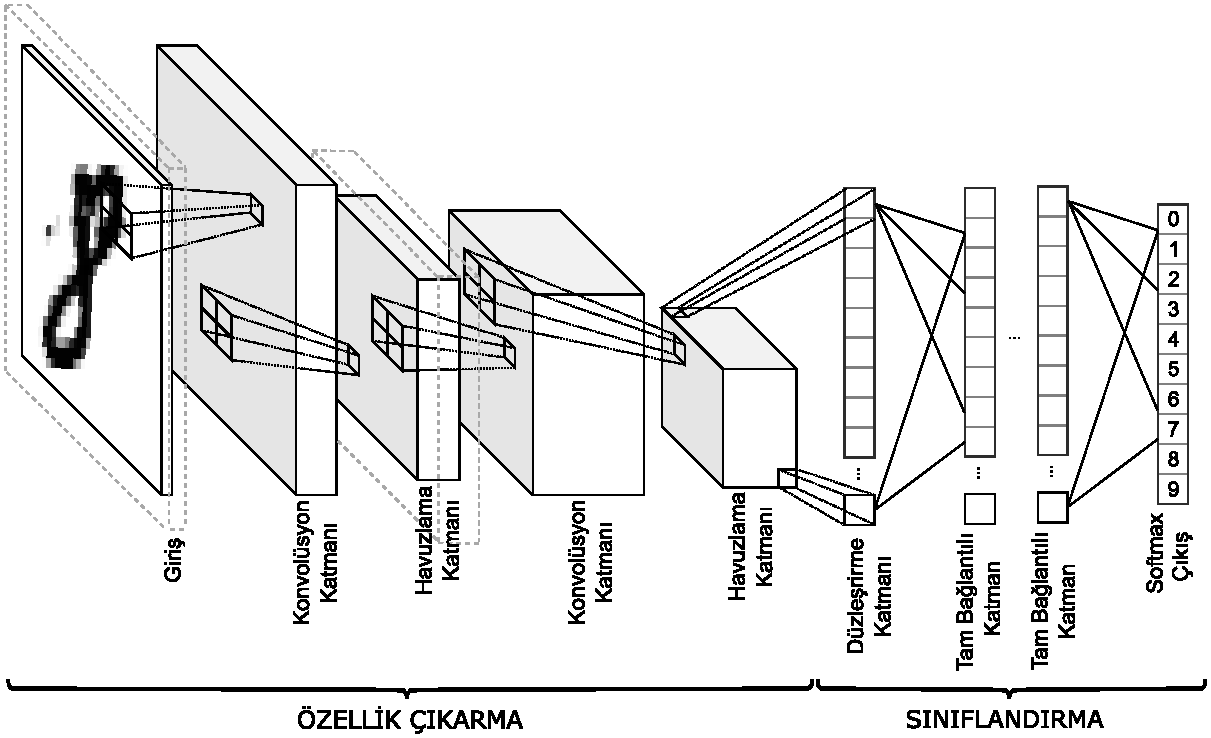
\includegraphics[scale=0.75]{Yapilan-Calismalar/Figures/cnn.pdf}
		}
	\end{center}
\end{figure}

\subsubsection{Konvolüsyonel Sinir Ağlarında Transfer Öğrenme}
Derin öğrenme sistemleri için gereken eğitim süresi ve veri miktarı geleneksel makine öğrenme sistemlerinden çok daha fazladır. Bilgisayarla görme ve doğal dil işleme gibi alanlarda geliştirilmiş ve test edilmiş, yüksek performansa sahip AlexNet \cite{krizhevsky2012imagenet}, VGG \cite{simonyan2014very}, GoogleNet \cite{szegedy2015going}, ResNet \cite{he2016deep}, MobileNet \cite{howard2017mobilenets}, EfficientNet \cite{tan2019efficientnet} gibi çeşitli derin öğrenme ağları mevcuttur. Bu modeller ImageNet \cite{deng2009imagenet} gibi oldukça fazla görüntü içeren veri tabanları ile yüksek güçlü GPU'lar kullanılarak eğitilmiş modellerdir.

\captionsetup[figure]{margin={0.2cm,0cm}}
\begin{figure}[h!]
	\begin{center}
		\vspace{0.4cm}
		\captionbox{AlexNet mimarisinden transfer öğrenme yapılarak el yazısı rakam sınıflandırma modeli.\label{fig:transfer_learning}}
		{
			\vspace{0.4cm}
			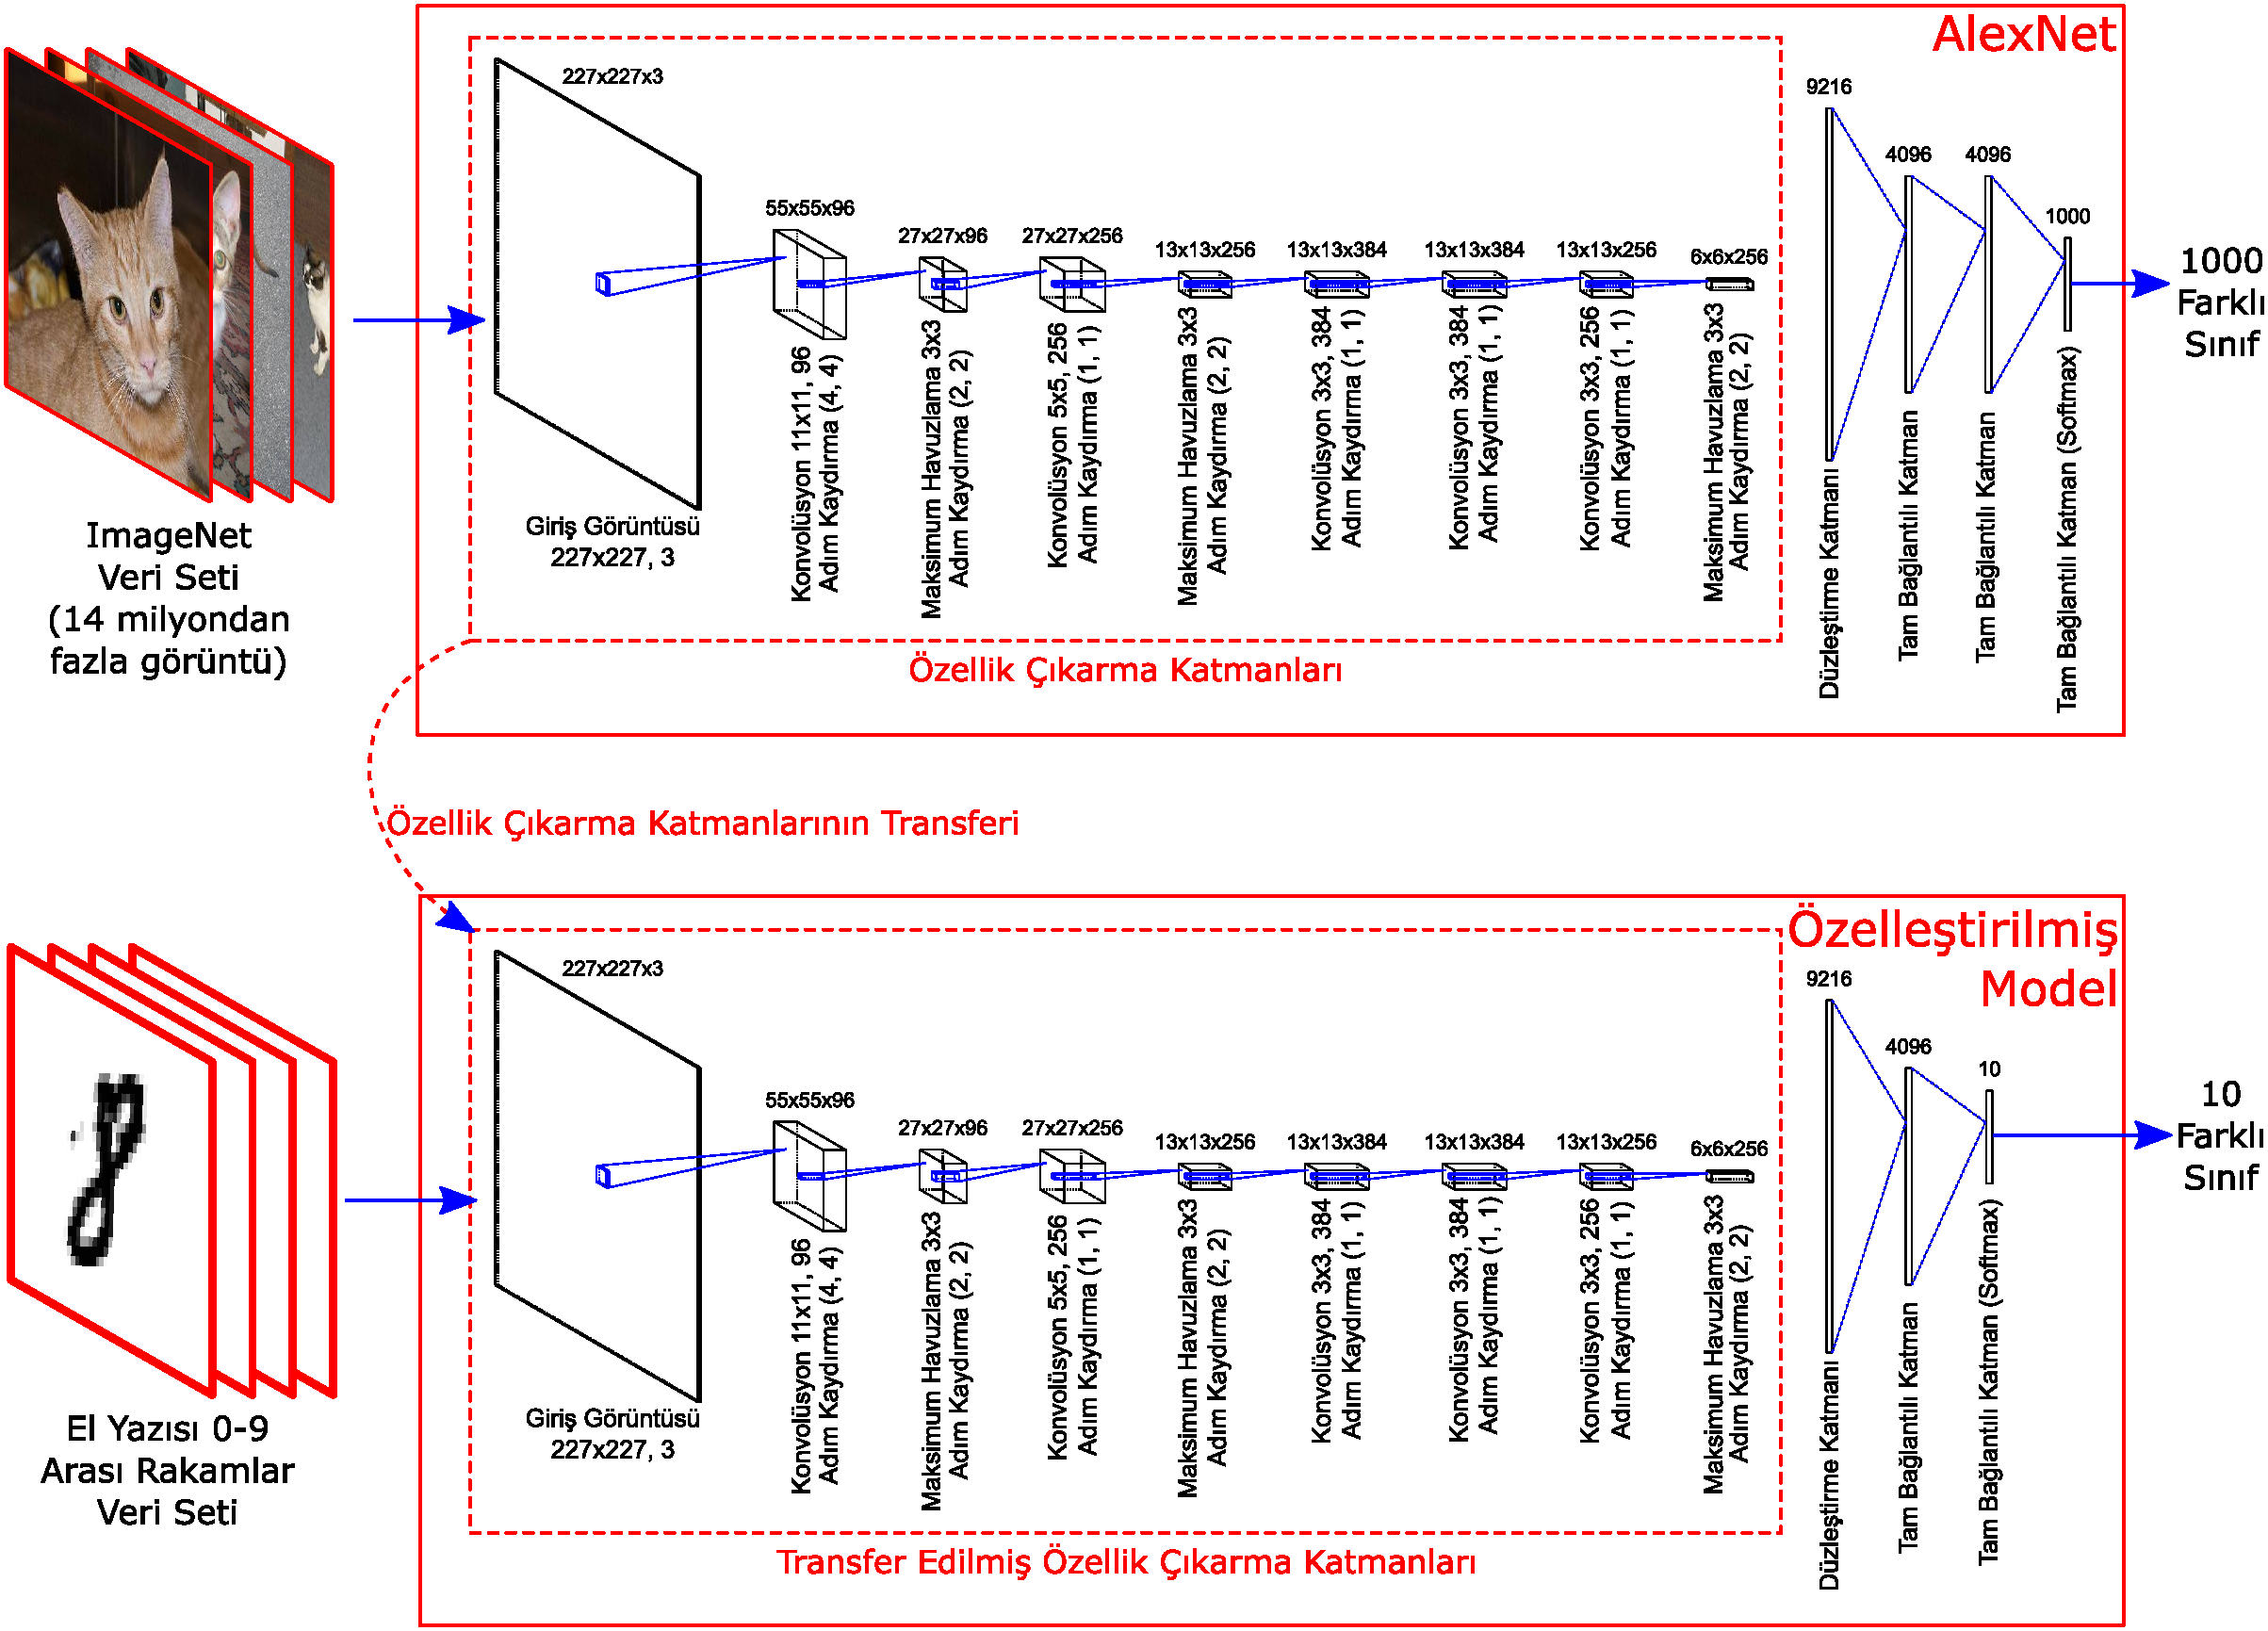
\includegraphics[scale=0.37]{Yapilan-Calismalar/Figures/transfer_learning.pdf}
		}
	\end{center}
\end{figure}

Model tabanlı transfer öğrenmedeki temel prensip daha önceden güçlü sistemler kullanılarak örnek sayısı bakımından zengin veri tabanları ile eğitilmiş yüksek performanslı modellerin özellik çıkarma katmanlarının alınarak başka sınıflandırıcı model ile birleştirilmesidir. Yeni birleştirilmiş modelde bambaşka bir veri seti kullanılarak sadece sınıflandırıcı katmanlarda eğitim gerçekleştirilmektedir. Böylece zamandan ve işlem gücünden tasarruf edilebilmektedir. Transfer edilen modelin yeni veri seti ile daha ileri seviye uyum sağlayabilmesi amaçlanmaktadır. Bu yüzden transfer edilen özellik çıkarma katmanlarının son birkaç katmanı eğitime tabi tutularak ince ayar (fine tunning) denilen eğitim gerçekleştirilmektedir. Derin özellik çıkarıcı katmanların ilk katmanları genellikle kenar doku bilgisi gibi daha genel özellik haritaları çıkarmak için özelleşirken daha derin ileri katmanları genellikle veri setine özgü özelliklerin öğrenilmesinde uzmanlaşmaktadır. Bu sebeple ince ayar ile birlikte veri setine özgü özelliklerin öğrenildiği özellik çıkarıcı katmanlar eğitime tabi tutulmakta ve veri setinin daha uygun özellik haritalarının elde edilmesi sağlanmaktadır.

Örneğin Şekil \ref{fig:transfer_learning}'de ImageNet veri tabanında eğitilmiş AlexNet mimarisi görülmektedir. Imagenet veri seti toplamda 14 milyondan fazla görüntüye sahip 1000 farklı sınıftan oluşmaktadır. ImageNet veri setinde eğitimi gerçekleştirilmiş AlexNet modelinin eğitilmiş özellik çıkarma katmanları Şekil \ref{fig:transfer_learning}'de gösterildiği gibi alınmıştır. 0 - 9 arasında el yazısı görüntülerinden oluşan bambaşka bir veri setine uygun sınıflandırma katmanları eklenmiştir. Bu modelde sadece sınıflandırma katmanlarının eğitimi gerçekleştirilebilmektedir. Bu eğitimde daha özel özellik haritaları üretebilmek için transfer öğrenme ile gelmiş özellik çıkarma katmanları istenen sayıda dahil edilerek eğitim gerçekleştirilebilmektedir. 

\subsection{Oto Kodlayıcılar}
Oto kodlayıcılar (Auto - encoders) girişinden verilen veriyi işleyerek çıkışından yine girişinden uygulanan veri ile aynı boyutlarda veri üreten derin ağlardır. Gürültü azaltma, veri sıkıştırma, veri bölütleme gibi çeşitli alanlarda kullanılmaktadır. Bu tez çalışmasında oto kodlayıcılar görüntü bölütleme amacıyla kullanılmıştır.

\captionsetup[figure]{margin={0.3cm,0.2cm}}
\begin{figure}[h!]
	\begin{center}
		\vspace{0.4cm}
		\captionbox{Oto-kodlayıcı kodlama ve kod çözme katmanları.\label{fig:autoencoder}}
		{
			\vspace{0.4cm}
			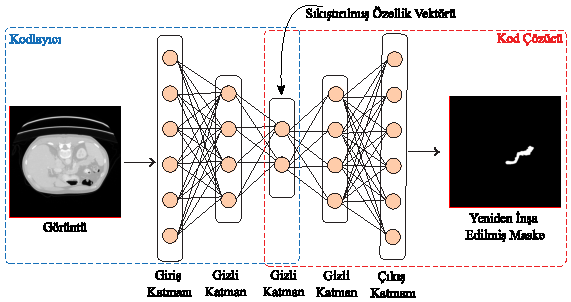
\includegraphics[scale=1.6]{Yapilan-Calismalar/Figures/autoencoder.pdf}
		}
	\end{center}
\end{figure}

Oto kodlayıcılar Şekil \ref{fig:autoencoder}'te gösterildiği gibi kodlama ve kod çözme katmanlarından oluşmaktadır. Oto kodlayıcılarla görüntü bölütleme gerçekleştirirken giriş görüntüsüne $x$, çıkışta inşa edilecek maske görüntüsü $r$, giriş $x$ görüntüsünün $f$ fonksiyonu ile kodlaması sonucu üretilecek sıkıştırılmış özellik vektörü $h$ ve sıkıştırılmış özellik vektöründen $r$ çıkış görüntüsünü elde etmek için gerekli kod çözücü fonksiyon $g$ olmak üzere, oto kodlayıcı kodlama denklemi Eşitlik \ref{eq:encode}, kod çözme denklemi ise Eşitlik \ref{eq:decode} ile temsil edilmektedir. Oto kodlayıcılarda öğrenilen bilgi $f(x)$ ve $g(h)$ fonksiyonları olmaktadır.
\begin{equation}
	\label{eq:encode}
	f(x)=h
\end{equation}
\vspace{-1.5cm}
\begin{equation}
	\label{eq:decode}
	g(h)=r
\end{equation}

\subsection{Derin Ağlarda Kullanılan Katmanlar}
Derin öğrenme çok fazla sayıda farklı türlerdeki katmanları birleştirerek çalıştırmayı gerektirmektedir. Örneğin ham veriden, veriye özgü özellik çıkarımı için konvolüsyon (evrişim) katmanları kullanılmaktadır. Ayrıca bu çıkarılan özelliklerin doğrusal olmamasını sağlayabilmek için doğrusal olmayan aktivasyon fonksiyonlarının kullanıldığı aktivasyon katmanları kullanılmaktadır. Konvolüsyon katmanlarından sonra ortaya çıkan yeni büyük ölçekli özellik haritalarının hesaplama maliyetinin azaltılması için mevcut verinin tekrar ölçeklenebilmesini sağlayan havuzlama katmanları kullanılmaktadır. Ayrıca sınıflandırma problemlerinde özellik çıkarma katmanlarından elde edilen özellik haritalarından sınıf tahmini yapabilen sınıflandırma katmanları bulunmaktadır. Derin öğrenme modelleri bunların dışında birçok farklı eğitilebilir ya da eğitilemeyen katmanlardan oluşabilmektedirler. Katmanlar birbirleri ile bir zincirin halkaları gibi bağlı olduğu için modelin eğitiminde genellikle gradyan öğrenme teknikleri tercih edilmektedir. Eğitilebilir bütün katmanlarda bir sonraki katmandan gelen türev bilgisi kullanılarak eğitim optimizasyonu gerçekleştirilmektedir. Eğitilemeyen havuzlama, düzleştirme gibi katmanlar eğitim aşamasında sadece türevin bir önceki katmana taşınmasını sağlamaktadırlar.

%\iffalse
%\begin{table}[h!]
%	\begin{tabular}{lll}
%		Konvolüsyon Katmanı      & Conv1D, Conv2D, Conv3D                            &  \\
%		Ters Konvolüsyon Katmanı & Conv1DTranspose, Conv2DTranspose, Conv3DTranspose &  \\
%		Sık Örnekleme Katmanı    & UpSampling1D, UpSampling2D, UpSampling3D          &  \\
%		Aktivasyon Katmanları    & Sigmoid,Tanh, ReLU,PReLU,ELU                      &  \\
%		Normalizasyon Katmanları & Normalization, BatchNormalization          &  \\
%		Birleştirme Katmanları   & Add, Concatenate          &  \\
%		Havuzlama Katmanları   & Add, Concatenate          &  \\
%	\end{tabular}
%\end{table} 
%\fi

\subsubsection{Tam Bağlantılı Katmanlar}
Tam Bağlantılı (Fully Connected - FC) katmanlar aslında derin öğrenme mimarilerinin sınıflandırıcı katmanlarını temsil etmektedir. Yoğun (Dense) katman olarak da adlandırılmaktadırlar. Temelde derin öğrenme çalışmaları için İleri Beslemeli Sinir Ağları (Feed Forward Neural Network - FNN) mimarilerinden biri olan Çok Katmanlı Algılayıcılar (Multi Layer Perceptron - MLP) mimarisi tercih edilmekte ve derin öğrenmeyi anlayabilmek için MLP mimarisinin matematiksel modelini anlamak gerekmektedir.

\captionsetup[figure]{margin={0.4cm,-3cm}}
\begin{figure}[h!]
	\begin{center}
		\vspace{0.4cm}
		\captionbox{MLP mimarisinin temelini oluşturan algılayıcı blok diyagramı\label{fig:perceptron}}
		{
			\vspace{0.4cm}
			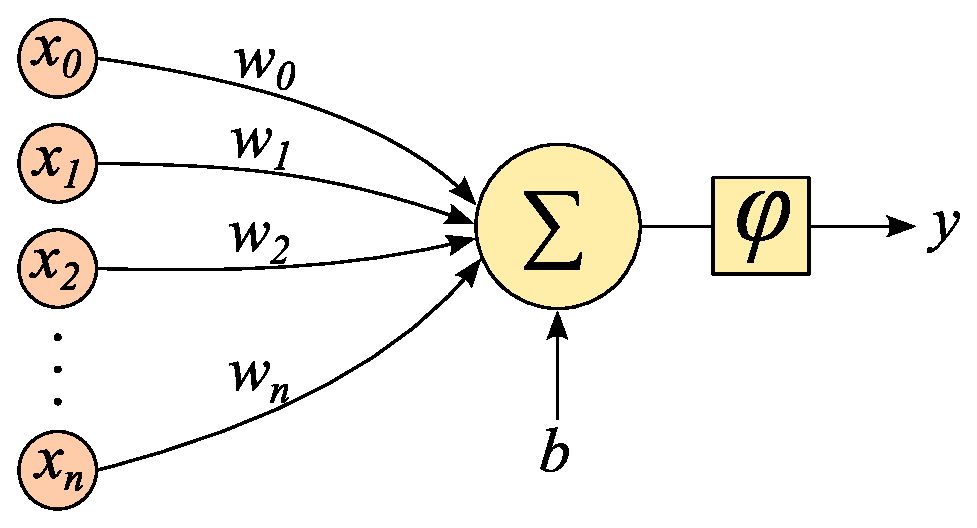
\includegraphics[scale=0.55]{Yapilan-Calismalar/Figures/perceptron.pdf}
		}
	\end{center}
\end{figure}

İlk Algılayıcı (Perceptron) matematiksel modeli 1958 yılında ortaya atılmıştır \cite{rosenblatt1957perceptron}. Başlangıçta hiperdüzlem üzerindeki doğrusal problemin çözümüne yönelik geliştirilen algılayıcılar, doğrusal olmayan aktivasyon fonksiyonlarını kullanan MLP mimarisine geçilerek hiper düzlem üzerinde doğrusal dağılmamış verilerin sınıflandırılması içinde kullanılabilir hale getirilmiştir. Algılayıcılar insan sinir hücresinin basit bir modelli gibi çalışmaktadır. Algılayıcı modeli girişinden $x_{0}, x_{1},..., x_{n}$ şeklinde  $n$ adet elemana sahip bir vektör almaktadır. Giriş vektörünün her bir elemanı kendisine karşılık gelen $w_{0}, w_{1},..., w_{n}$ ağırlıkları ile çarpılarak ana düğümde toplanmaktadır. Bu yaklaşımda girişten gelen $x$ değerlerinin hepsinin sıfır olması durumunda $w$ ağırlık değerlerinin anlamsızlaşabileceği için genel toplama bir yanlılık (bias - $b$) değeri eklenmektedir. Genel toplam doğrusal olmayan ve öğrenme aşamasında kullanım kolaylığı sağlaması amacıyla türevi hesaplanabilir bir aktivasyondan ($\varphi$ ) geçirilmekte ve Şekil \ref{fig:perceptron}'te gösterildiği gibi bir $y$ çıkışı elde edilmektedir. 

Algılayıcının girişinden uygulanan $x$ değerleri ile $y$ çıkışının hesaplanması Eşitlik \ref{eq:perceptron}'te verildiği gibi gerçekleştirilmektedir.
\begin{equation}
	\label{eq:perceptron}
	y = \varphi(\sum_{i}w_{i}x_{i} + b)
\end{equation}

\captionsetup[figure]{margin={0.4cm,-3cm}}
\begin{figure}[h!]
	\begin{center}
		\vspace{0.2cm}
		\captionbox{Tam bağlantılı katmanın blok diyagramı\label{fig:ithlayer}}
		{
			\vspace{0.2cm}
			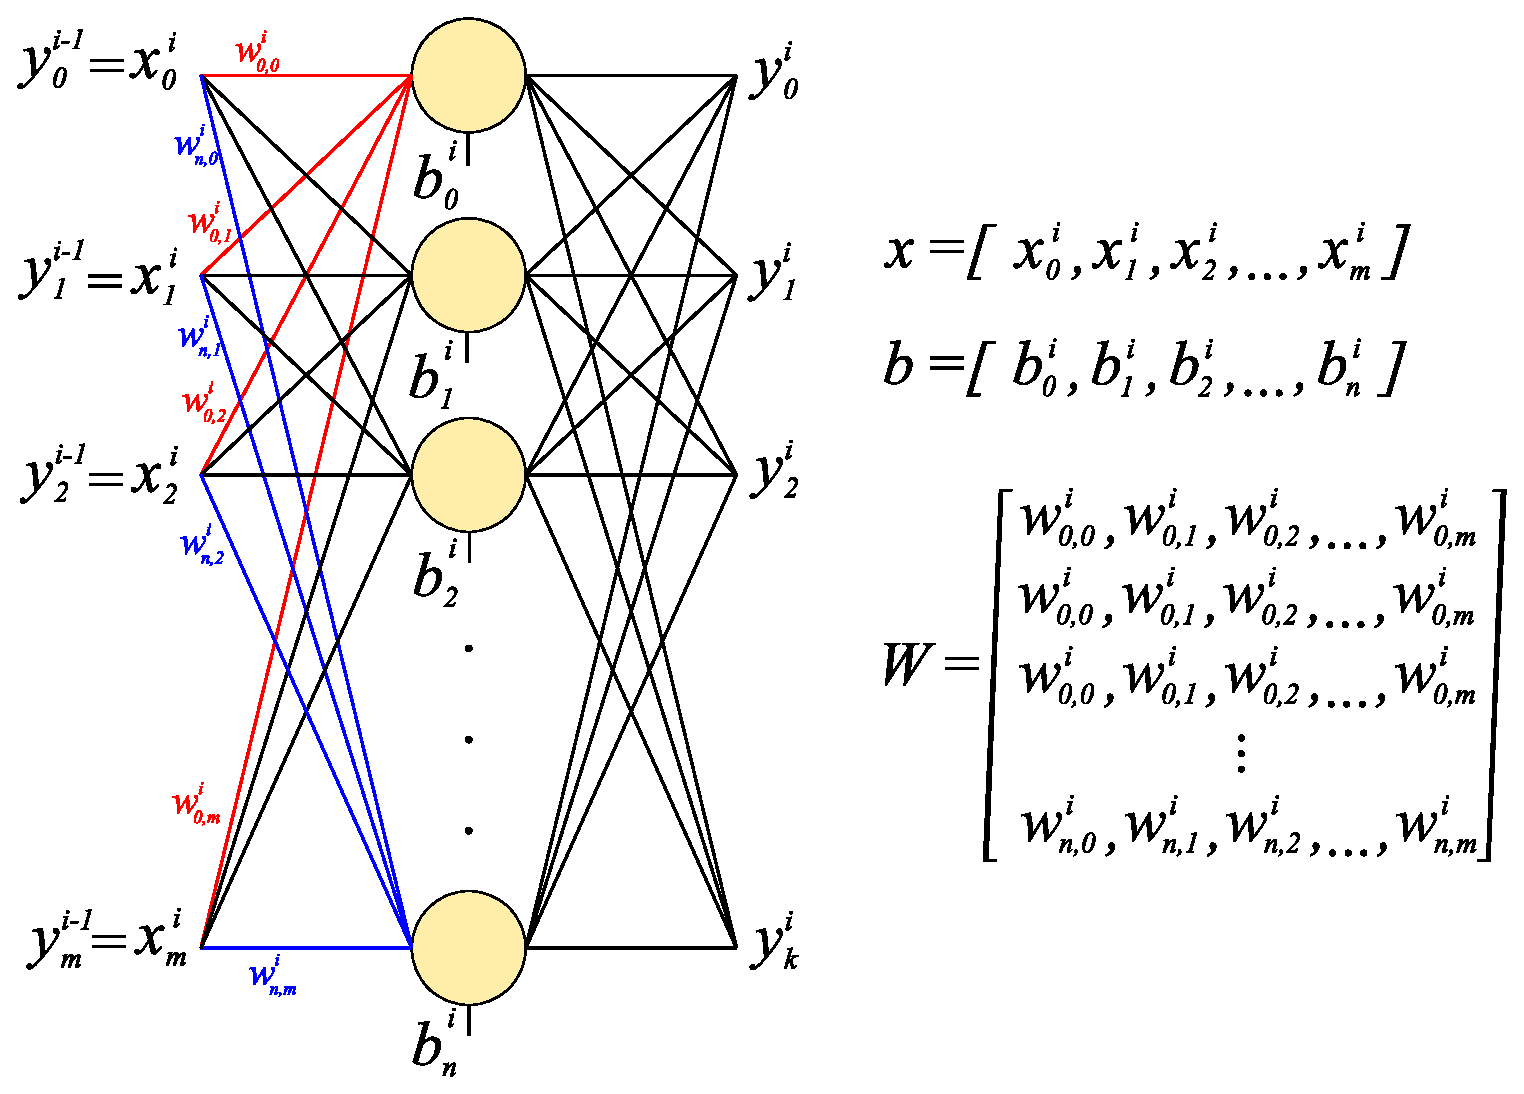
\includegraphics[scale=0.55]{Yapilan-Calismalar/Figures/ithlayer.pdf}
		}
	\end{center}
\end{figure}

Çok katmanlı ve her bir katmanında farklı sayılarda algılayıcılardan oluşan bir mimari düşünüldüğünde herbir algılayıcı çıkışının ayrı ayrı hesaplanması gerekmektedir. Bu tip yapılarda $m$ bir önceki $i-1$ inci katmandan gelen giriş değerlerinin adetini göstermek üzere $i$ inci katmandaki $x$ giriş ifadelerini $\overset{\rightarrow}{x} = \left[ x_{0}^{i}, x_{1}^{i}, x_{2}^{i},..., x_{m}^{i} \right]$ şeklinde bir vektör olarak düşünürsek. Yine ilgili $i$ inci katmandaki $n$ adet algılayıcının yanlılık $b$ değerlerini de $\overset{\rightarrow}{b} = \left[ b_{0}^{i}, b_{1}^{i}, b_{2}^{i},..., b_{n}^{i} \right]$ şeklinde bir vektör olarak düşünmek gerekmektedir. Bu doğrultuda $i-1$ inci katmandan gelen her bir girişin tam bağlantılı olarak $i$ inci katmandaki algılayıcılara giden ağırlıkları Şekil \ref{fig:ithlayer}'te gösterildiği gibi $W$ şeklinde bir matris ile temsil etmek gerekmektedir.  

Çok algılayıcılı katman mimarisi için gerekli vektör, matris dönüşümleri gerçekleştirildikten sonra tam bağlantılı katmanın ileri yönde hesaplaması Eşitlik \ref{eq:fclayer}'teki gibi gerçekleştirilerek $\overset{\rightarrow}{y}$ çıkış vektörü hesaplanabilmektedir. 
\begin{equation}
	\label{eq:fclayer}
	y = \varphi(Wx + b)
\end{equation} 

Eşitlik \ref{eq:fclayer}'te $\varphi$ aktivasyon fonksiyonunu temsil etmektedir. Varsayılan aktivasyon fonksiyonu $f(x) = x$ şeklindeki Doğrusal Aktivasyon fonksiyonudur. Bu katmanda aktivasyon fonksiyonu belirtilebileceği gibi tamamen farklı bir katmanmış gibi bu katmanın ardından aktivasyon katmanı eklenerek de kurulacak çok katmanlı mimarinin doğrusal olmayan çıkışlar üretmesi sağlanabilmektedir.

Tam bağlantılı katman ardından yine bir katman eklenebileceği gibi direk çıkış katmanı olarak da kullanılabilmektedir. Tam bağlantılı katman çıkış katmanı olarak kullanıldığında bu katmanda kullanılan aktivasyon fonksiyonu modelin eğitiminde kullanılacak optimizasyon tekniğini de belirleyen etken olarak karşımıza çıkmaktadır. Aynı zamanda verinin eğitim etiketlerinin hangi aralıkta olması gerektiğini de belirleyen faktör aktivasyon fonksiyonunun karakteristiğidir. 

\captionsetup[figure]{margin={0.3cm,-2.5cm}}
\begin{figure}[h!]
	\begin{center}
		\vspace{0.4cm}
		\captionbox{Tam bağlantılı katmanda bir sonraki katmandan gelen hata bilgisine göre zincir kuralı kullanılarak kısmi türevlerin hesaplanması\label{fig:perceptronDerivative}}
		{
			\vspace{0.4cm}
			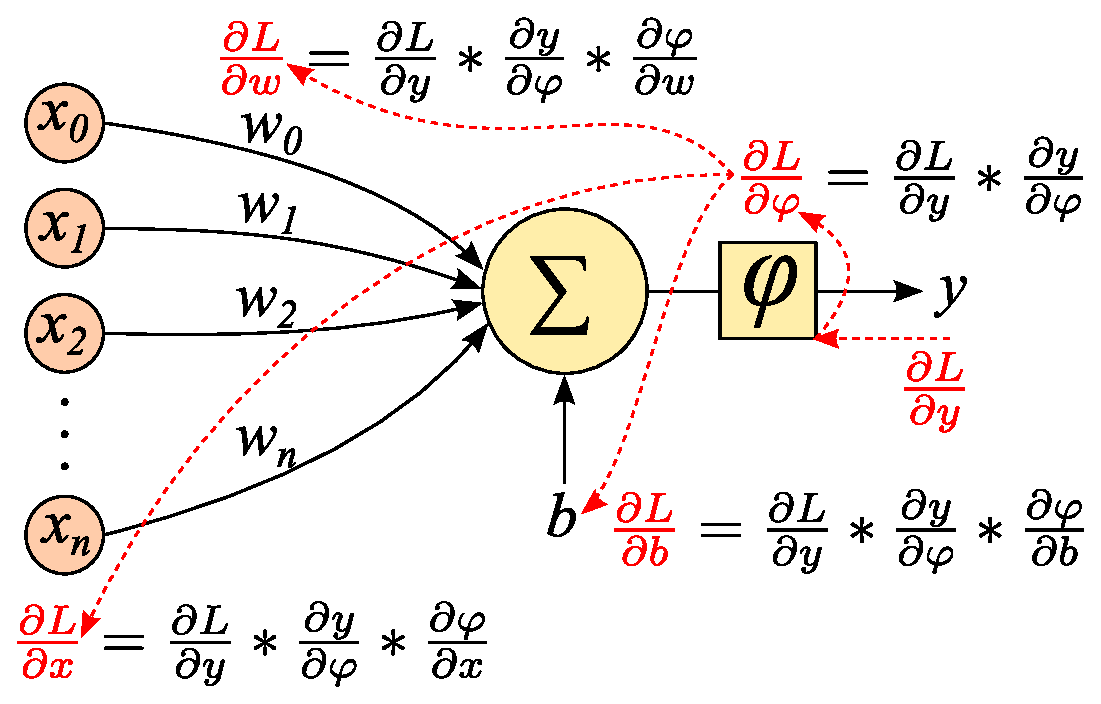
\includegraphics[scale=0.55]{Yapilan-Calismalar/Figures/perceptronDerivative.pdf}
		}
	\end{center}
\end{figure}

Tam bağlantılı katmanlarda eğitim, ağırlık ($W$) ve yanlılık ($b$) parametrelerinde gerçekleştirilmektedir. Çok katmanlı mimarilerin tüm katmanlarında olduğu gibi tam bağlantılı katmanlarda da eğitim ağın genel kayıp fonksiyonunun gradyanı kullanılarak gerçekleştirilmektedir. Bu sebeple güncellenecek tüm eğitilebilir parametrelerde bir sonraki katmandan gelen hata bilgisine $\frac{\partial L}{\partial  y}$ göre zincir kuralı kullanılarak kısmi türevlerin hesaplanması gerekmektedir. Şekil \ref{fig:perceptronDerivative}'da bir sinir hücresinin bir sonraki katmandan gelen $\frac{\partial L}{\partial  y}$ hata bilgisine göre ağırlık ($W$) ve  yanlılık ($b$) bilgilerini eğitim için güncelleştirilmesinde kullanılacak kısmi türev hesabı gösterilmektedir. $x$ giriş ifadelerindeki kısmi türev hesabı ilgili katmanın ara katman olması durumunda hatanın ilk katmanlara iletiminde kullanılması olmaktadır. Eğer kısmi türevi hesaplanan katman giriş katmanı ise $x$ değerleri için hesaplanan değerler kullanılmamaktadır.

Sinir hücresi çıkışı $y$'nin bir sonraki katmandan gelen hataya göre kısmi türevi $\frac{\partial L}{\partial  y}$ olmak üzere $W$ ve $b$ değerlerini eğitebilmek için gerekli kısmi türev bilgisi sırasıyla Eşitlik \ref{eq:wderivative}, \ref{eq:bderivative} ve \ref{eq:xderivative}'de verilmektedir. Ayrıca $x$ girişleri için ilgili katmandan bir önceki katmana iletilecek hatanın kısmi türevi de Eşitlik \ref{eq:xderivative} kullanılarak hesaplanabilmektedir.
\begin{equation}
	\label{eq:wderivative}
	\frac{\partial L}{\partial  w} = \frac{\partial L}{\partial  y}* \frac{\partial y}{\partial  \varphi} * \frac{\partial  \varphi}{\partial  w}
\end{equation}
\vspace{-1cm} 
\begin{equation}
	\label{eq:bderivative}
	\frac{\partial L}{\partial  b} = \frac{\partial L}{\partial  y}* \frac{\partial y}{\partial  \varphi} * \frac{\partial  \varphi}{\partial  b}
\end{equation} 
\vspace{-1cm}
\begin{equation}
	\label{eq:xderivative}
	\frac{\partial L}{\partial  x} = \frac{\partial L}{\partial  y}* \frac{\partial y}{\partial  \varphi} * \frac{\partial  \varphi}{\partial  x}
\end{equation} 

\subsubsection{Konvolüsyon Katmanları}

Konvolüsyonel Sinir Ağları (CNN) en önemli derin öğrenme ağlarından biridir. Bu sinir ağı modelinde konvolüsyon katmanları, girdi olarak verilen sinyal, görüntü ya da 3B volümetrik veriden otomatik özellik çıkarma işlemini gerçekleştirmektedir. Konvolüsyon katmanları el yazısı ile yazılmış zip kodlarını tanımaya yönelik geliştirilen bir çalışmada ilk kez kullanılmıştır \cite{lecun1989backpropagation}.

Konvolüsyon katmanları CNN mimarisinin yapı taşlarıdır. Özellik çıkarımı yapılacak verinin boyutlarına göre yapılandırılabilmektedir. Bu sayede ham veri 1B bir sinyal ise 1B konvolüsyon filtreleri kullanılarak 1B uzayda özellik çıkarma işlemi yapılabilmektedir. Aynı şekilde veri 2B bir görüntü ise 2B konvolüsyon filtreleri kullanılarak 2B uzayda özellik çıkarma işlemi gerçekleştirilebilmektedir. Verinin 3B volümetrik bir veri olması durumunda ise 3B konvolüsyon filtreleri kullanılarak 3B özellik çıkarma işlemi gerçekleştirilebilmektedir. Konvolüsyonel katmanlarda öğrenilen bilgi ham veriye uygulanan konvolüsyon filtrelerinin değerleri olmaktadır. Bu tez çalışmasında tek kanallı laboratuvar görüntüleri kullanıldığı için konvolüsyon işlemi tek kanallı gri seviye görüntüler üzerinde gerçekleştirilmektedir.

$G$ konvolüsyonu hesaplanacak görüntü, $F$ konvolüsyon filtresi, $i$ değeri görüntünün $x$ yatay eksendeki indeksi, $j$ değeri görüntünün $y$ dikey eksendeki indeksi olmak üzere $O$ konvolüsyon işlemi sonucu ortaya çıkacak özellik haritası Eşitlik \ref{eq:konvolusyon}'deki gibi hesaplanmaktadır.
\begin{equation}
	\label{eq:konvolusyon}
	O(i, j)=(F * G)(i, j)=\sum_{m} \sum_{n} G(i-m, j-n) F(m, n)
\end{equation}

Konvolüsyon işlemi 1B, 2B ve 3B filtreler kullanılarak mevcut işlenecek veriye göre özelleştirilebilmektedir. Konvolüsyon katmanı ile istenen sayıda ve ebatlarda konvolüsyon filtreleri seçilebilmektedir. Ayrıca konvolüsyon filtrelerinin görüntüye uygulanma sırasında Adım Kaydırma (Stride) miktarı da özelleştirilebilmektedir. Konvolüsyon işlemi sonucunda ortaya çıkan özellik haritalarının ebatları herhangi bir Dolgulama (Padding) işlemi gerçekleştirilmediğinde konvolüsyon filtresinin ebatlarına bağlı olarak küçülmektedir. Şekil \ref{fig:conv2d}'de örnek bir 2B görüntü için filtre sayısı 1 ve dolgulama miktarı 0 seçildiğinde konvolüsyon işleminin ilk üç adımı sırasıyla yeşil, mavi ve kırmızı renklerde gösterilmektedir. Adım kaydırma miktarının konvolüsyon işlemi üzerindeki etkisi de yine bu görselde vurgulanmaktadır. Şekil \ref{fig:conv2d}'de görüldüğü gibi adım kaydırma miktarının değişimi elde edilen özellik haritasının ebatlarını direkt belirleyen faktörlerden biridir. 

\captionsetup[figure]{margin={0.3cm,0cm}}
\begin{figure}[h!]
	\begin{center}
		\vspace{0.4cm}
		\captionbox{Filtre sayısı 1 ve dolgulama miktarı 0 seçildiğinde 2B konvolüsyon ve adım kaydırma işlemleri. \label{fig:conv2d}}
		{
			\vspace{0.4cm}
			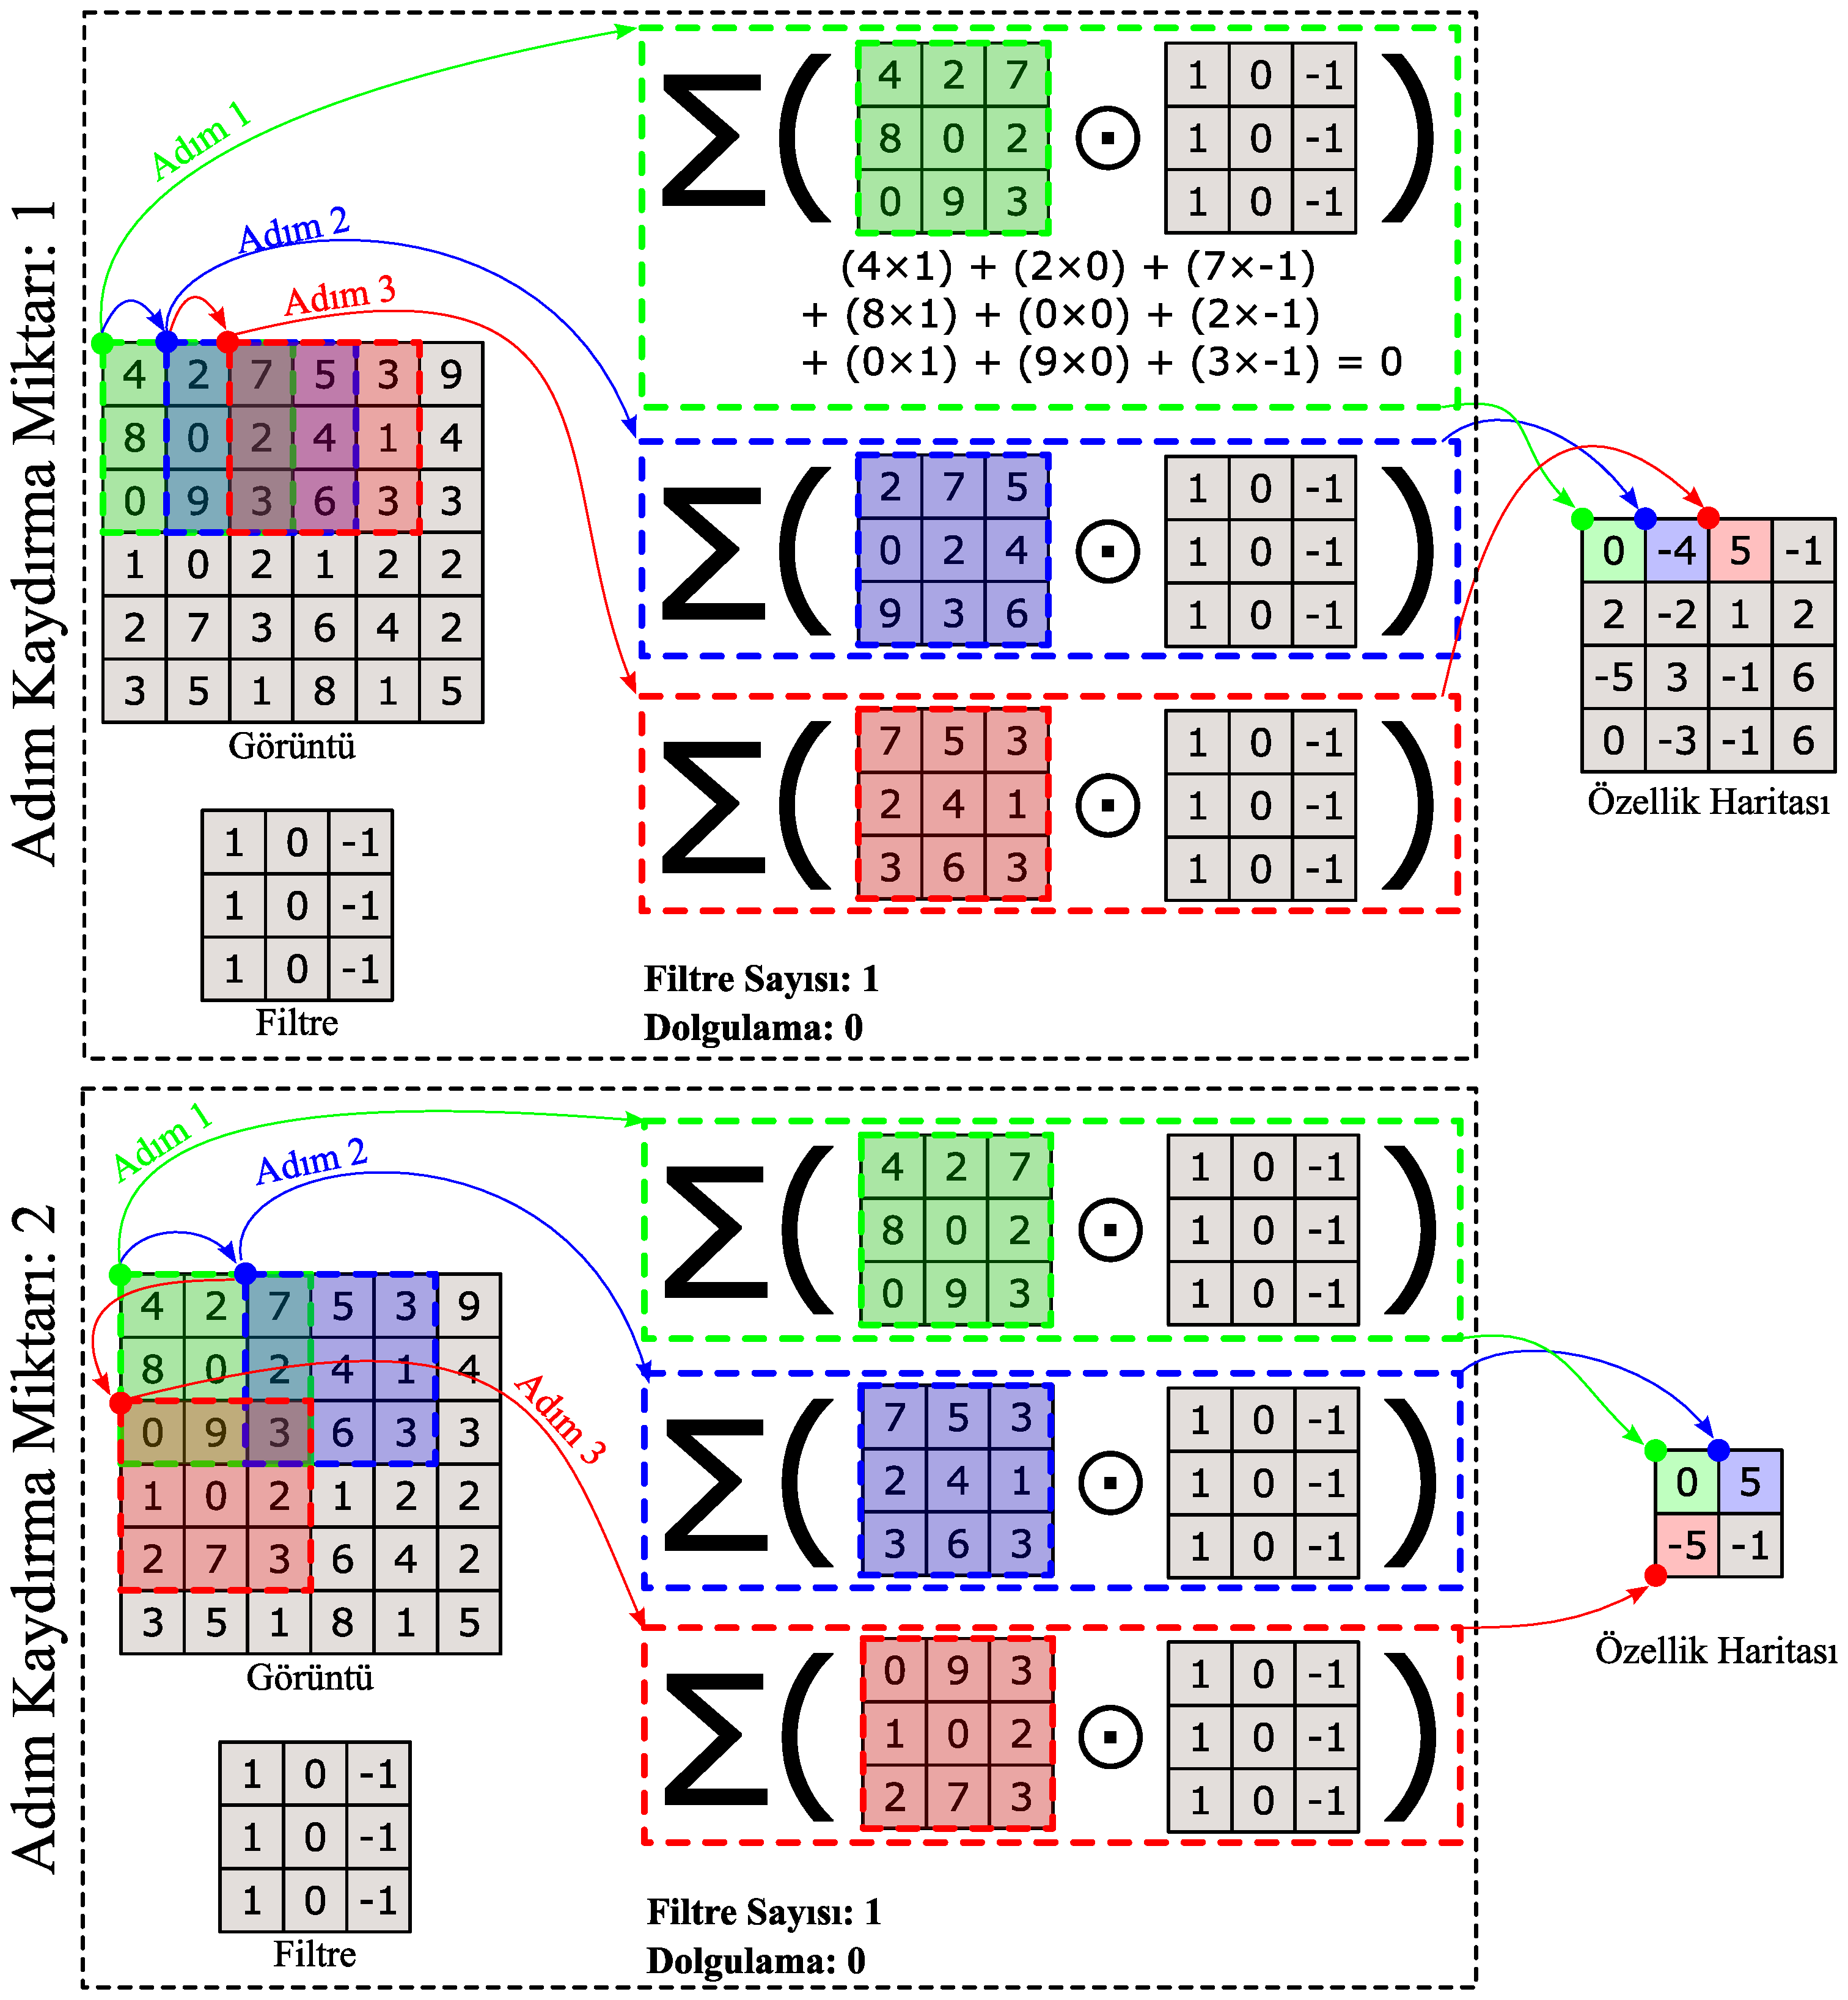
\includegraphics[scale=0.3]{Yapilan-Calismalar/Figures/conv2D2.pdf}
		}
	\end{center}
\end{figure}

Konvolüsyon filtrelerinin sayısı Şekil \ref{fig:conv_sizes}'de gösterildiği gibi konvolüsyon işlemi sonucu ortaya çıkacak özellik haritalarının sayısı ile eşit olmaktadır. Bunun sebebi giriş görüntüsüne konvolüsyon filtrelerinin birbirinden bağımsız uygulanması ve her konvolüsyon filtresinin yeni bir özellik haritası çıkarmasıdır. Ayrıca herhangi bir dolgulama işlemi gerçekleştirilmediğinde konvolüsyon filtrelerinin ebatlarına bağlı olarak hesaplanan özellik haritalarının ebatları giriş görüntüsünden farklı olmaktadır. 

\captionsetup[figure]{margin={0.3cm,-0.2cm}}
\begin{figure}[h!]
	\begin{center}
		\vspace{0.4cm}
		\captionbox{Konvolüsyon işlemi sonrası filtre sayısına bağlı olarak ortaya çıkan özellik haritaları. \label{fig:conv_sizes}}
		{
			\vspace{0.4cm}
			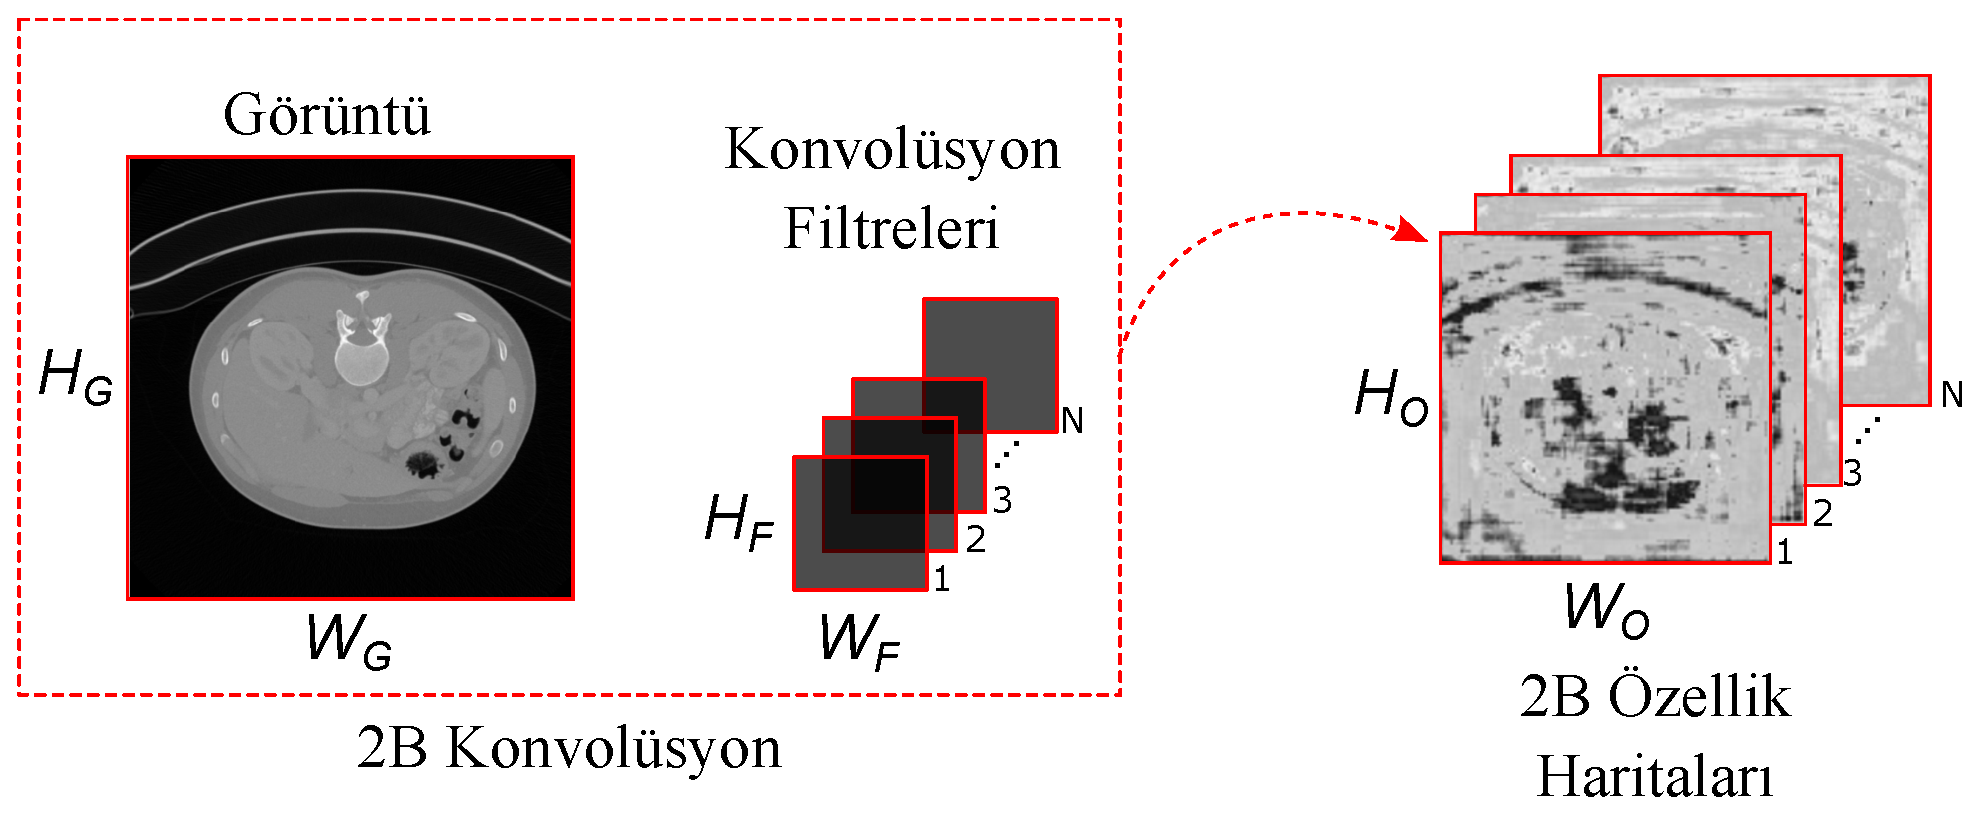
\includegraphics[scale=0.44]{Yapilan-Calismalar/Figures/conv_sizes.pdf}
		}
	\end{center}
\end{figure}

Konvolüsyon işleminde giriş görüntüsünün genişliği $W_{G}$, yüksekliği $H_{G}$, konvolüsyon filtrelerinin genişliği $W_{F}$, yüksekliği $H_{F}$, konvolüsyon işlemi sırasında konvolüsyon filtresinin adım kaydırma miktarı $s$ ve dolgulama miktarı $p$, hesaplanacak özellik haritalarının genişliği $W_{O}$, yüksekliği $H_{O}$ olmak üzere, bu tez çalışmasında kullanılan veri setlerinde giriş verisinin genişlik ve yükseklik değerlerinin eşit uzunlukta olması ve eşit uzunluklu filtreler tercih edildiğinden dolayı giriş verisi ebatları $W_{G}=H_{G}=G$, konvolüsyon filtresi ebatları $W_{F}=H_{F}=F$ olarak kabul edilirse çıkış özellik haritasının ebatları $W_{O}=H_{O}=O$ Eşitlik \ref{eq:featuremapsize}'daki gibi hesaplanabilmektedir.
\begin{equation}
	\label{eq:featuremapsize}
	O=\left\lfloor \frac{G-F+2p}{s}+1 \right\rfloor
\end{equation}

Bu çalışmada 2B konvolüsyon işlemleri gerçekleştirildiği gibi 3B konvolüsyon işlemleri de gerçekleştirilmektedir. 3B konvolüsyon işleminde giriş görüntüleri 3B volümetrik verilerden oluşmaktadır. Bu volümetrik verilere konvolüsyon işlemi 3B konvolüsyon filtreleri ile 2B konvolüsyon işleminde olduğu gibi adım kaydırma ve dolgulama işlemleri ile uygulanabilmektedir. 3B volümetrik görüntülerde 3B konvolüsyon filtrelerinin gezdirilmesine yönelik görsel Şekil \ref{fig:conv3d}'da gösterilmektedir.

\captionsetup[figure]{margin={0.5cm,-2.2cm}}
\begin{figure}[h!]
	\begin{center}
		\vspace{0.4cm}
		\captionbox{3B volümetrik görüntülerde 3B konvolüsyon filtrelerinin gezdirilmesi.\label{fig:conv3d}}
		{
			\vspace{0.4cm}
			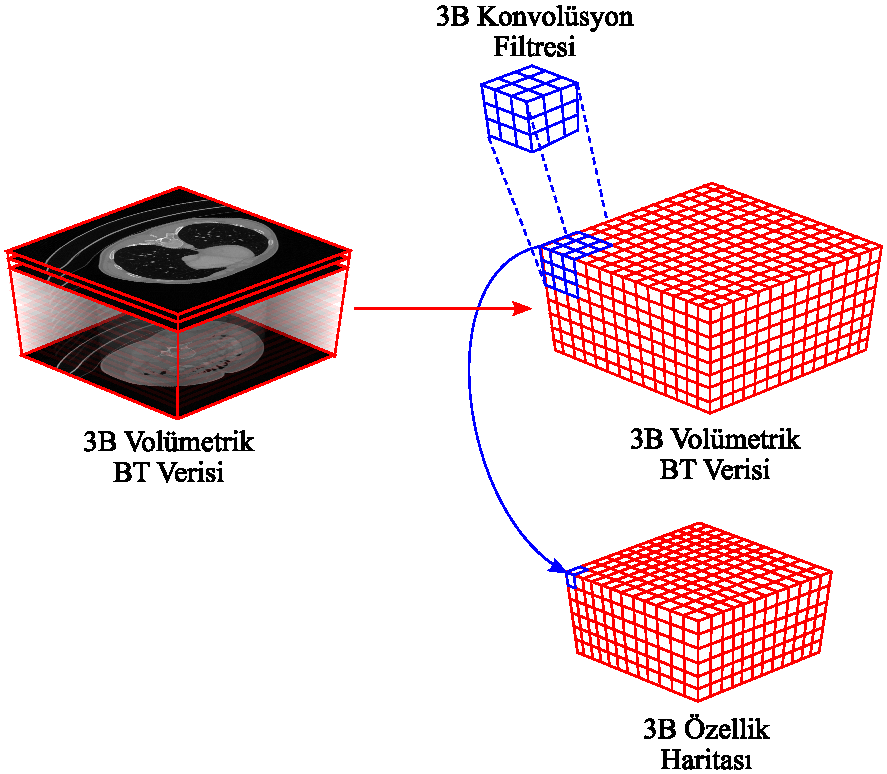
\includegraphics[scale=0.7]{Yapilan-Calismalar/Figures/conv3D.pdf}
		}
	\end{center}
\end{figure}

Konvolüsyon işleminde hesaplanan özellik haritalarının ebatlarının giriş görüntü ebatları ile aynı olmasının istenildiği durumlarda dolgulama işlemi gerçekleştirilmektedir. 2B görüntüde dolgulama işlemi gerçekleştirerek konvolüsyon özellik haritası hesaplama işlemi Şekil \ref{fig:conv2Dpadding}'da gösterilmektedir. Görüldüğü gibi giriş görüntüsü $0$ değerli bir çerçeve içerisine alınarak konvolüsyon işlemi gerçekleştirilmektedir. Özellikle konvolüsyon filtrelerinin ebatları büyüdüğünde görüntüden hesaplanan özellik haritalarının ebatları oldukça düşmektedir. Dolgulama işlemi ile bu problem büyük ölçüde ortadan kaldırılabilmektedir.

\captionsetup[figure]{margin={0.2cm,-3cm}}
\begin{figure}[h!]
	\begin{center}
		\vspace{0.4cm}
		\captionbox{2B konvolüsyon işleminde dolgulama işlemi.\label{fig:conv2Dpadding}}
		{
			\vspace{0.4cm}
			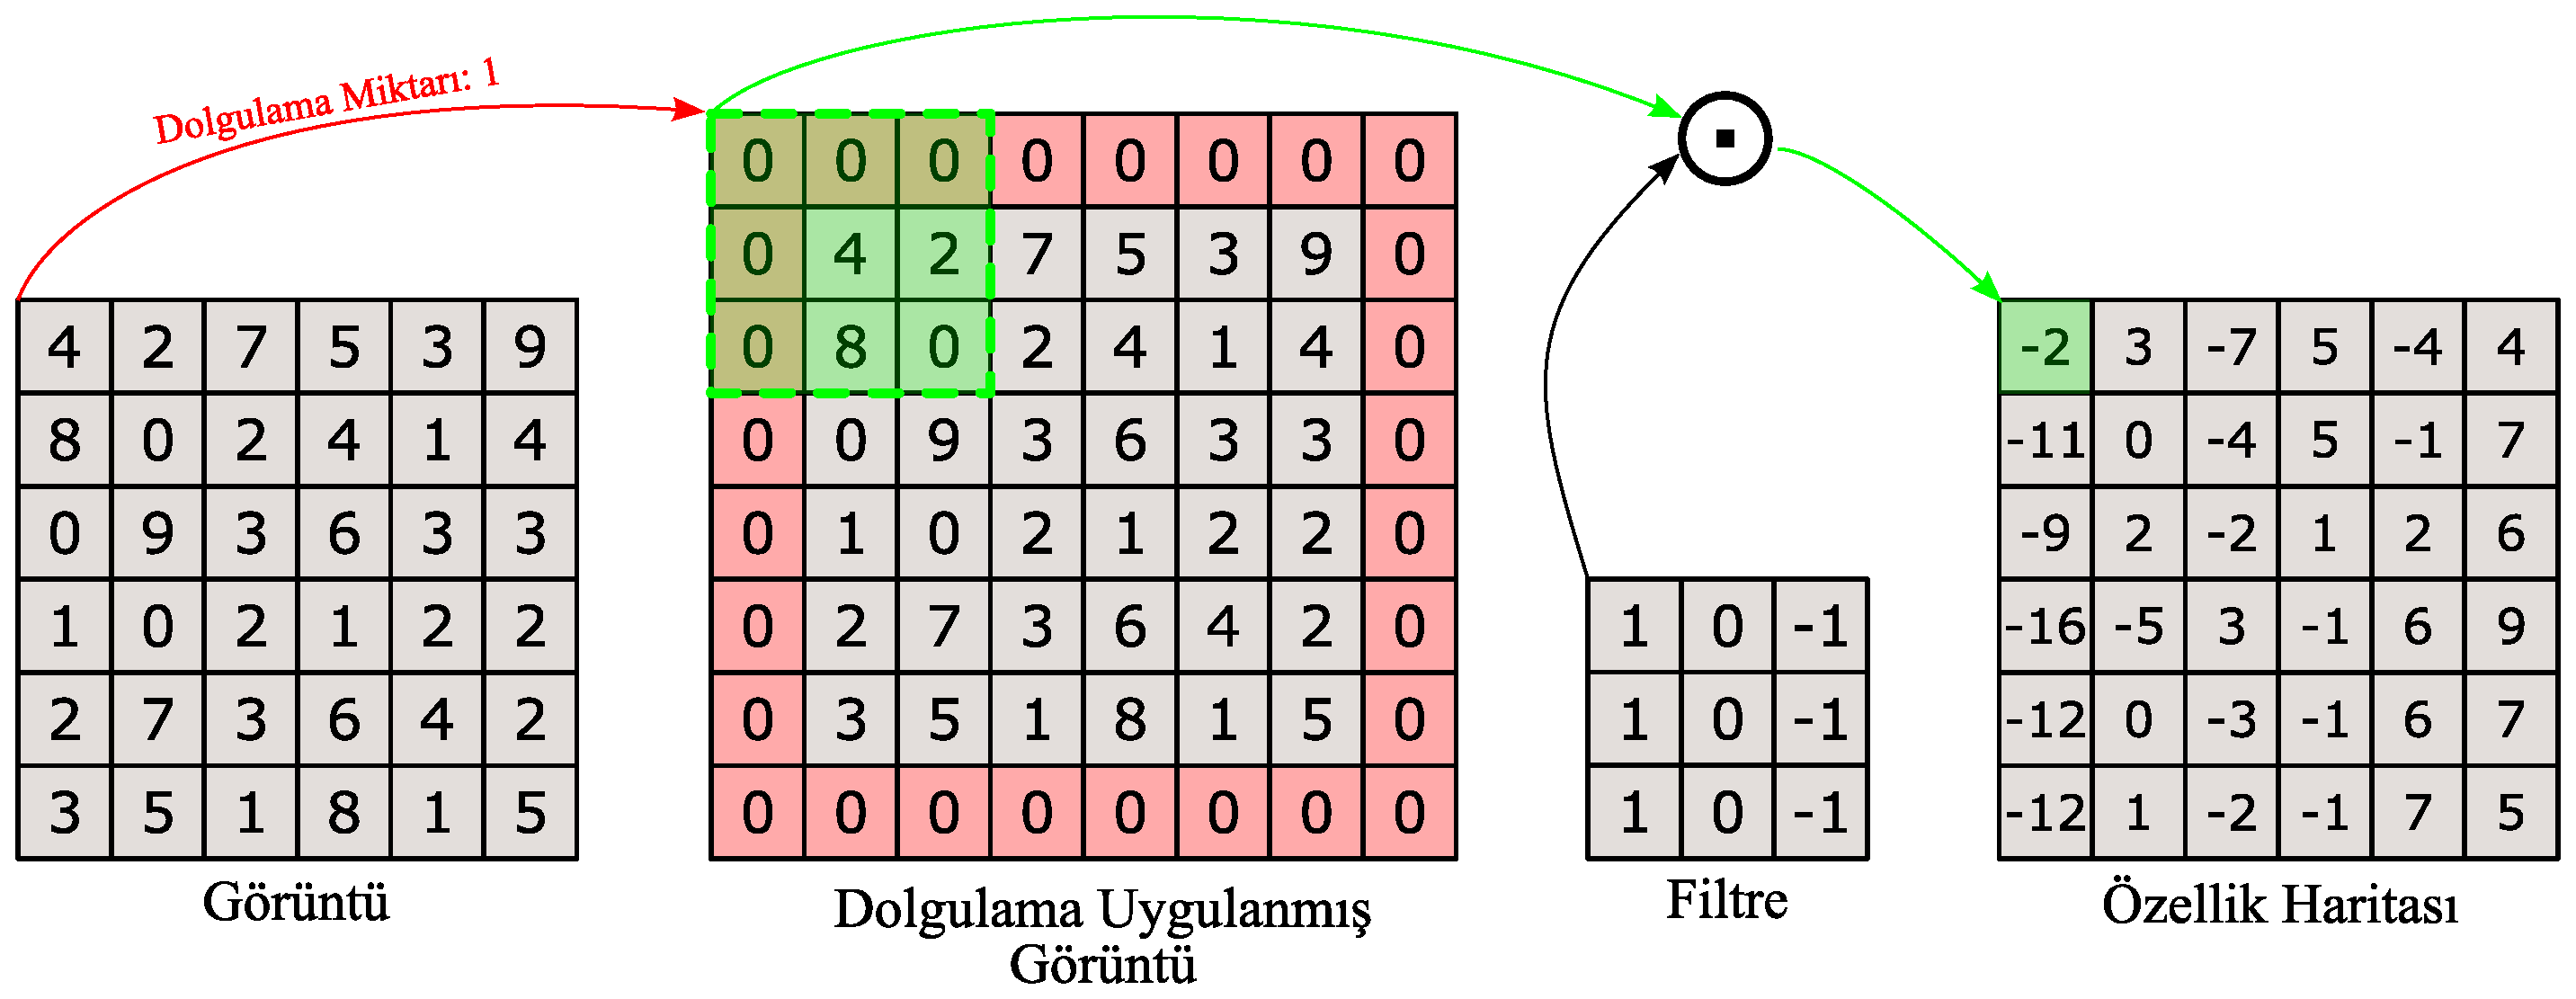
\includegraphics[scale=0.32]{Yapilan-Calismalar/Figures/conv2Dpadding.pdf}
		}
	\end{center}
\end{figure}

Konvolüsyon işleminde dolgulama miktarı $p$, filtre ebatları $F$ olmak üzere dolgulama miktarı Eşitlik \ref{eq:padding}'daki gibi hesaplanabilmektedir.
\begin{equation}
	\label{eq:padding}
	p=\frac{F-1}{2}
\end{equation}

Konvolüsyon katmanlarında eğitim $F$ filtre parametreleri üzerinde gerçekleştirilmektedir. Tüm diğer katmanlarda olduğu gibi konvolüsyon katmanında da eğitim gerçekleştirebilmek için modelin genel hatasının zincir kuralına göre gradyanının hesaplanılması gerekmektedir. Konvolüsyon katmanına uygulanan giriş verisi $G$ ve konvolüsyon katmanının çıkışı $O$ olmak üzere bir sonraki katmandan gelen hatanın kısmi türevi $\frac{\partial L}{\partial  O}$ ile $F$ filtre parametrelerini güncellemek için hesaplanılması gereken $\frac{\partial L}{\partial  F}$ kısmi türevinin zincir kuralına göre geri yayılımı Şekil \ref{fig:convDerivative}'de gösterilmektedir. Bu kısmi türev Eşitlik \ref{eq:convFderivative} kullanılarak hesaplanmaktadır.
\begin{equation}
	\label{eq:convFderivative}
	\frac{\partial L}{\partial  F} = \frac{\partial L}{\partial  O}* \frac{\partial O}{\partial  F}
\end{equation}

\captionsetup[figure]{margin={0.2cm,-3cm}}
\begin{figure}[h!]
	\begin{center}
		\vspace{0.4cm}
		\captionbox{Hatanın geri yayılımı ile konvolüsyon katmanının kısmi türevleri.\label{fig:convDerivative}}
		{
			\vspace{0.4cm}
			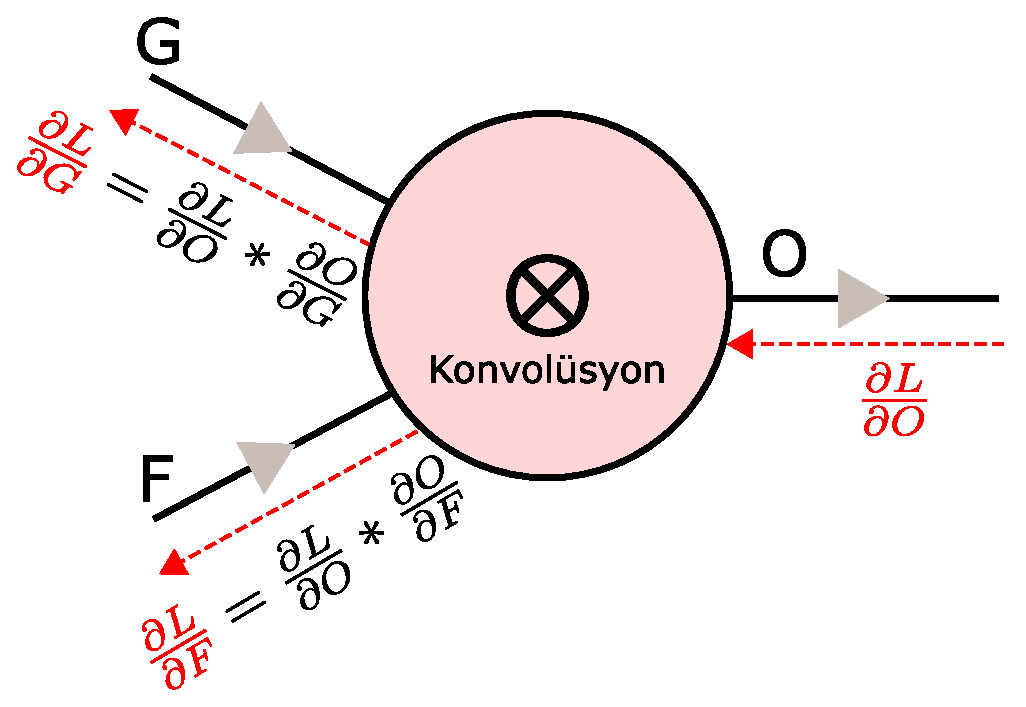
\includegraphics[scale=0.6]{Yapilan-Calismalar/Figures/convDerivative.pdf}
		}
	\end{center}
\end{figure}

İlgili konvolüsyon katmanından önceki katmanlara hatanın yayılımı $G$ görüntü girişi yönündeki $\frac{\partial L}{\partial  G}$ kısmi türevi Eşitlik \ref{eq:convGderivative} kullanılarak hesaplanmaktadır. Önceki katmanlardaki zincir kuralına benzer şekilde uygulanarak eğitilebilir parametrelerin güncellenmesi sağlanmaktadır.
\begin{equation}
	\label{eq:convGderivative}
	\frac{\partial L}{\partial  G} = \frac{\partial L}{\partial  O}* \frac{\partial O}{\partial  G}
\end{equation}


\subsubsection{Ters Konvolüsyon Katmanları}

Konvolüsyon katmanları dolgulama yapılmadığı taktirde girişlerinden uygulanan verilerden özellik çıkarırlarken giriş verisi boyutları küçültülmektedir. Özellikle oto-kodlayıcılarda bu boyut küçültme işlemi kodlama işlemi olarak adlandırılmaktadır. Oto-kodlayıcıların girişinden uygulanan verilerde gürültü azaltma, görüntü bölütleme v.b. işlemler gerçekleştirebilmektedir. Oto-kodlayıcılarda hiyerarşik olarak giriş verisi boyutları küçültülerek kodlama işlemi yapılmakta ve girişten uygulanan verinin kompleks özellik haritaları elde edilmektedir. Bu özellik haritalarından ters yönde hiyerarşik olarak boyut artırarak giriş verisiyle eşit boyutlarda görüntüler elde edebilmek için ters konvolüsyon katmanları kullanılabilmektedir. Dolayısıyla ters konvolüsyon katmanları genellikle konvolüsyon katmanlarından sonra hesaplanan özellik haritalarının eski boyutlarına getirilmesinde kullanılmaktadır.

\captionsetup[figure]{margin={0.5cm,-0.5cm}}
\begin{figure}[h!]
	\begin{center}
		\vspace{0.4cm}
		\captionbox{Adım kaydırma miktarı 1, Filtre sayısı 1 ve dolgulama miktarı 0 seçildiğinde 2B Ters Konvolüsyon işlemi.\label{fig:conv2Dtranspose1}}
		{
			\vspace{0.4cm}
			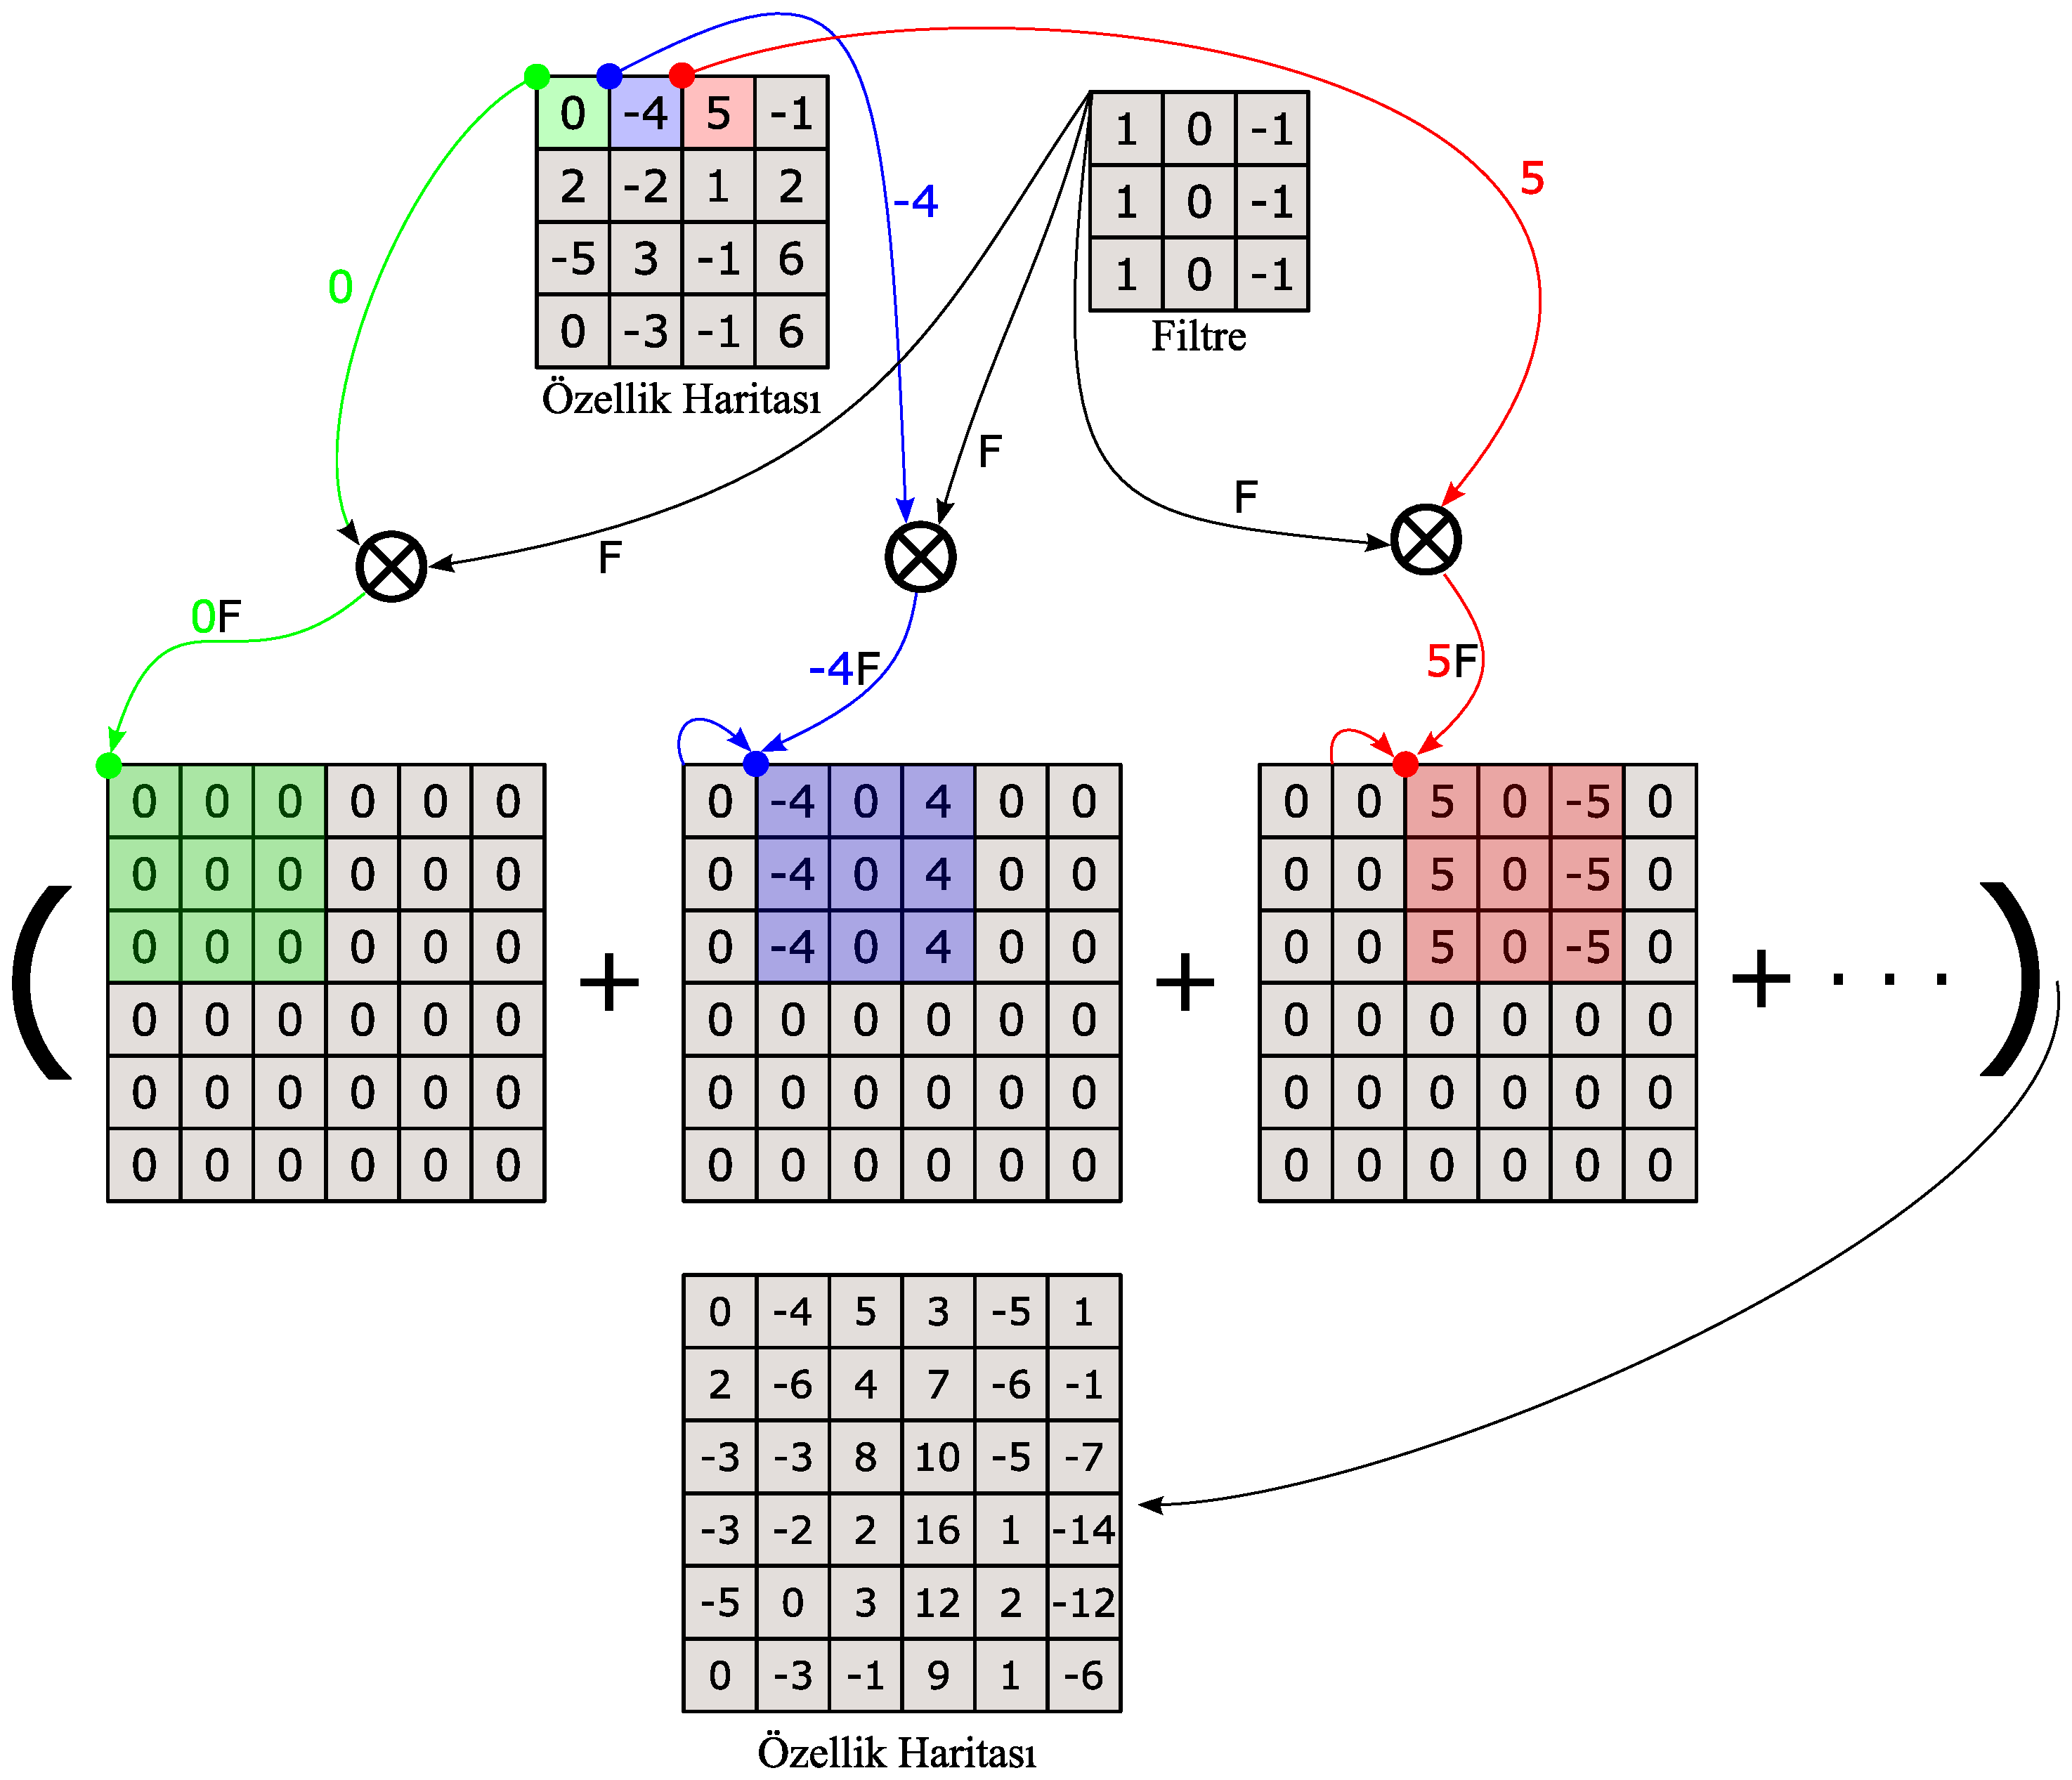
\includegraphics[scale=0.28]{Yapilan-Calismalar/Figures/conv2Dtranspose1.pdf}
		}
	\end{center}
\end{figure}

Ters konvolüsyon işleminde öncelikle ters konvolüsyon sonrası ortaya çıkacak özellik haritasının boyutlarını belirlemek gerekmektedir. Konvolüsyon işlemi sonucunda girişten uygulanan verinin boyutları küçültülürken, ters konvolüsyon işleminde girişten uygulanan verinin boyutları büyütülmektedir. Ters konvülüsyon işleminde giriş özellik haritasının ebatları $G$, filtre ebatları $F$, dolgulama miktarı $p$, adım kaydırma miktarı $s$ olmak üzere çıkış $O$ özellik haritasının ebatları Eşitlik \ref{eq:convtrans} kullanılarak hesaplanabilmektedir. Bu eşitlikte $\alpha$ katsayısı ters konvolüsyon işleminde görüntü ebatlarının istenen ebatlara ölçeklenebilmesi için kullanıcı tanımlı hiper parametredir. $\alpha$ parametresine adım kaydırma miktarı $s=1$ değerinden farklı olduğunda ihtiyaç duyulmaktadır.
\begin{equation}
	\label{eq:convtrans}
	O=s(G-1)+\alpha+k-2p \text{ , } \alpha\in\left\{ 0,...,s-1 \right\}
\end{equation}

\captionsetup[figure]{margin={0.4cm,-0.8cm}}
\begin{figure}[h!]
	\begin{center}
		\vspace{0.4cm}
		\captionbox{Adım kaydırma miktarı 2, Filtre sayısı 1 ve dolgulama miktarı 0 seçildiğinde 2B Ters Konvolüsyon işlemi.\label{fig:conv2Dtranspose2}}
		{
			\vspace{0.4cm}
			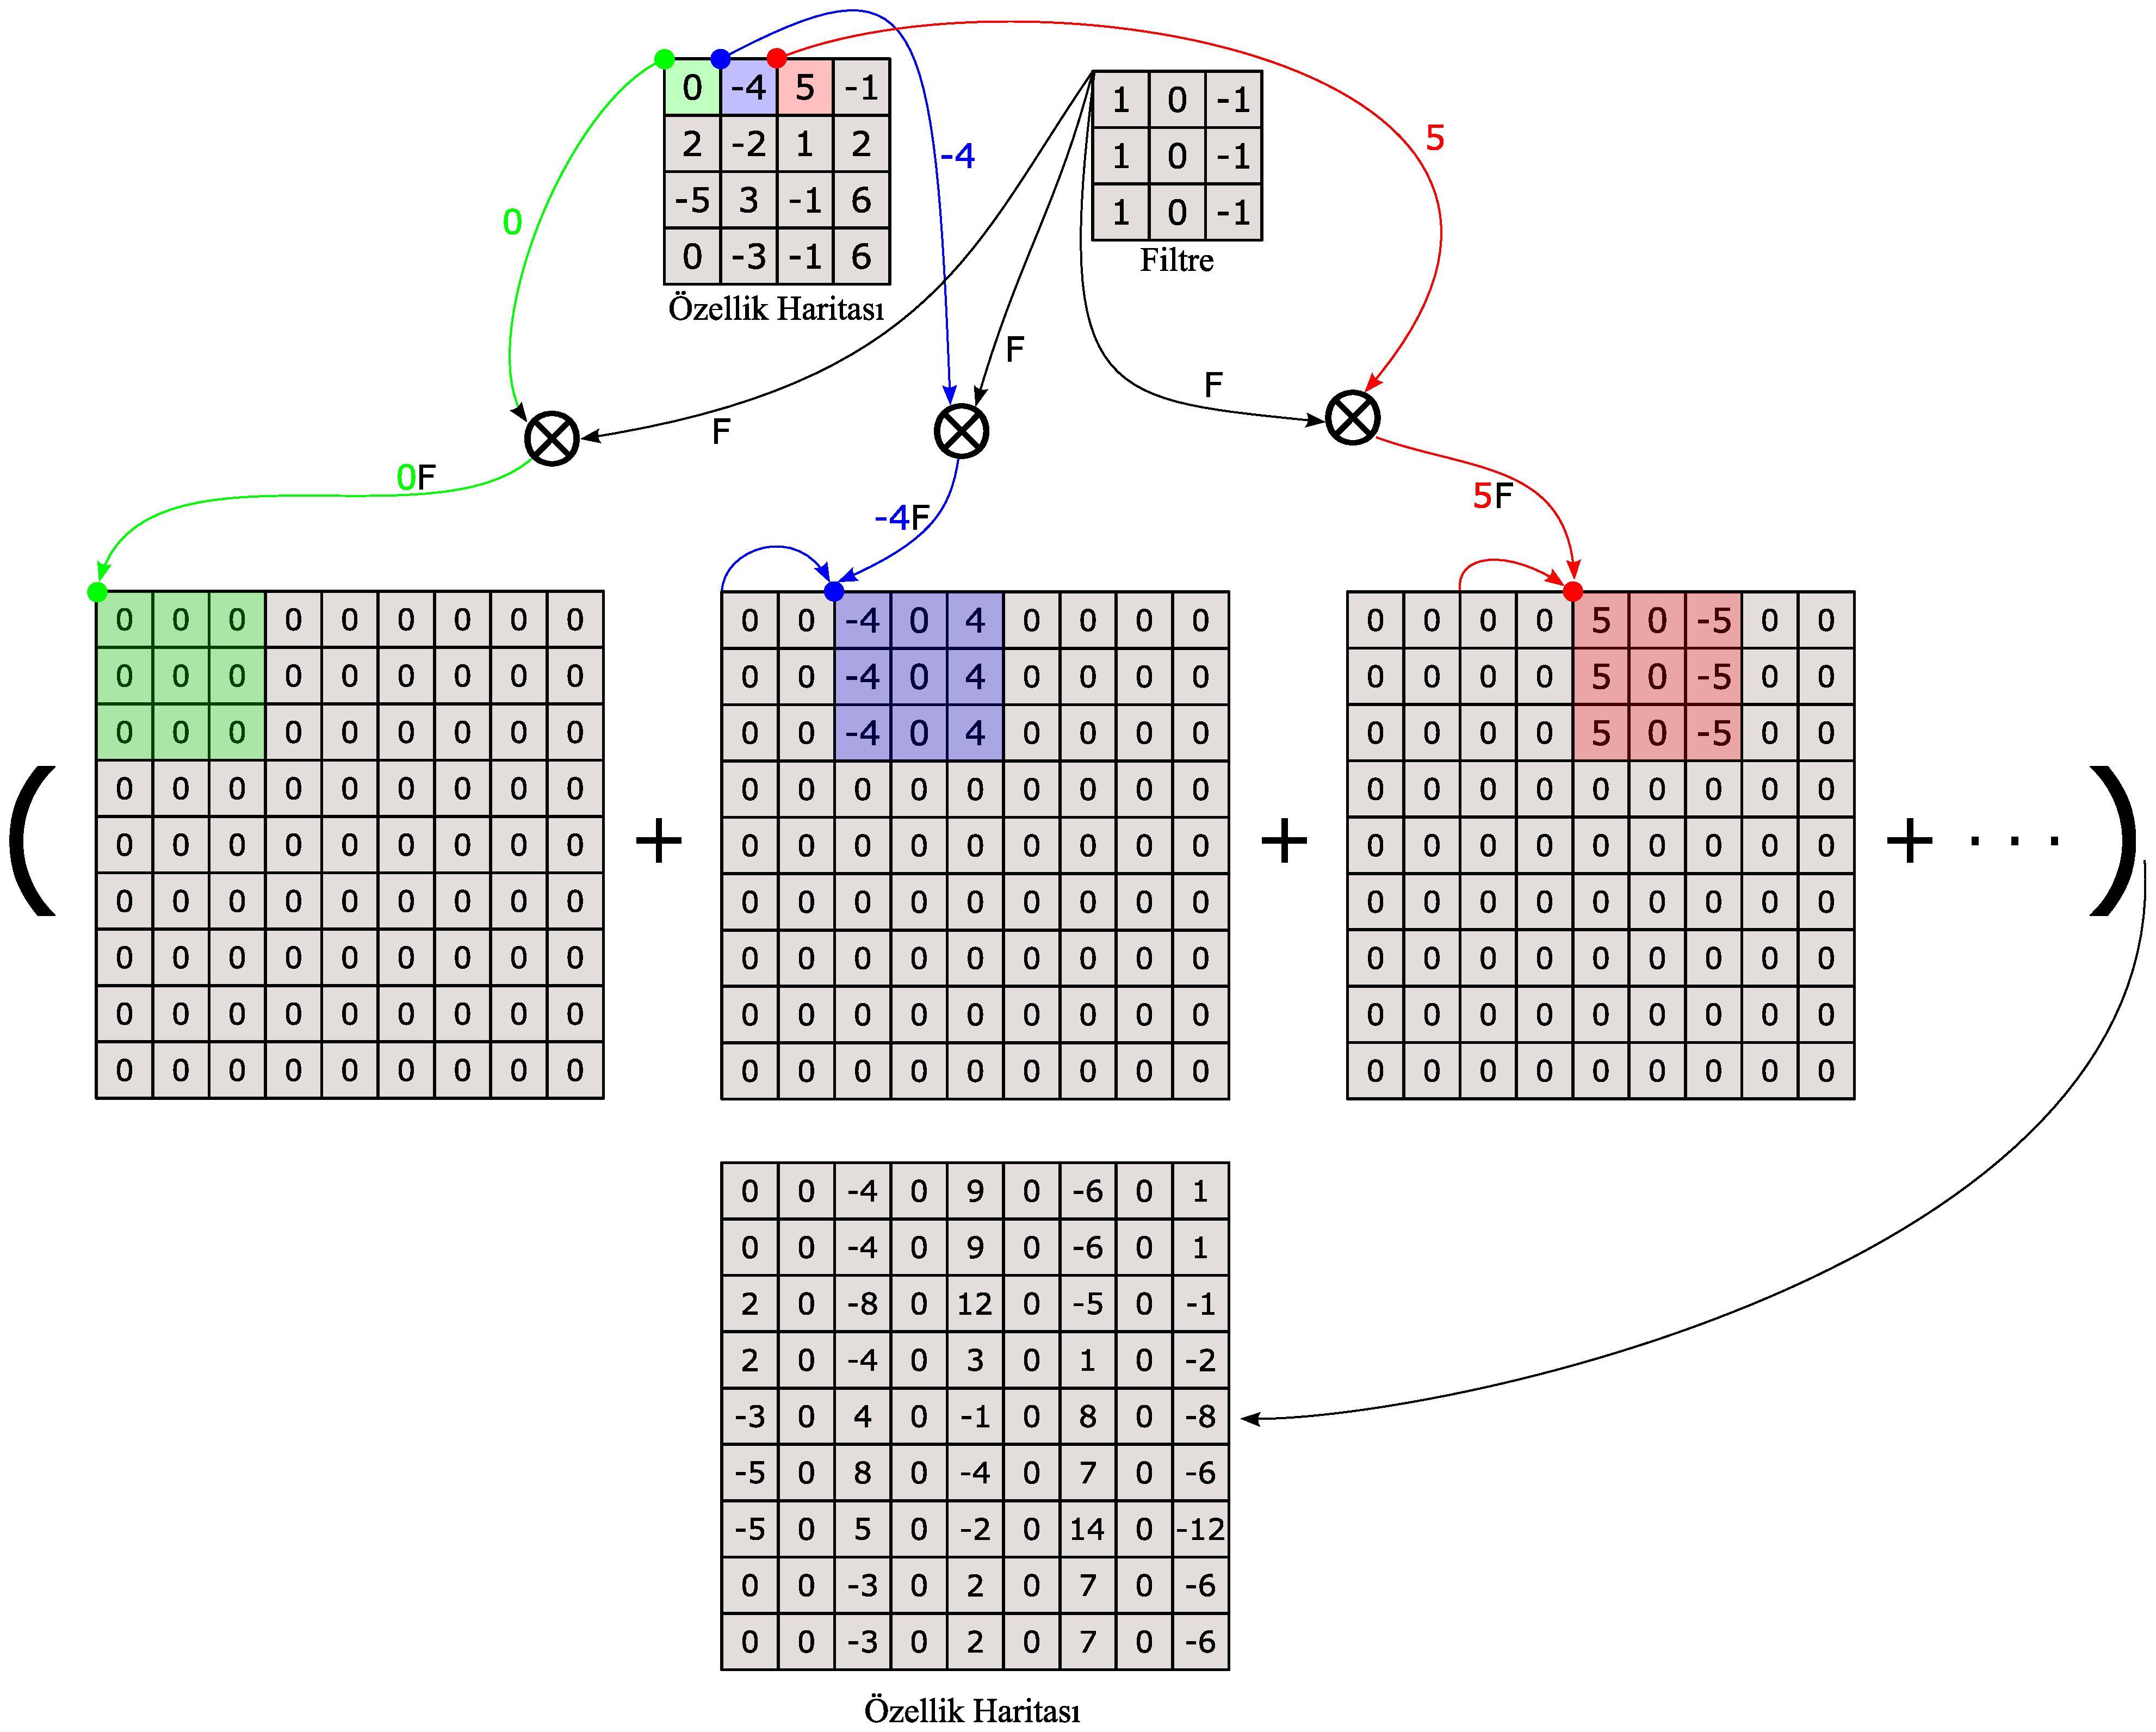
\includegraphics[scale=0.2]{Yapilan-Calismalar/Figures/conv2Dtranspose2.pdf}
		}
	\end{center}
\end{figure}

Ters konvolüsyon işleminde dolgulama konvolüsyon işleminin tersi mantığında çalışmaktadır. Eğer dolgulama miktarı $0$ olarak seçilirse Şekil \ref{fig:conv2Dtranspose1}'de görüldüğü gibi giriş görüntüsüne boyut artırma işlemi gerçekleştirilmektedir. Görüldüğü gibi boyut artırma miktarı Şekil \ref{fig:conv2d}'deki konvolüsyon işlemi öncesindeki giriş verisinin boyutlarına eşit olmaktadır. Bu özellik segmentasyon aşamasında ardışık özellik çıkarma aşamalarından sonra segmente edilmiş ve giriş görüntüsüyle eşit boyutlarda özellik haritaları elde etmemizi sağlamaktadır.

Ters konvolüsyon işleminde adım miktarının artırılması ise yine konvolüsyon işleminin ters yönünde boyutu artırmaktadır. Ters konvolüsyon işleminde adım miktarı konvolüsyon işleminde uygulanan adım miktarı ile eşdeğer seçilerek konvolüsyon işlemi ile kaybedilen özellik haritası ebatlarının geri kazanılmasını sağlayabilmektedir. Şekil \ref{fig:conv2Dtranspose2}'te görüldüğü gibi adım sayısının artırılması ters konvolüsyon işlemi sonrasında elde edilen özellik haritalarının ebatlarının büyümesini sağlamaktadır.

Dolgulama miktarı ise yine konvolüsyon işlemindeki dolgulamanın aksine kırpma işlemi gerçekleştirmektedir. Dolgulama miktarı konvolüsyon işleminde olduğu gibi Eşitlik \ref{eq:padding} kullanılarak hesaplanmaktadır. Hesaplanan dolgulama miktarı kadar pikseller Şekil \ref{fig:conv2Dtrpadding}'te gösterildiği gibi nihai ters konvolüsyon özellik haritasından kırpılmaktadır.

\captionsetup[figure]{margin={0.4cm,-0.2cm}}
\begin{figure}[h!]
	\begin{center}
		\vspace{0.4cm}
		\captionbox{2B konvolüsyon işleminde dolgulama.\label{fig:conv2Dtrpadding}}
		{
			\vspace{0.4cm}
			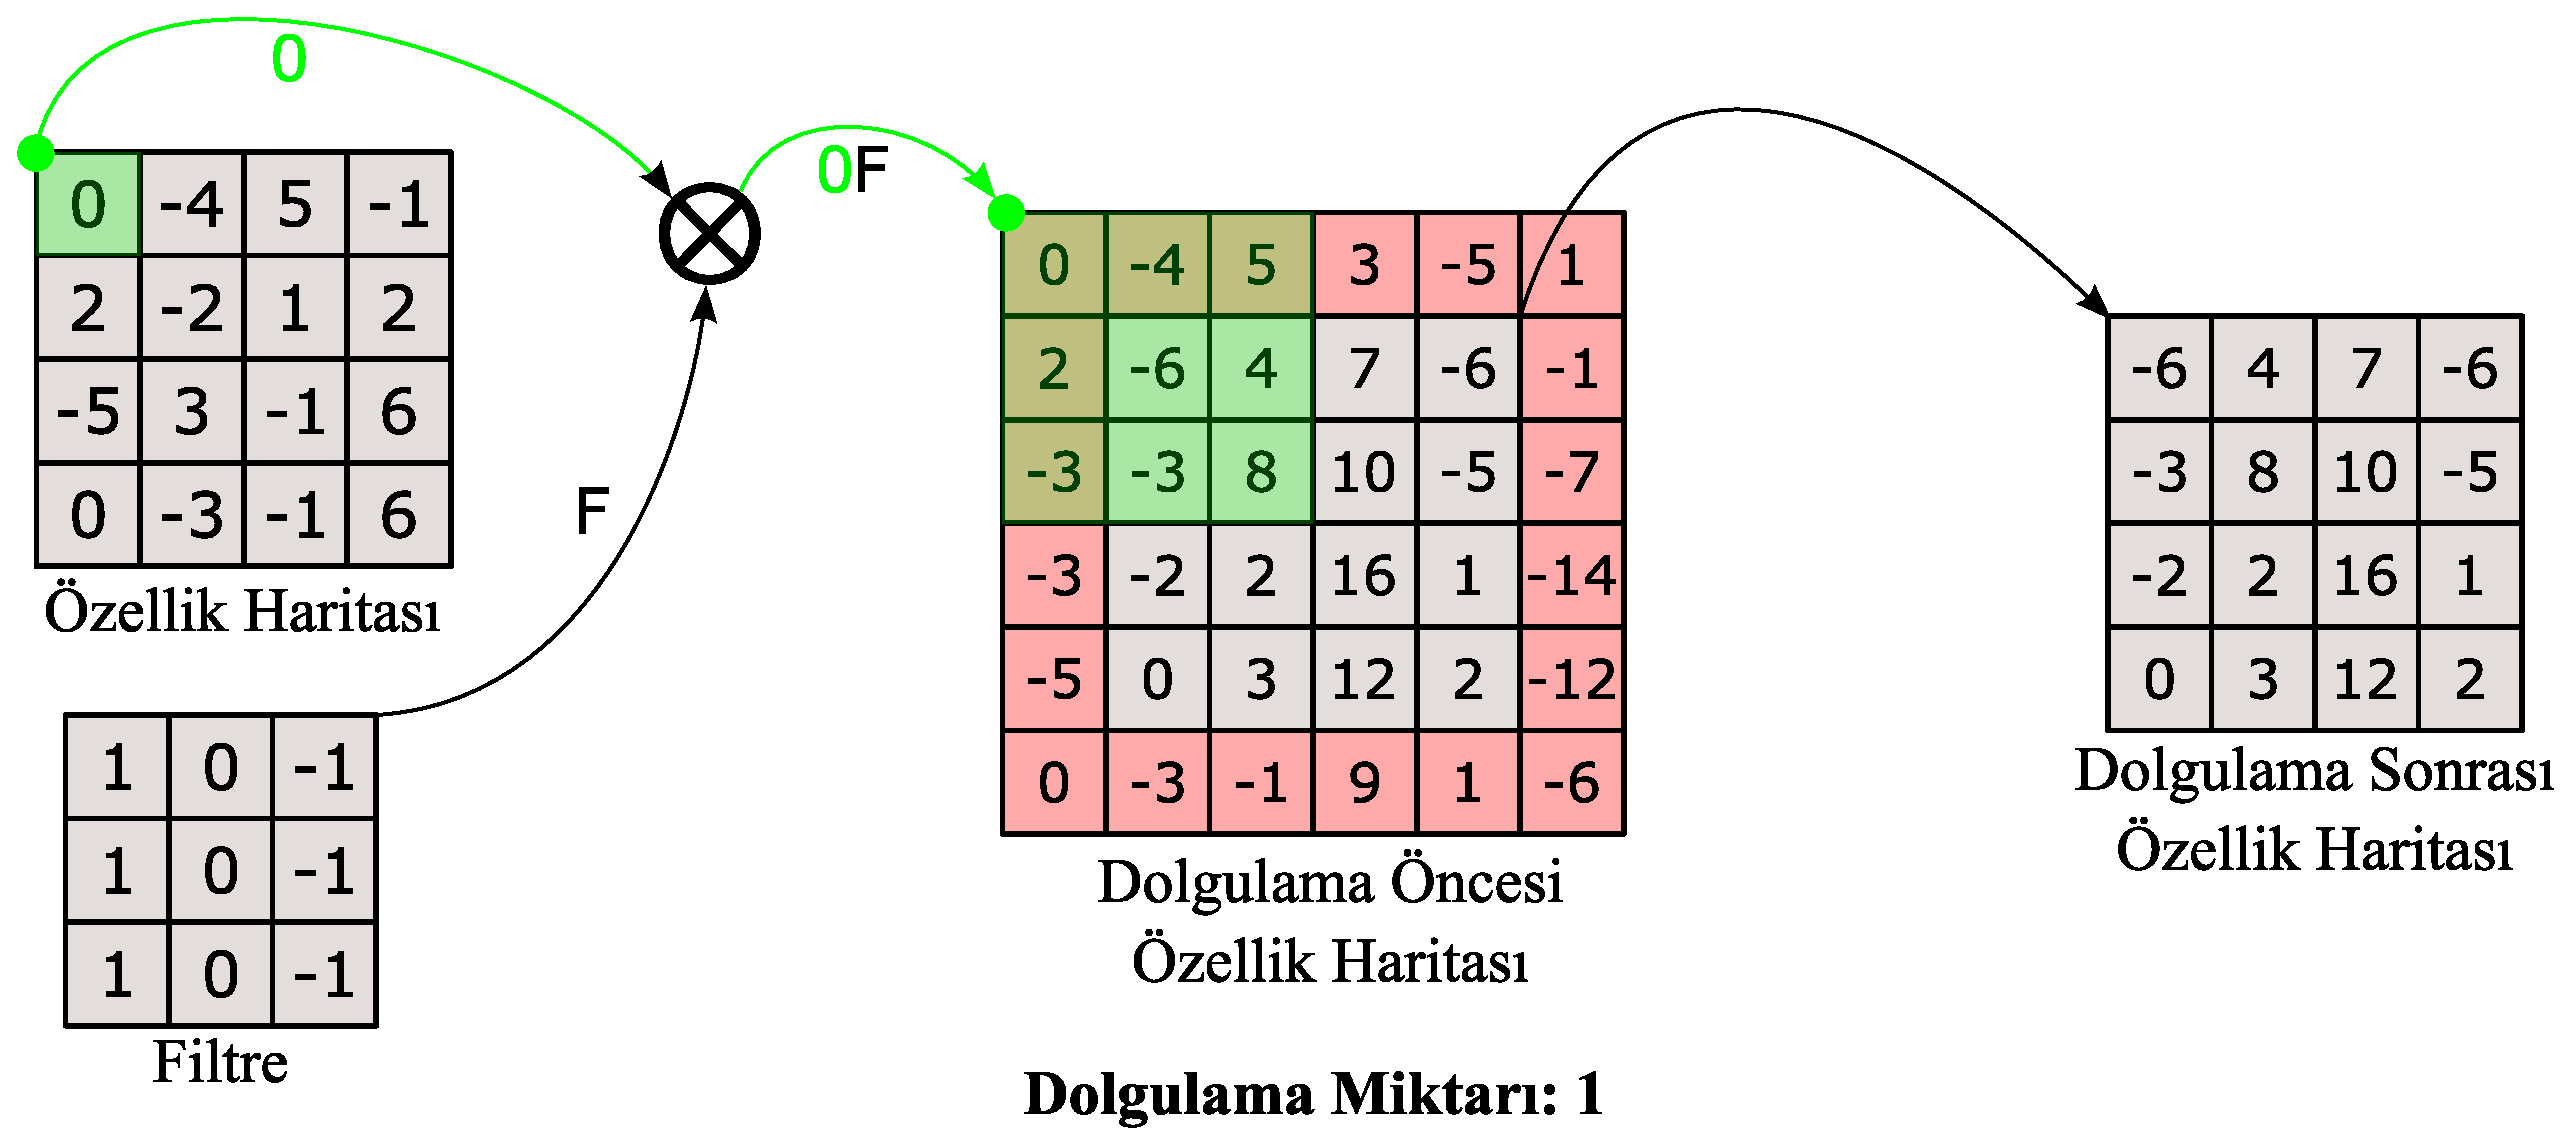
\includegraphics[scale=0.3]{Yapilan-Calismalar/Figures/conv2Dtrpadding.pdf}
		}
	\end{center}
\end{figure}

Ters konvolüsyon katmanlarının eğitimi konvolüsyon katmanlarına benzer şekilde gerçekleştirilmektedir. Konvolüsyon katmanında olduğu gibi girişine $G$ giriş verisi uygulanan $F$ eğitilebilir filtre parametrelerine sahip ters konvolüsyon katmanının çıkışı $O$ olmak üzere, $F$ filtre parametrelerini güncellemek için gerekli ağın genel hatasının gradyanının geri yayılım algoritmasının zincir kuralına göre Eşitlik \ref{eq:convFderivative}'den elde edilen kısmi türev ile gerçekleştirilmektedir. Ters konvolüsyon katmanından önceki katmanlara ise bu gradyan bilgisi Eşitlik \ref{eq:convGderivative} ile aktarılmaktadır.
 
\subsubsection{Aktivasyon Katmanları}
Aktivasyon katmanları eğitilebilir katmanların hemen ardından eklenerek peşine eklendiği katmanın doğrusallıktan kurtulmasını sağlamaktadır. Doğrusal bir öğrenme 2B hiperdüzlemde birinci dereceden bir eğri çizmeyi sağlayabilmektedir. Oysaki gerçek hayat problemlerini sınıflandırabilmek için doğrusal ayıraçlar kullanmak Şekil \ref{fig:lineer_nonlineer}'te görüldüğü gibi veriyi verimsiz sınıflandırmaya sebep olmaktadır.

\captionsetup[figure]{margin={0.4cm,-3cm}}
\begin{figure}[h!]
	\begin{center}
		\vspace{0.4cm}
		\captionbox{Doğrusal ve doğrusal olmayan aktivasyon fonksiyonları ile verinin sınıflandırılması.\label{fig:lineer_nonlineer}}
		{
			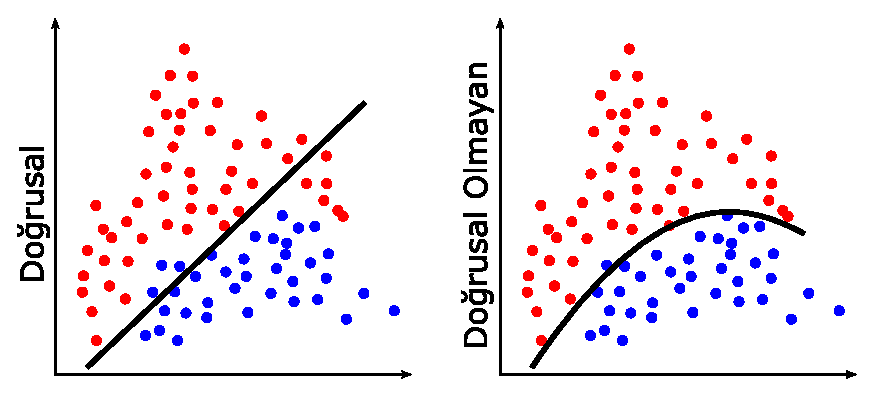
\includegraphics[scale=0.64]{Yapilan-Calismalar/Figures/lineer_nonlineer.pdf}
		}
	\end{center}
\end{figure}

Derin öğrenme modellerinde geri yayılım algoritması için gradyan tabanlı optimizasyon teknikleri kullanıldığından eğitim aşamasında zincir kuralına göre türevi kolay hesaplanabilen bir aktivasyon fonksiyonu tercih etmek hesaplama kolaylığı sağlamaktadır.
\vspace{0.2cm}

\begin{itemize}
    \item Doğrusal Aktivasyon Fonksiyonu:
    
    Doğrusal aktivasyon fonksiyonu ileri yönde hesaplama yapıldığında bir önceki katmandan gelen çıkış ifadesinin Eşitlik \ref{eq:lineer_activ}'te gösterildiği gibi değiştirilmeden kullanıldığı aktivasyon fonksiyonudur.
    {\setlength{\mathindent}{0cm}
    \begin{equation}
    	\label{eq:lineer_activ}
    	f(x)=O=x
    \end{equation}
    \vspace{-1.5cm}
    \begin{equation}
    	\label{eq:dlineer_activ}
    	f^{\prime}(x)=\frac{\partial L}{\partial  O}=1
    \end{equation}}    
    Doğrusal aktivasyon fonksiyonu Eşitlik \ref{eq:dlineer_activ}'te gösterildiği gibi türevi sabit (1 değerine eşit) bir aktivasyon fonksiyonudur. Doğrusal aktivasyon fonksiyonu ve doğrusal aktivasyon fonksiyonunun türevi Şekil \ref{fig:lineer_comb}'da gösterildiği gibidir.    
    \captionsetup[figure]{margin={0.3cm,-1cm}}
    \begin{figure}[h!]
    	\begin{center}
    		\vspace{0.4cm}
    		\captionbox{Doğrusal aktivasyon fonksiyonu ve türevi.\label{fig:lineer_comb}}
    		{
    			\vspace{0.4cm}
    			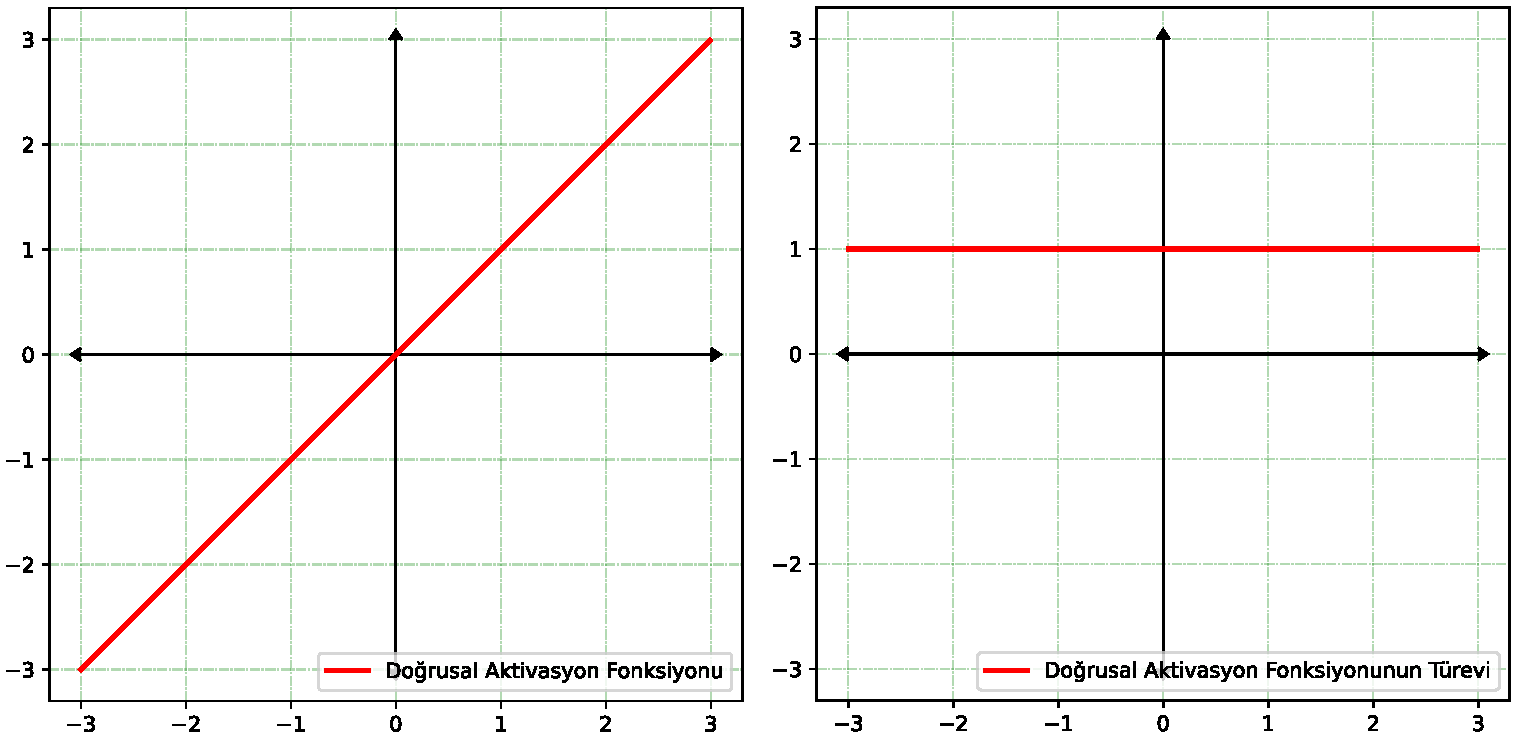
\includegraphics[scale=0.5]{Yapilan-Calismalar/Figures/lineer_comb.pdf}
    		}
    	\end{center}
    \end{figure}    
    Bu fonksiyonun türevinin sabit olması geri yayılım tekniği ile eğitim aşamasında çıkış ile giriş arasında bir ilişki kurulmasını mümkün kılmamaktadır. Ayrıca doğrusal aktivasyon fonksiyonu kullanıldığında doğrusal aktivasyon fonksiyonlarının kombinasyonları da doğrusal bir fonksiyon olduğundan katman sayısının da önemi ortadan kalkmaktadır. Bu durumda doğrusal aktivasyon fonksiyonları ile kurulan ardışıl katmanlar sanki tek bir katmanmış gibi davranmaktadırlar. Doğrusal aktivasyon fonksiyonu doğrusal kestirim modelleri kurmak için tercih edilen bir aktivasyon fonksiyonudur.
    
    \item Sigmoid Aktivasyon Fonksiyonu:
    
    Sigmoid aktivasyon fonksiyonu en tercih edilen aktivasyon fonksiyonlarından biridir. Türevinin kolay hesaplanabilir olması, monoton bir fonksiyon olması, yumuşak bir türevleme sunması gibi avantajları mevcuttur. Sigmoid aktivasyon fonksiyonu Eşitlik \ref{eq:sigmoid}, sigmoid aktivasyon fonksiyonunun türevi ise  Eşitlik \ref{eq:dsigmoid} kullanılarak hesaplanmaktadır.
    {\setlength{\mathindent}{0cm}
    \begin{equation}
    	\label{eq:sigmoid}
    	f(x)=O = \frac{1}{1+e^{-x}}
    \end{equation}
    \vspace{-1cm}
    \begin{equation}
    	\label{eq:dsigmoid}
    	f^{\prime}(x)= \frac{\partial L}{\partial  O}=O(1-O)
    \end{equation}}   
    Sigmoid aktivasyon fonksiyonu ve sigmoid aktivasyon fonksiyonunun türevi Şekil \ref{fig:sigmoid_comb}'de gösterilmektedir. Sigmoid aktivasyon fonksiyonu $[0 - 1]$ aralığında değer üretmektedir. Giriş $x$ değeri büyüdükçe yada küçüldükçe ani bir şekilde $0$ yada $1$'e yakınsadığı için sonucun net üretilebilmesini sağlamaktadır.
    
    \captionsetup[figure]{margin={0.3cm,-1cm}}
    \begin{figure}[h!]
    	\begin{center}
    		\vspace{0.4cm}
    		\captionbox{Sigmoid aktivasyon fonksiyonu ve türevi.\label{fig:sigmoid_comb}}
    		{
    			\vspace{0.4cm}
    			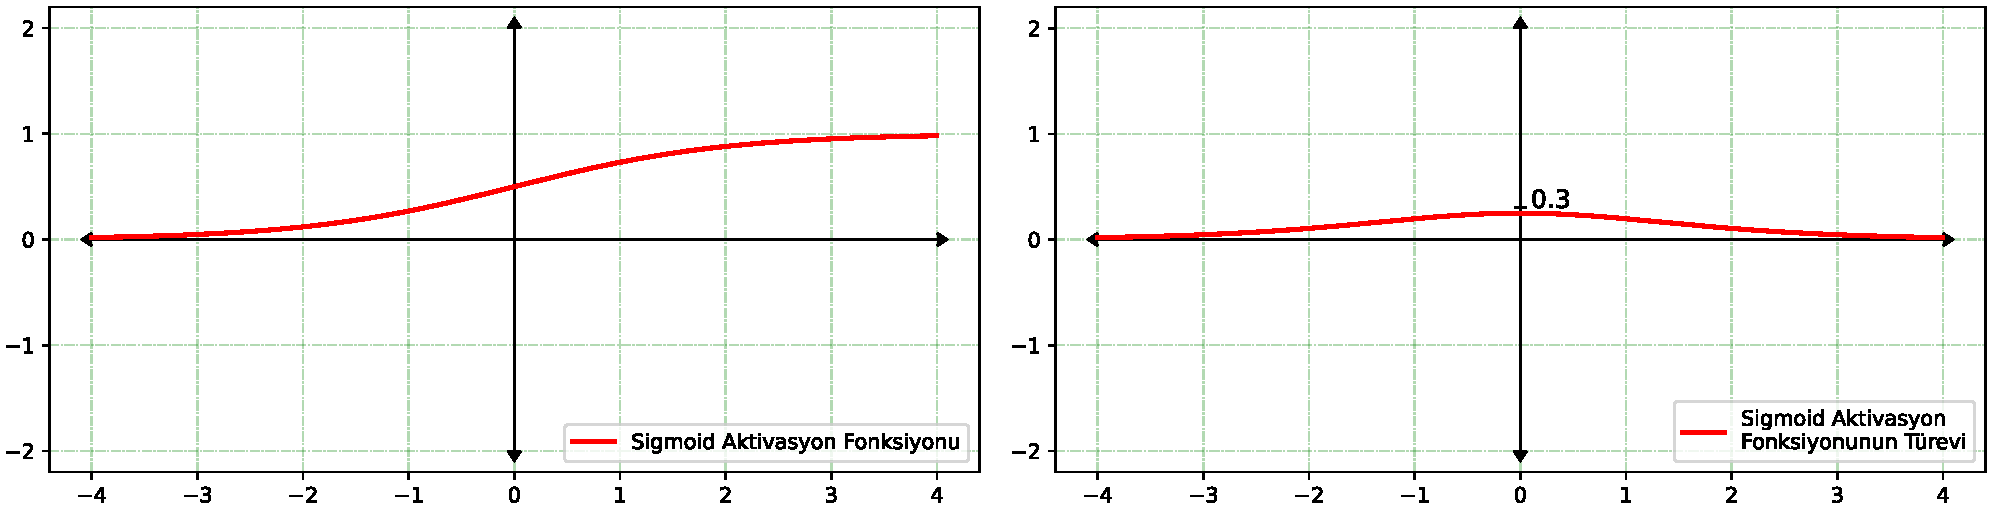
\includegraphics[scale=0.45]{Yapilan-Calismalar/Figures/sigmoid_comb.pdf}
    		}
    	\end{center}
    \end{figure}
    
    Katman sayısı arttıkça eğitim aşamasında sıfıra çok yakın türevler elde edilmekte ve dolayısıyla Kaybolan Eğim (Vanishing Gradient) problemi ile karşılaşılmaktadır \cite{hochreiter1998vanishing}. Tahmin merkezi sıfırın üzerinde olmaması ve katman sayısı arttıkça hesaplama maliyetinin artması sigmoid aktivasyon fonksiyonunun popülerliğini düşürmektedir. Genellikle çıkış katman aktivasyon fonksiyonu olarak tercih edilmektedir. Çıkış katmanı olarak Sigmoid aktivasyon fonksiyonu tercih edildiğinde eğitim veri seti $[0-1]$ aralığına uygun şekilde hazırlanmalıdır.
    
    \item Hiperbolik Tanjant Aktivasyon Fonksiyonu:
    
    Sigmoid aktivasyon fonksiyonuna oldukça benzer bir aktivasyon fonksiyonudur. Sigmoid aktivasyon fonksiyonundan en temel farklılığı $[-1,+1]$ aralığında değer üretmesinden dolayı sıfır merkezcil bir aktivasyon fonksiyonu oluşudur. Ayrıca sigmoid aktivasyon fonksiyonuna göre hiperbolik tanjant aktivasyon fonksiyonunun türevi Şekil \ref{fig:tanh_comb}'de gösterildiği gibi daha geniş aralıkta değerler alabilmektedir. Hiperbolik tanjant aktivasyon fonksiyonu Eşitlik \ref{eq:tanh}'de, hiperbolik tanjant aktivasyon fonksiyonunun türevi ise  Eşitlik \ref{eq:dtanh}'da verildiği gibi hesaplanmaktadır.
    {\setlength{\mathindent}{0cm}
    \begin{equation}
    	\label{eq:tanh}
    	f(x)=O=\frac{(e^{x} - e^{-x})}{(e^{x} - e^{-x})}
    \end{equation}
    \vspace{-1cm}
    \begin{equation}
    	\label{eq:dtanh}
    	f^{\prime}(x)= \frac{\partial L}{\partial  O} =1-O^{2}
    \end{equation}}    
    \captionsetup[figure]{margin={0.3cm,-1cm}}
    \begin{figure}[h!]
    	\begin{center}
    		\vspace{-0.6cm}
    		\captionbox{Hiperbolik tanjant aktivasyon fonksiyonu ve türevi.\label{fig:tanh_comb}}
    		{
    			\vspace{0.4cm}
    			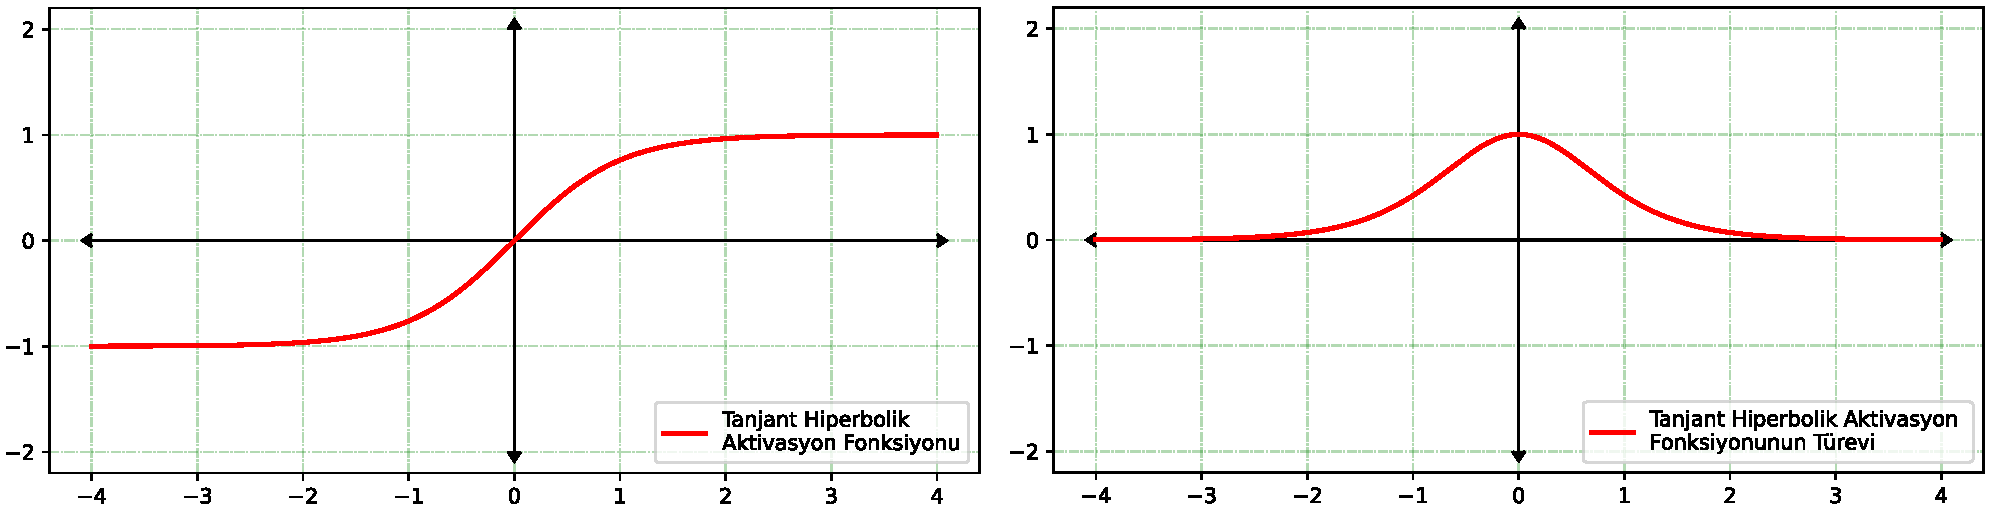
\includegraphics[scale=0.45]{Yapilan-Calismalar/Figures/tanh_comb.pdf}
    		}
    	\end{center}
    \end{figure}  
    
    \vspace{-0.6cm}
    Hiperbolik tanjant aktivasyon fonksiyonu, sigmoid aktivasyon fonksiyonunda olduğu gibi kaybolan eğim ve hesaplama maliyetinin yüksek olması gibi dezavantajlara sahiptir. Bu sebeplerden dolayı genellikle son katman aktivasyon fonksiyonu olarak tercih edilmektedir.
    
    \item ReLU Benzeri Aktivasyon Fonksiyonları:
    
    Doğrultulmuş Doğrusal Birim (Rectified Linear Unit - ReLU) aktivasyon fonksiyonu çok katmanlı mimarilerde kaybolan eğim (vanishing gradient) problemine çözüm olarak kullanılmaya başlanan bir aktivasyon fonksiyonudur \cite{hochreiter1998vanishing}. ReLU aktivasyon fonksiyonu Eşitlik \ref{eq:relu}, ReLU aktivasyon fonksiyonunun türevi ise  Eşitlik \ref{eq:drelu} kullanılarak hesaplanmaktadır.
    {\setlength{\mathindent}{0cm}
    \begin{equation}
    	\label{eq:relu}
    	f(x)= O = \left\{\begin{array}{ll}
    		0 & \text { for } x<0 \\
    		x & \text { for } x \geq 0
    	\end{array}\right.
    \end{equation}
    \vspace{-1cm}
    \begin{equation}
    	\label{eq:drelu}
    	f^{\prime}(x)= \frac{\partial L}{\partial  O} = \left\{\begin{array}{ll}
    		0 & \text { for } x<0 \\
    		1 & \text { for } x \geq 0
    	\end{array}\right.
    \end{equation}}    
    Şekil \ref{fig:relu_comb}'da gösterildiği gibi ReLU aktivasyon fonksiyonu $[0,+\infty]$ aralığında çıkış değeri üretebilmekte ve negatif değerler için $0$, pozitif değerler için $1$ türevini sağlamaktadır. ReLU aktivasyon fonksiyonu sigmoid ve hiperbolik tanjant aktivasyonunun aksine negatif eksende $0$ değerini üretmesinden ve ileri yönlü hesaplamada $0$ çıkışlı algılayıcıların tetiklenmemesinden dolayı çok daha düşük hesaplama maliyetine sahiptir. Doğrusal bir aktivasyon fonksiyonuna ne kadar benzese de aslında doğrusal olmayan bir aktivasyon fonksiyonudur. Bu fonksiyon farklı aktivasyon fonksiyonları ile birlikte birleştirilerek kullanılabilmektedir.
    
    \captionsetup[figure]{margin={0.3cm,-1cm}}
    \begin{figure}[h!]
    	\begin{center}
    		\vspace{0.4cm}
    		\captionbox{ReLU benzeri aktivasyon fonksiyonları ve bu  fonksiyonların türevleri.\label{fig:relu_comb}}
    		{
    			\vspace{0.4cm}
    			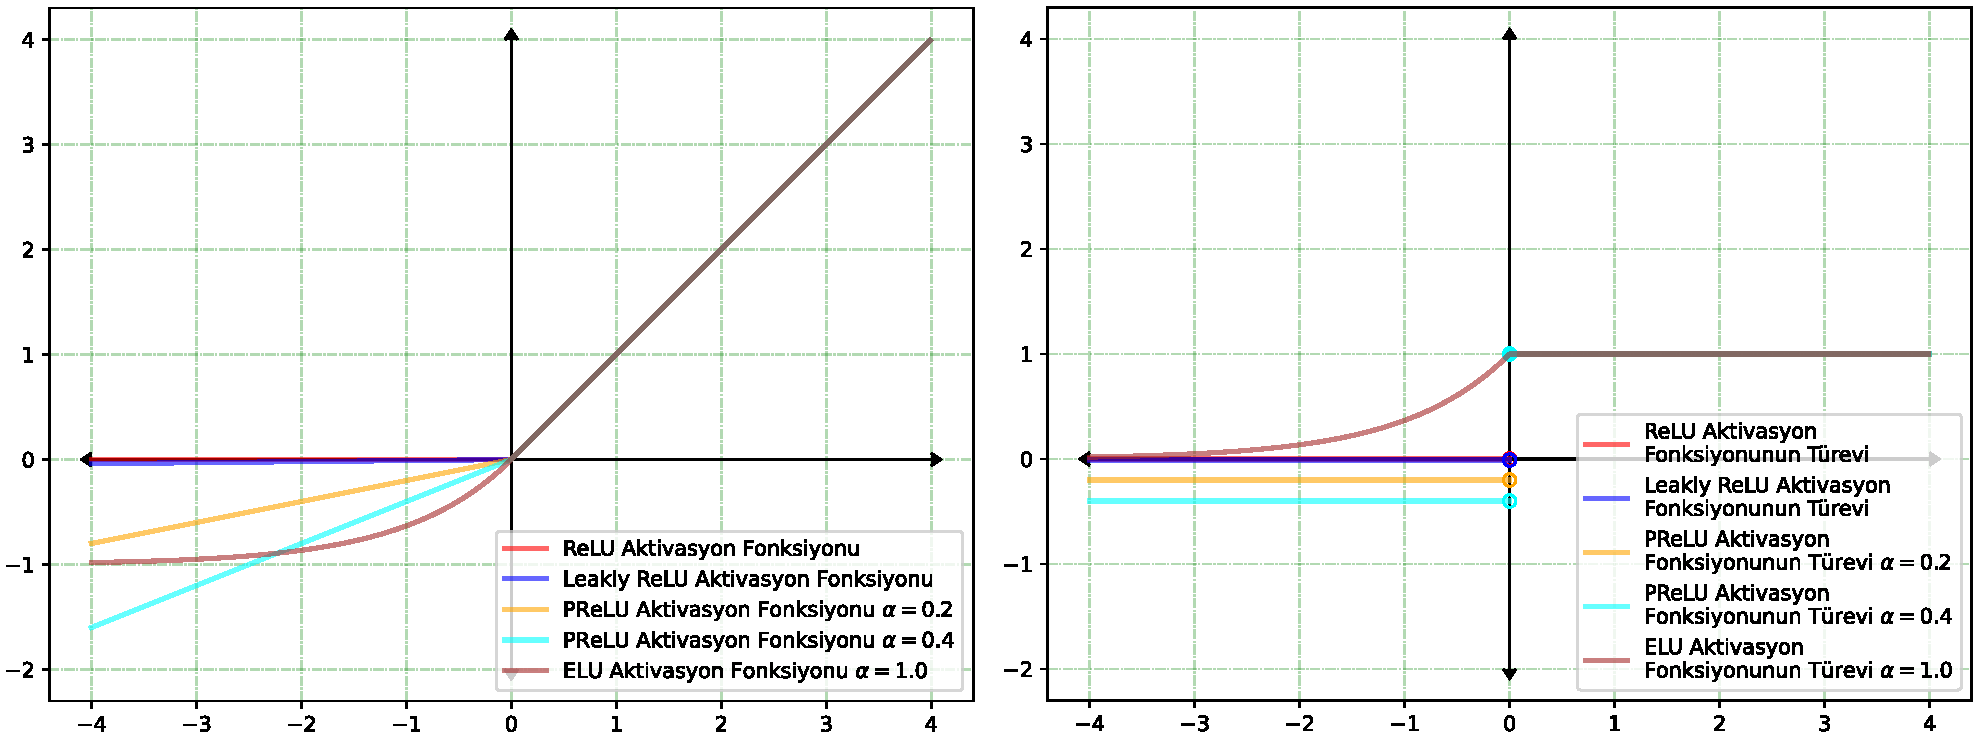
\includegraphics[scale=0.45]{Yapilan-Calismalar/Figures/relu_comb.pdf}
    		}
    	\end{center}
    \end{figure}
    
    ReLU aktivasyon fonksiyonu girişinden $0$ yada sıfırın altında değer geldiğinde sürekli $0$ çıkışını üretmektedir. Bu durum Ölen ReLU Problemi (The Dying ReLU Problem) adı verilen, eğitimin gerçekleşmediği katmanların ortaya çıkmasına sebebiyet vermektedir. Bundan dolayı ReLU aktivasyon fonksiyonu güncellenerek Sızan ReLU (Leaky ReLU), Parametrik ReLU (Parametric ReLU - PReLU), Eksponansiyel Doğrusal Birim (Exponential Linear Unit - ELU) gibi aktivasyon fonksiyonları ortaya çıkarılmıştır.
    
    \begin{itemize}
    	\item Leaky ReLU aktivasyon fonksiyonu ReLU aktivasyon fonksiyonundan farklı olarak $0$'dan küçük değerler için de değerler üretilebilmesini sağlamaktadır. Leaky ReLU aktivasyon fonksiyonu Eşitlik \ref{eq:lrelu}, ReLU aktivasyon fonksiyonunun türevi ise  Eşitlik \ref{eq:dlrelu}'teki gibi hesaplanmaktadır. 
    	{\setlength{\mathindent}{-1cm}
    	\begin{equation}
    		\label{eq:lrelu}
    		f(x)= O = \left\{\begin{array}{ll}
    			0.01x & \text { for } x<0 \\
    			x & \text { for } x \geq 0
    		\end{array}\right.
    	\end{equation}
    	\vspace{-1cm}
    	\begin{equation}
    		\label{eq:dlrelu}
    		f^{\prime}(x)= \frac{\partial L}{\partial  O} =\left\{\begin{array}{ll}
    			0.01 & \text { for } x<0 \\
    			1 & \text { for } x \geq 0
    		\end{array}\right.
    	\end{equation}}
    	\item PReLU aktivasyon fonksiyonu Leaky ReLU aktivasyon fonksiyonunun geliştirilmiş versiyonudur. Leaky ReLU aktivasyon fonksiyonunda $0$'dan küçük değerler $0.01$ sabit katsayısı ile çarpılırken, PReLU aktivasyon fonksiyonunda bu değerin $\alpha$ parametresi ile değiştirilebilir olması sağlanmaktadır. PReLU aktivasyon fonksiyonu Eşitlik \ref{eq:prelu}, ReLU aktivasyon fonksiyonunun türevi ise Eşitlik \ref{eq:dprelu}'te verildiği gibi hesaplanmaktadır.
    	{\setlength{\mathindent}{-1cm}
    	\begin{equation}
    		\label{eq:prelu}
    		f(x)= O =\left\{\begin{array}{ll}
    			\alpha x & \text { for } x<0 \\
    			x & \text { for } x \geq 0
    		\end{array}\right.
    	\end{equation}
    	\vspace{-1cm}
    	\begin{equation}
    		\label{eq:dprelu}
    		f^{\prime}(x)= \frac{\partial L}{\partial  O} = \left\{\begin{array}{ll}
    			\alpha & \text { for } x<0 \\
    			1 & \text { for } x \geq 0
    		\end{array}\right.
    	\end{equation}}
    	\item ELU aktivasyon fonksiyonu $0$'dan küçük değerler için $\alpha$ parametre değerine göre doğrusal olmayan değerler üretilebilmesini sağlamaktadır. ELU aktivasyon fonksiyonu Eşitlik \ref{eq:elu}, ReLU aktivasyon fonksiyonunun türevi ise Eşitlik \ref{eq:delu}'de gösterildiği gibi hesaplanmaktadır.
    	{\setlength{\mathindent}{-1cm}
    	\begin{equation}
    		\label{eq:elu}
    		f(x)= O = \left\{\begin{array}{ll}
    			\alpha(e^{x}-1) & \text { for } x<0 \\
    			x & \text { for } x \geq 0
    		\end{array}\right.
    	\end{equation}
    	\vspace{-1cm}
    	\begin{equation}
    		\label{eq:delu}
    		f^{\prime}(x)= \frac{\partial L}{\partial  O} =\left\{\begin{array}{ll}
    			\alpha e^{x} & \text { for } x<0 \\
    			O+\alpha & \text { for } x \geq 0
    		\end{array}\right.
    	\end{equation}}
    \end{itemize}
    
    \item Softmax Aktivasyon Fonksiyonu:
    
    Çok sınıflı sınıflandırma ihtiyacı doğrultusunda ortaya çıkarılmış bir aktivasyon fonksiyonudur. Softmax aktivasyon fonksiyonu haricindeki diğer tüm aktivasyon fonksiyonları iki sınıflı sınıflandırma aktivasyon fonksiyonlarıdır. Bu aktivasyon fonksiyonunun çıkış katmanındaki herbir algılayıcı çıkışı için sınıf sayısı uzunluğunda vektör oluşturulmaktadır. İleri yönde hesaplamada bu vektörün maksimum değerli indisleri girişten gelen verinin hangi sınıfa dahil olduğunu göstermektedir. Bu vektörün uzunluğu $n$ olarak kabul edilirse, $i$ inci indeksteki çıkış değeri $i$ sınıfı temsil etmek üzere Eşitlik \ref{eq:softmax}'deki gibi hesaplanmaktadır. Softmax fonksiyonunun türevi hesaplanırken, aslında tüm birinci dereceden kısmi türevlerin matrisi olan Jacobian matrisinin hesaplanması gerekmektedir. Eşitlik \ref{eq:dsoftmax}'da softmax aktivasyon fonksiyonunun türevi gösterilmektedir.
    {\setlength{\mathindent}{0cm}
    \begin{equation}
    	\label{eq:softmax}
    	f_{i}(\vec{x})= O_{i} =\frac{e^{x_{i}}}{\sum_{j=1}^{n} e^{x_{j}}} \quad \text { , } \quad \forall i=1, \ldots, n
    \end{equation}
    \vspace{-1cm}
    \begin{equation}
    	\label{eq:dsoftmax}
    	f^{\prime}_{i}(\vec{x})= \frac{\partial L}{\partial  O_{i}} = O_{i}(1\left\{i=j\right\}-O_{j}) \quad \text { , } \quad \forall i=1, \ldots, n \quad \text { , } \quad \forall j=1, \ldots, n
    \end{equation}}
    Softmax aktivasyon fonksiyonu sadece çıkış katmanında tercih edilen bir aktivasyon fonksiyonudur. 
\end{itemize}

\subsubsection{Yukarı Örnekleme Katmanları}
Yukarı örnekleme (Up Sampling) katmanları ters konvolüsyon katmanları gibi boyut artırma işlemi için tercih edilebilecek katmanlardandır. Yukarı örnekleme katmanları girişten uygulanan $G$ özellik haritasına interpolasyon teknikleri uygulayarak daha büyük ebatlarda çıkış $O$ özellik haritaları elde edilmesini sağlamaktadır. Yukarı örnekleme katmanlarında ters konvolüsyon katmanlarının aksine eğitilebilir parametre bulunmamaktadır. Bu sebeple yukarı örnekleme katmanları ardından dolgulama gerçekleştirilmiş konvolüsyon katmanları eklenerek eğitilebilir bloklar üretilebilmektedir \cite{dumoulin2016guide}. Yukarı örnekleme katmanları ardından konvolüsyon katmanları kullanılmaması durumunda eğitim olumsuz etkilenmektedir.

\subsubsection{Havuzlama Katmanları}
Havuzlama katmanı eğitilebilir parametresi bulunmayan katmanlardandır. Genellikle hesaplama maliyetini düşürmek ve konvolüsyon katmanlarından sonra boyut azaltma işlemi için tercih edilmektedirler. Bir anlamda konvolüsyon katmanlarından elde edilen özellik haritalarının özetlenmesi işlemini gerçekleştirmektedirler. Böylece çıkarılan özellikler konumsal değişimlere daha dayanıklı hale getirilmiş olmaktadırlar. Havuzlama uygulanacak özellik haritasının havuzlama bölgesi $P$ ve $P$'nin alt havuzlama bölgesi $E$ Eşitlik \ref{eq:pooling1}'da gösterildiği gibi temsil edilmektedir.
\begin{equation}
	\label{eq:pooling1}
	E_{P} = \left\{ e_{k} \mid k \in P \right\}
\end{equation}
    
Literatürde birçok havuzlama tekniği olmakla birlikte genellikle maksimum havuzlama ve ortalama havuzlama yöntemleri tercih edilmektedir. Maksimum havuzlamada $P$ havuzlama bölgesinin $E_{P}$ alt havuzlama bölgesinde Eşitlik \ref{eq:maxpooling}'deki gibi maksimum değerli değeri seçilirken, ortalama havuzlamada $E_{P}$ alt bölgesinin Eşitlik \ref{eq:meanpooling}'deki gibi değerlerinin ortalaması hesaplanarak bu ortalama değerleri kullanılmaktadır.
\begin{equation}
	\label{eq:maxpooling}
	P_{maksimum} = maksimum(E_{P})
\end{equation}
\vspace{-1cm}
\begin{equation}
	\label{eq:meanpooling}
	P_{ortalama} = \frac{\sum E_{P}}{\left| E_{P} \right|}
\end{equation}

\captionsetup[figure]{margin={0.3cm,-3.2cm}}
\begin{figure}[h!]
	\begin{center}
		\vspace{0.4cm}
		\captionbox{Maksimum ve Ortalama havuzlama tekniklerinin $4 \times 4$ boyutuna sahip özellik haritasına uygulanması.\label{fig:pooling}}
		{
			\vspace{0.4cm}
			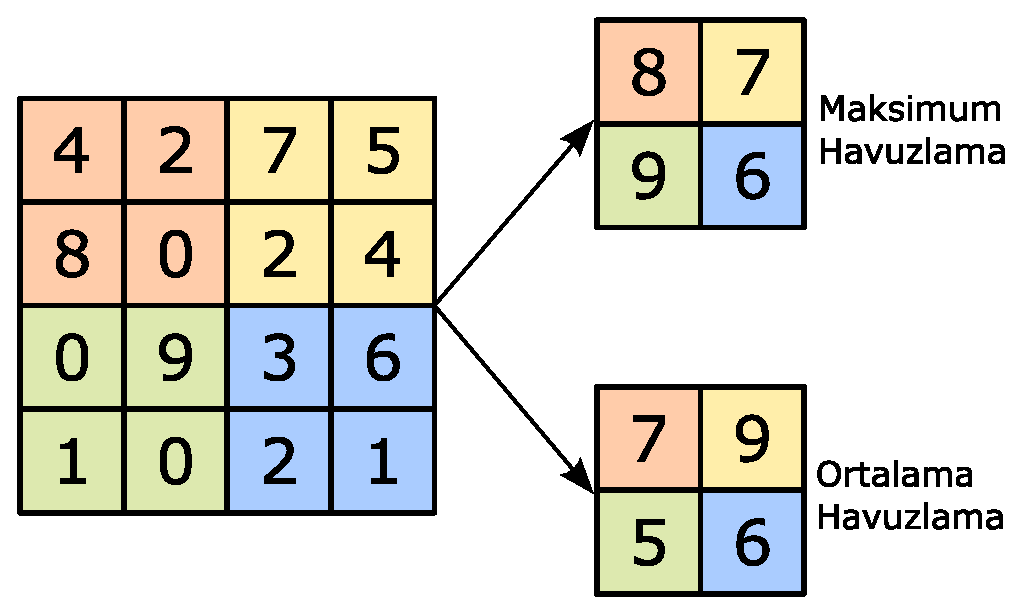
\includegraphics[scale=0.5]{Yapilan-Calismalar/Figures/pooling.pdf}
		}
	\end{center}
\end{figure}

Maksimum ve ortalama havuzlama tekniklerinde havuzlama miktarı $p=2 \times 2$, adım kaydırma miktarı $s=2$ seçildiğinde, bu havuzlama tekniklerinin $4 \times 4$ boyutuna sahip özellik haritasına uygulanması Şekil \ref{fig:pooling}'de gösterildiği gibi olmaktadır.

Havuzlama katmanı girişine uygulanan $G$ özellik haritasının havuzlama işlemi sonrası elde edilen çıkış özellik haritasının $O$ ebatları Eşitlik \ref{eq:poolingsize}'teki gibi hesaplanabilmektedir. 
\begin{equation}
	\label{eq:poolingsize}
	O=\left\lfloor \frac{G-p}{s} \right\rfloor+1
\end{equation}

\subsubsection{Birleştirme Katmanları}
Birleştirme katmanı, iki farklı katmanın çıkışı olan özellik haritalarının birleştirilmesinde kullanılmaktadır. İki farklı katmanın çıkışı olan özellik haritalarının birleştirilebilmesi için özellik haritalarının ebatlarının aynı olması gerekmektedir. Birleştirilecek özellik haritası sayısının farklı ve aynı sayıda olması durumları için iki farklı birleştirme yöntemi mevcuttur.

\captionsetup[figure]{margin={0.4cm,-1cm}}
\begin{figure}[h!]
	\begin{center}
		\vspace{0.4cm}
		\captionbox{Derinlik birleştirme işlemi (Concatenate).\label{fig:concatenate}}
		{
			\vspace{0.4cm}
			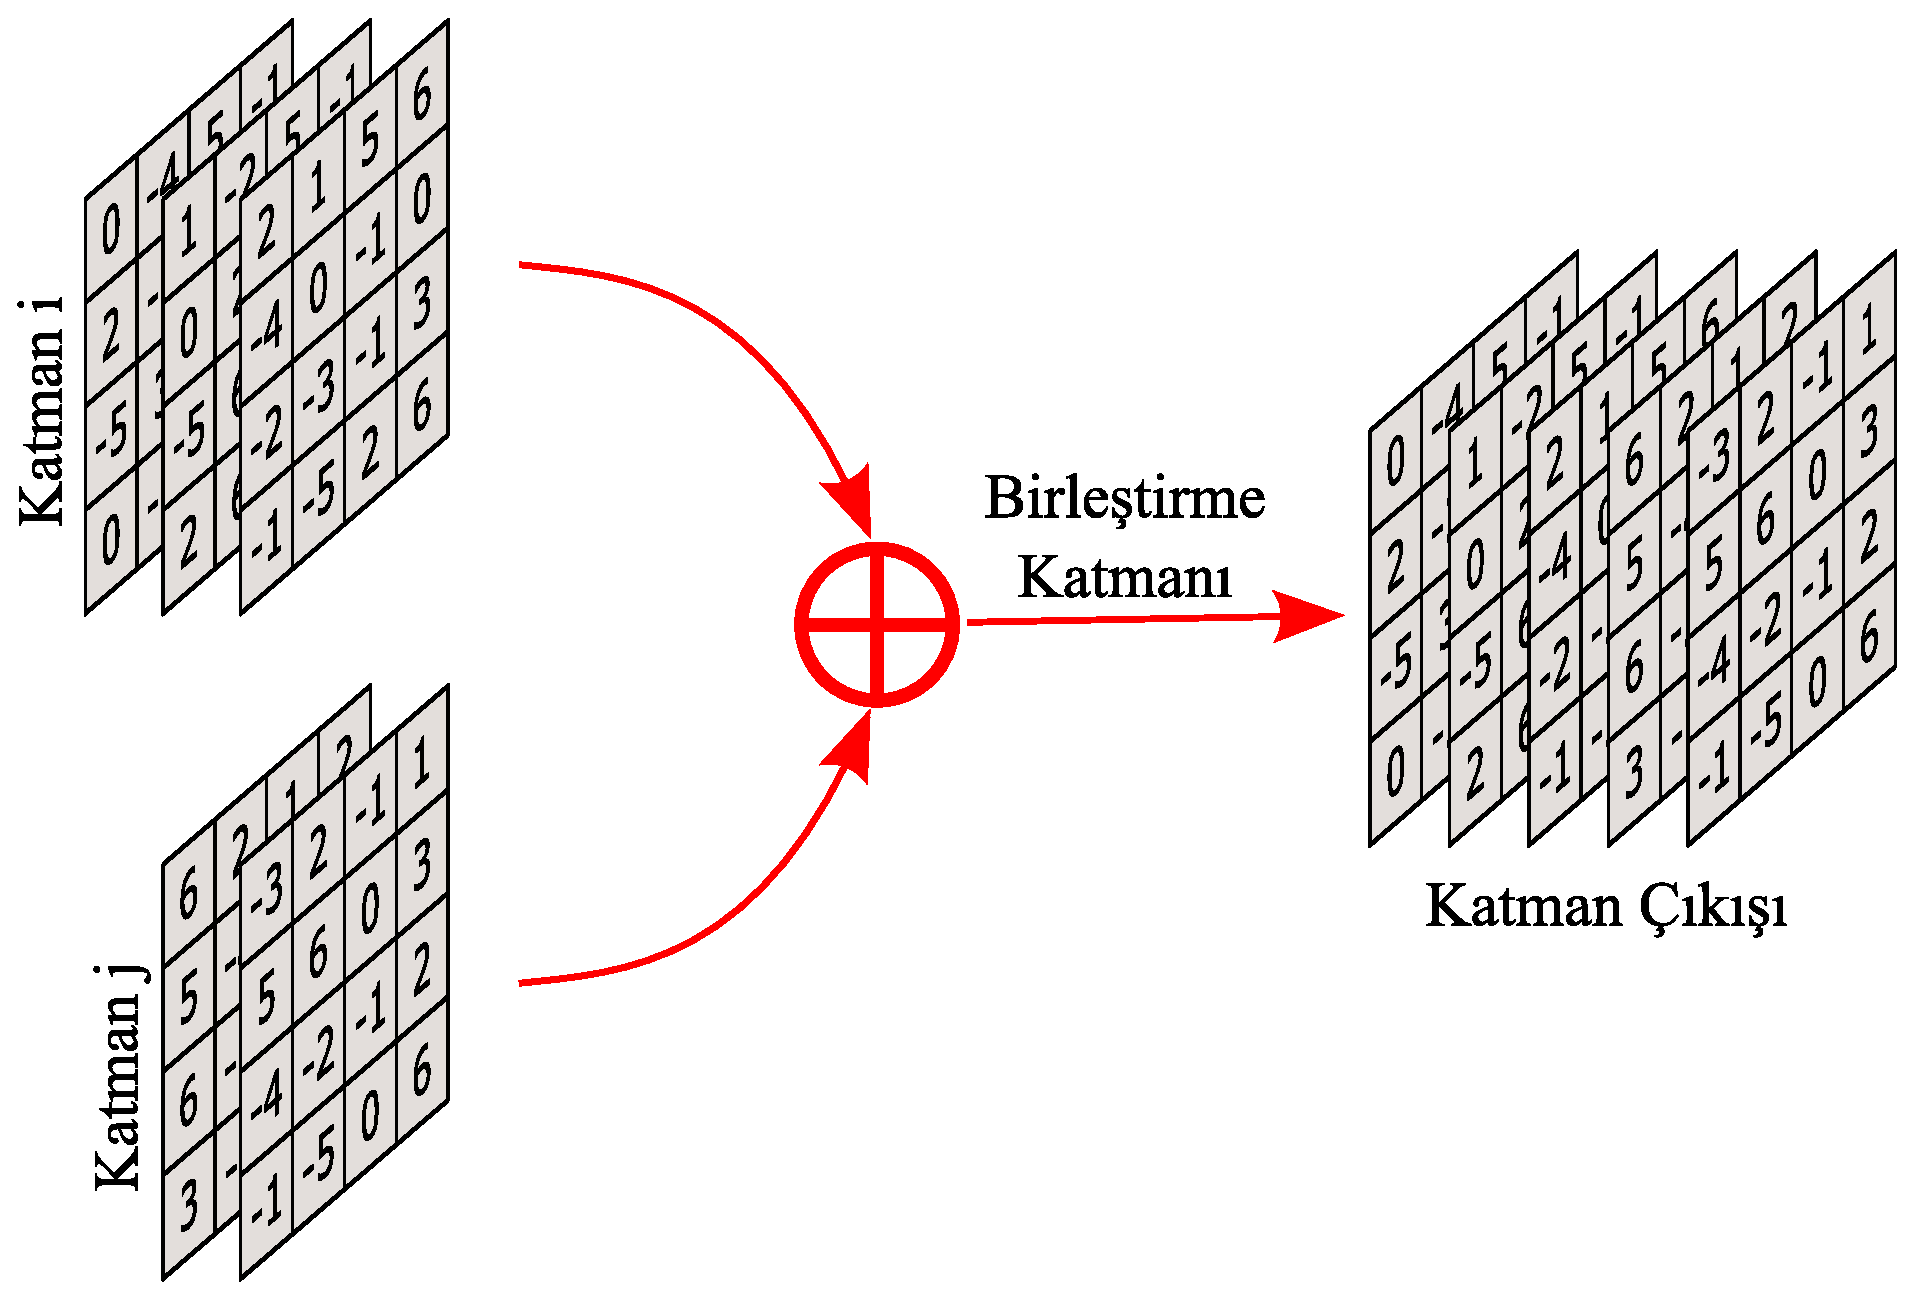
\includegraphics[scale=0.43]{Yapilan-Calismalar/Figures/concatenate.pdf}
		}
	\end{center}
\end{figure}

İki farklı katmanın özellik haritası sayılarının farklı olması durumunda derinlik birleştirme işlemi gerçekleştirilebilmektedir. Derinlik birleştirme katmanında iki farklı katman çıkışındaki özellik haritaları Şekil \ref{fig:concatenate}'de gösterildiği gibi birleştirilmektedir. Derinlik birleştirme katmanları genellikle oto-kodlayıcılarda karşımıza çıkmaktadır. Çok tercih edilen U-Net oto kodlayıcılarılarında \cite{ronneberger2015u} atlama bağlantıları ile konvolüsyon ve ters konvolüsyon katmanlarının çıktıları derinlik birleştirme işlemi ile birleştirilmektedir.

İki farklı katmanın özellik haritalarının aynı sayıda olması durumunda ise derinlik birleştirme işlemi gerçekleştirilebildiği gibi ekleme işlemi de gerçekleştirilebilmektedir. Ekleme katmanı iki katmandaki aynı indisli özellik haritalarını birleştirerek Şekil \ref{fig:add}'de gösterildiği gibi aynı sayıda özellik haritası üretmektedir. Özellik haritaları için ekleme işlemi literatürde ilk kez ResNet mimarisinde \cite{he2016deep} rastlanmaktadır. Derin ağlarda ilk katmanlardaki özellik haritalarında bulunan bilgiler katman sayısı arttıkça kaybolmaya başlamaktadır. Bu sebeple ekleme katmanı kullanılarak önceki katmanlardaki bilgi ileri katmanlarla birleştirilmekte ve böylece önemli bilgi kaybının önüne geçilebilmektedir.

\captionsetup[figure]{margin={0.3cm,-1cm}}
\begin{figure}[h!]
	\begin{center}
		\vspace{0.4cm}
		\captionbox{Derinlik ekleme işlemi (Add).\label{fig:add}}
		{
			\vspace{0.4cm}
			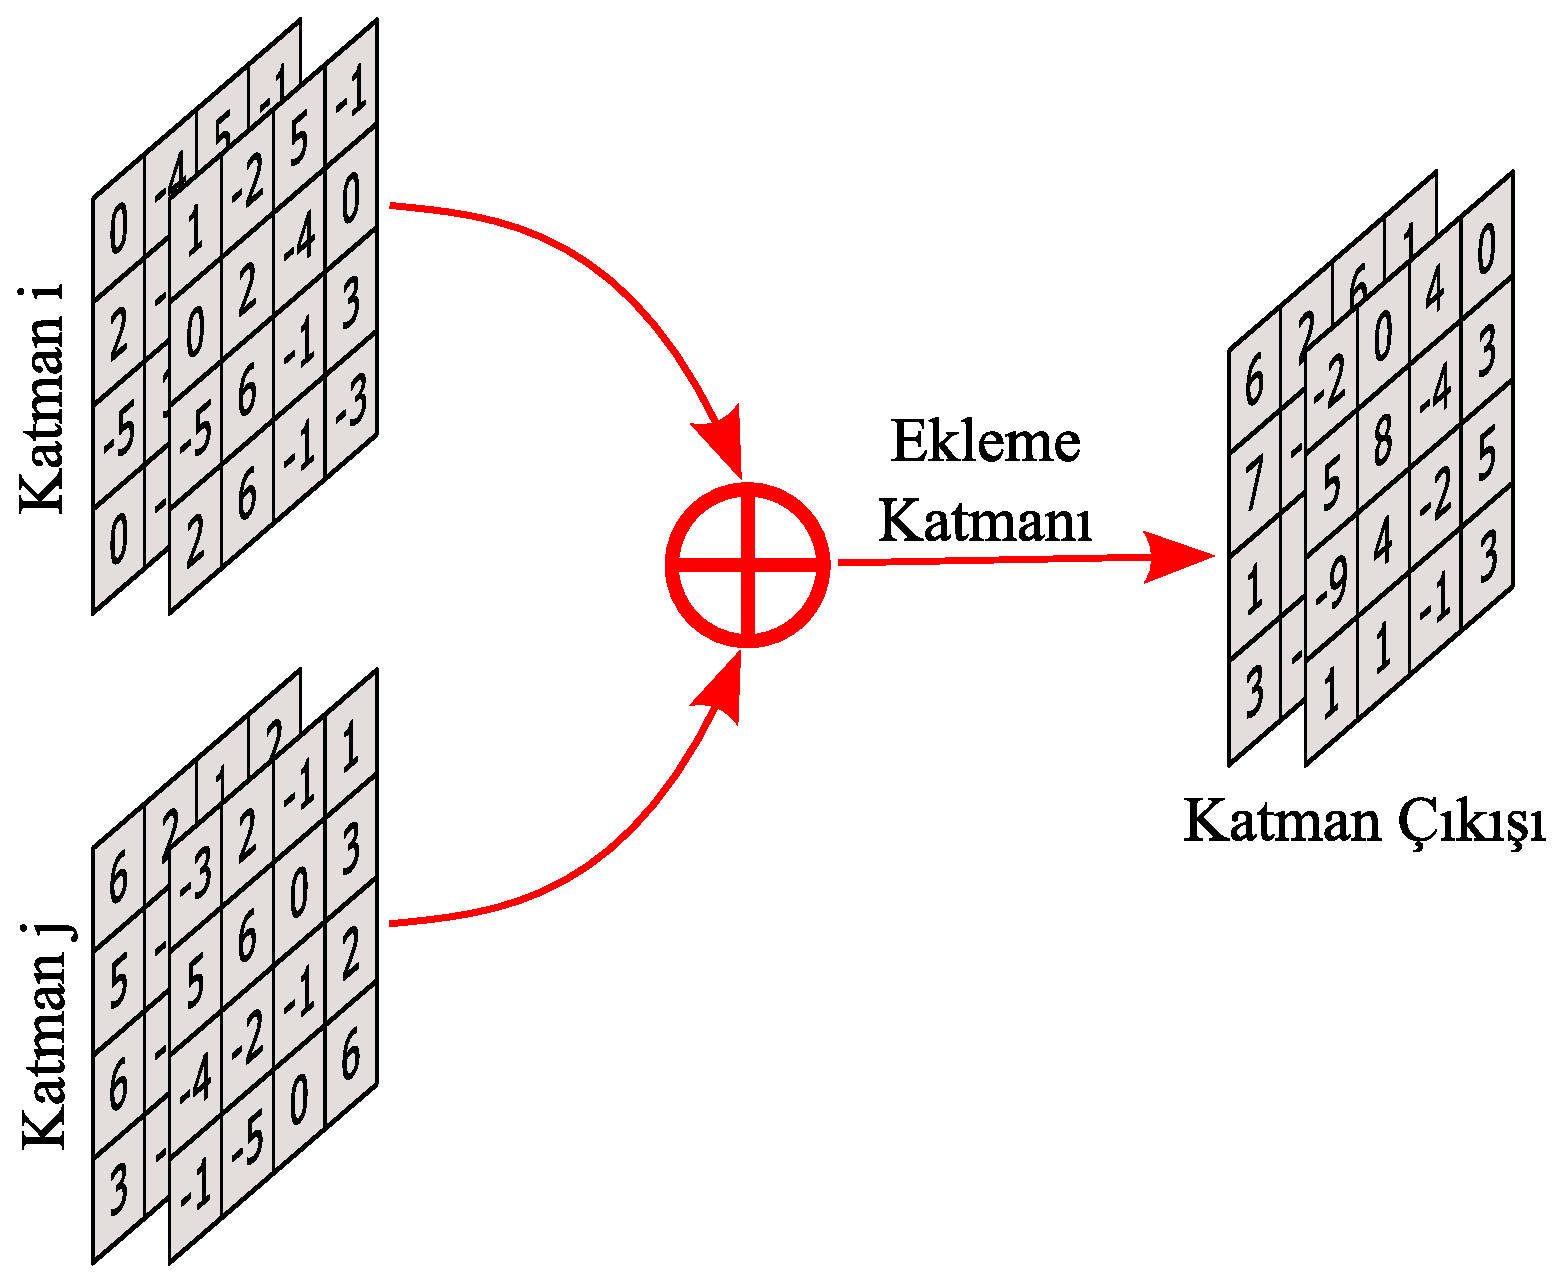
\includegraphics[scale=0.43]{Yapilan-Calismalar/Figures/add.pdf}
		}
	\end{center}
\end{figure}

\subsubsection{Düzleştirme Katmanları}
Düzleştirme (Flatten) katmanları girişinden $n$ boyutlu veri alıp çıkışından $n$ boyutlu veri üretebilen konvolüsyon gibi katmanların çıkışının sınıflandırma katmanlarına uydurulmasında kullanılan katmanlardır. Tam bağlantılı katmanlar giriş verisi olarak bir boyutlu $x$ vektörlerini kabul etmektedirler. Bu sebeple konvolüsyon katmanı gibi $n$ boyutlu çıkış üretebilen katmanların çıkışlarının sınıflandırıcı katmanlara aktarılmadan önce düzleştirilmesi gerekmektedir. Düzleştirme katmanlarının eğitilebilir parametresi bulunmamaktadır. Şekil \ref{fig:flattening}'te gösterildiği gibi düzleştirme katmanı girişinden uygulanan $n$ boyutlu veriyi bir boyutlu vektöre dönüştürmektedir. Düzleştirme katmanı girişinden birden çok özellik haritası uygulandığında birleştirme katmanlarında olduğu gibi verileri birleştirip bir boyutlu tek bir vektöre dönüştürmektedir.

\captionsetup[figure]{margin={0.3cm,-2cm}}
\begin{figure}[h!]
	\begin{center}
		\vspace{0.4cm}
		\captionbox{2B özellik haritasının düzleştirilmesi. \label{fig:flattening}}
		{
			\vspace{0.4cm}
			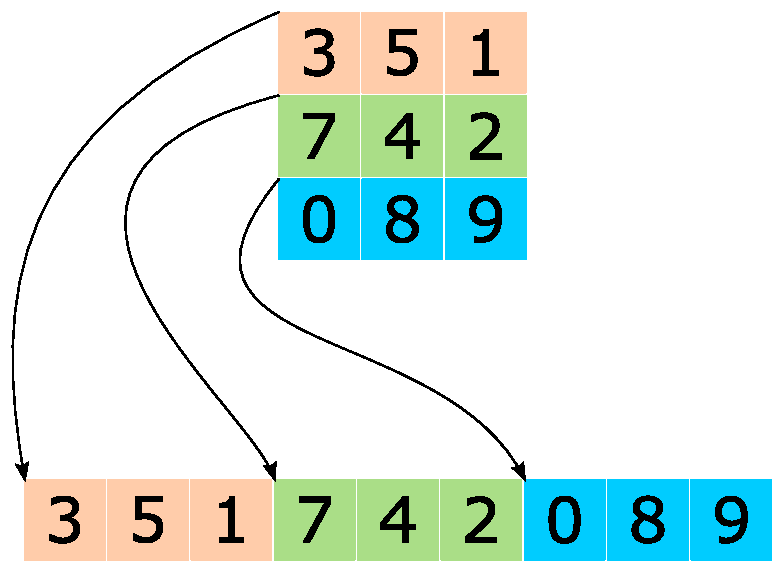
\includegraphics[scale=0.6]{Yapilan-Calismalar/Figures/flattening.pdf}
		}
	\end{center}
\end{figure}

\subsubsection{Seyreltme Katmanları \label{lyr:dropout}}
Seyreltme katmanları aslında bir düzenleştirme katmanıdır. Tam bağlantılı katmanlardan sonra kullanılarak ağın aşırı öğrenme (over fitting) problemi ile karşılaşmasını engelleme fikri ile ortaya atılmıştır \cite{srivastava2014dropout}. Kendisinden önce gelen tam bağlantılı katmandaki belirtilen oranda sinir hücresini rasgele olarak kapatarak eğitim aşamasında eğitim verisinin sürekli aynı yollar üzerinden akmasını engellemektedir. Bu katman sinir hücresi ağırlıklarının dengeli bir şekilde eğitilmesini sağlamaktadır. Rasgele sinir hücrelerinin kapatılmasındaki amaç tam bağlantılı katmanın herhangi bir sinir hücresine bağımlılığının azalmasıdır. Birlikte çalışan fazla sayıda sinir hücresi, modelin daha karmaşık işlevleri öğrenmesine de sebep verebildiği için seyreltme katmanlarının kullanılması modelin eğitim verilerindeki gürültü ve diğer bozulmalara daha dayanıklı olmasını sağlamaktadır.

Seyreltme katmanlarında kapatılan sinir hücreleri modelden çıkarılmış olmamaktadır. Sadece kapatılan sinir hücrelerinin çıkışları sıfırlanmaktadır. Bu sebeple modeldeki sinir hücresi sayısı değişmediğinden bu katmanın eğitim süresi üzerine hızlandırma etkisi bulunmamaktadır.

\captionsetup[figure]{margin={0.3cm,0cm}}
\begin{figure}[h!]
	\begin{center}
		\vspace{0.4cm}
		\captionbox{Tam bağlantılı katmana 0.5 oranında seyreltme gerçekleştiren seyreltme katmanı.\label{fig:dropout}}
		{
			\vspace{0.4cm}
			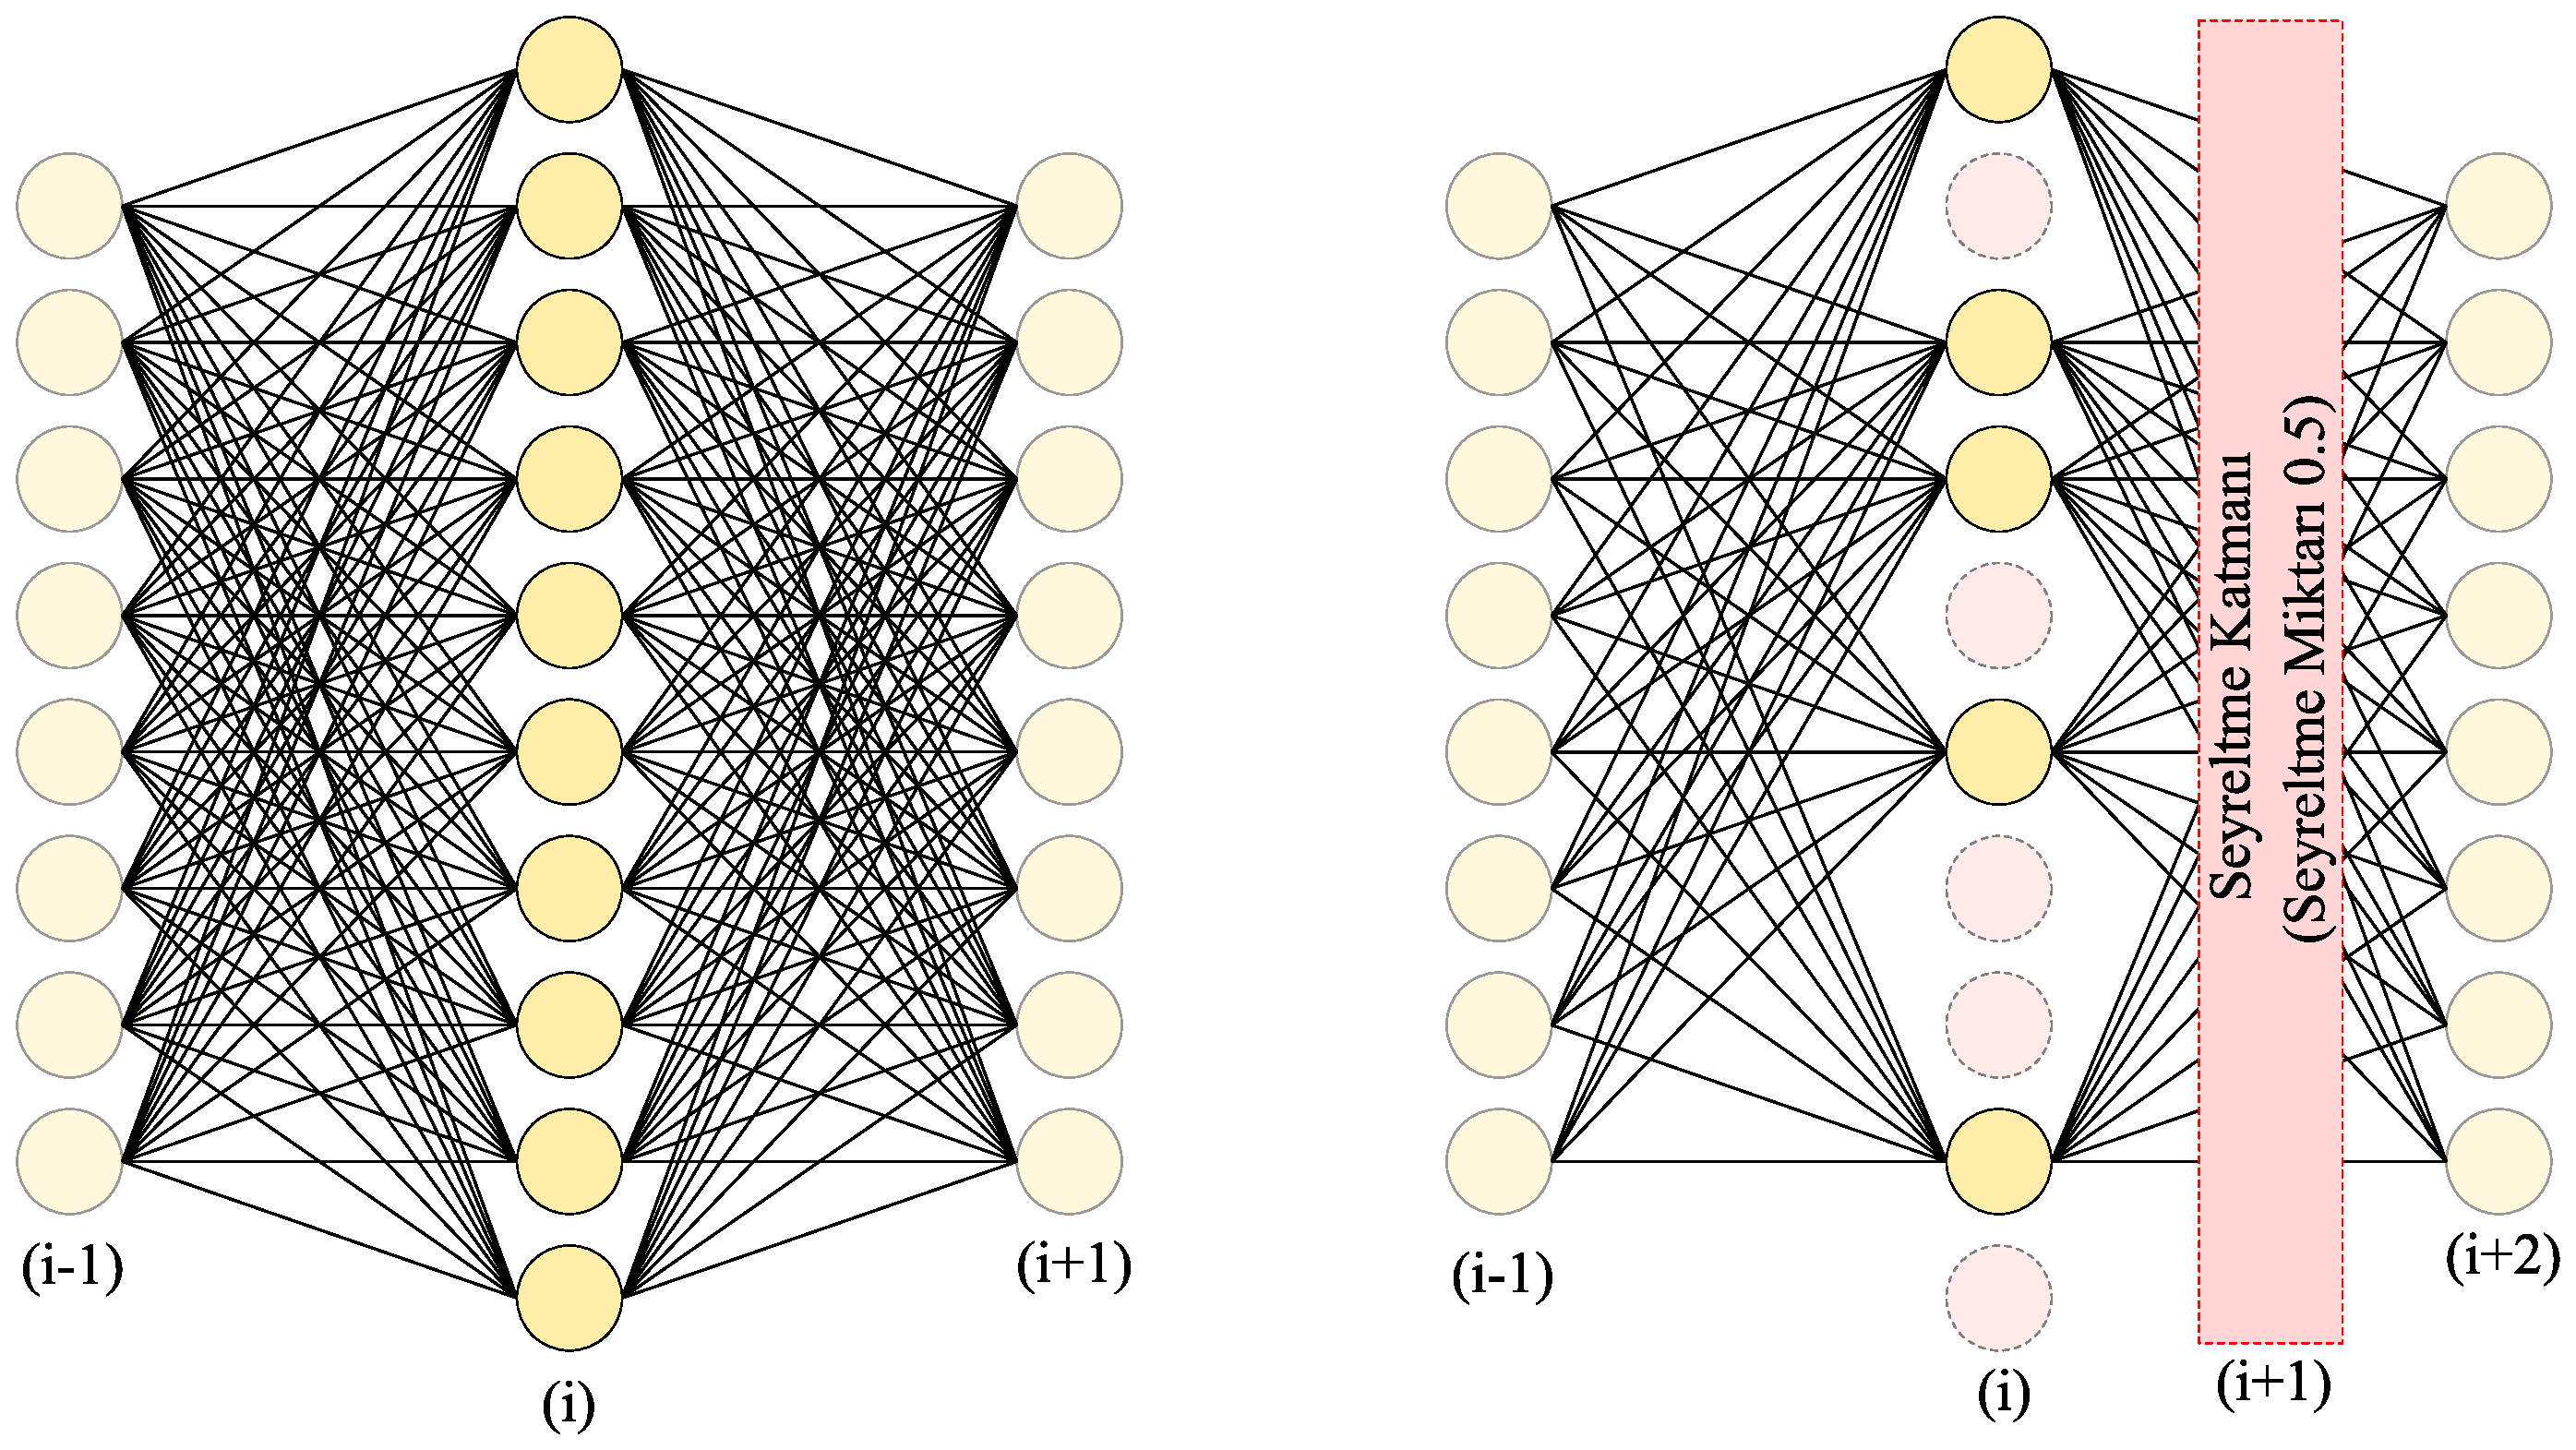
\includegraphics[scale=0.32]{Yapilan-Calismalar/Figures/dropout.pdf}
		}
	\end{center}
\end{figure}

Seyreltme katmanlarında rastgeleliği artırmak için genellikle Bernoulli dağılımı tercih edilmektedir. Bernoulli dağılımı, $p$ olasılığı ile $1$ değerinin ve $q$ olasılığı ile $0$ değerinin elde edilebildiği ikili (ayrık) bir olasılık dağılımıdır. Rasgele seçilmiş $r_{i}$ değerlerinden $r_{i}=1$ için Eşitlik \ref{eq:bernouli1}, $r_{i}=0$ için Eşitlik \ref{eq:bernouli0}'teki gibi bir olasılık söz konusu olmaktadır. Şekil \ref{fig:dropout}'te tam bağlantılı katmana 0.5 oranında seyreltme gerçekleştiren seyreltme katmanı gösterilmektedir.
\begin{equation}
	\label{eq:bernouli1}
	P(r_{i}=1) = p
\end{equation}
\vspace{-1cm}
\begin{equation}
	\label{eq:bernouli0}
	P(r_{i}=0) = q = 1 - p = 1 - P(r_{i}=1)
\end{equation}

Eşitlik \ref{eq:bernouli1} ve \ref{eq:bernouli0}'in anlamı, seyreltme değerinin $1$ olma olasılığının $p$ olduğu, $0$ olma olasılığı $q = 1 - p$ olduğudur. Böylece Eşitlik \ref{eq:bernouli2} elde edilmektedir.
\begin{equation}
	\label{eq:bernouli2}
	r_{i} \sim \textit{Bernoulli}(p)
\end{equation}

Eşitlik \ref{eq:bernouli2}'nın anlamı $r_{i}$ değerinin Bernoulli dağılımı $1$ olan bir $p$ olasılık değerinin eşdeğeri olduğudur. Bu olasılık dağılımları ile değeri $1$ olan $p$ dağılımına sahip sinir hücrelerinin çıkışları $1$ ile çarpılarak çalışmaya devam etmesi, değeri 0 olan sinir hücrelerinin çıkışları 0 ile çarpılarak seyreltilmesi sağlanmaktadır. $r_{i}$ inci sinir hücresinin çıkışını $z_{i}$ ve seyreltme katmanını $Sr$ olarak kabul edersek seyreltme işlemi Eşitlik \ref{eq:seyreltme}'deki gibi hesaplanmaktadır.
\begin{equation}
	\label{eq:seyreltme}
	Sr_{i} =  \left\{ 
	\begin{array}{ c l }
		\frac{z_{i}}{1-q} & \quad r_{i} = 1 \\
		0                 & \quad r_{i} = 0 
	\end{array}
	\right.
\end{equation}

Eğitim aşamasında her katmanda olduğu gibi seyreltme katmanının ters yönde hesaplaması gerçekleştirilirken zincir kuralına göre türevlenmesi gerekmektedir. Bu sebeple $r_{i}$ inci sinir hücresinin $z_{i}$ çıkışının $Sr$ seyreltme katmanına göre kısmi türevi Eşitlik \ref{eq:seyreltmederiv}'de verildiği gibi hesaplanmaktadır.
\begin{equation}
	\label{eq:seyreltmederiv}
	\frac{\partial}{\partial z_{i}}Sr_{i} =  \left\{ 
	\begin{array}{ c l }
		\frac{1}{1-q} & \quad r_{i} = 1 \\
		0                 & \quad r_{i} = 0 
	\end{array}
	\right. = \frac{r_{i}}{1-q}
\end{equation} 

\subsubsection{Paket Normalizasyon Katmanları \label{lyr:batchnormalization}}
Paket normalizasyon (Batch Normalization) katmanı aslında bir düzenleştirme katmanıdır. Bu katman derin ağların dahili ortak değişken kaymasını (Internal Covariate Shift) azaltarak eğitim hızlarını artırmayı hedeflemektedir \cite{ioffe2015batch}. Paket normalizasyon katmanları önüne eklendiği katman çıktılarını ortalamasını $0$'a ve varyansını $1$'e ölçeklendirmektedirler. Normalizasyon ya da özellik ölçeklendirmenin eğitim aşamasını hızlandırdığı prensibi paket normalizasyon katmanlarının ortaya çıkmasını sağlamıştır. Paket normalizasyon katmanları girişlerinden uygulanan $x$ verilerinin normalize $y$ verilerine dönüştürülmesini sağlayan fonksiyonun öğrenildiği katmanlardır.

Paket normalizasyon katmanında girişten uygulanan $m$ adet $x$ giriş verisinin ortalaması $\mu_{B}$ Eşitlik \ref{eq:bnmean}'da verildiği gibi hesaplanmaktadır. 
\begin{equation}
	\label{eq:bnmean}
	\mu_{B}=\frac{1}{m} \sum_{i=1}^{m} x_{i}
\end{equation}

Aynı $m$ adet $x$ giriş verisinin $\sigma^{2}_{B}$ varyansı Eşitlik \ref{eq:bnvariance}'daki gibi elde edilmektedir.
\begin{equation}
	\label{eq:bnvariance}
	\sigma_{B}^{2}=\frac{1}{m} \sum_{i=1}^{1}\left(x_{i}-\mu_{B}\right)^{2}
\end{equation}
Hesaplanan bu ortalama $\mu_{B}$ ve varyans $\sigma^{2}_{B}$ değerleri ile $x$ giriş setinin normalizasyonu Eşitlik \ref{eq:bnnormalize1}'deki gibi hesaplanmaktadır. Eşitlik \ref{eq:bnnormalize1}'de $\epsilon$ değeri varyans $\sigma^{2}_{B}$ değerinin $0$ olması durumunda $0$'a bölme hatası almamak için eklenen sıfıra çok yakın sabit değerdir.
\begin{equation}
	\label{eq:bnnormalize1}
	\hat{x}_{i}=\frac{x_{i}-\mu_{B}}{\sqrt{\sigma_{B}^{2}+\epsilon}}
\end{equation}
Normalizasyonu gerçekleştirilmiş $x$ giriş verisin bir eğitilebilir $\gamma$ standart sapma parametresi ile çarpılıp yine eğitilebilir bir $\beta$ ortalama parametresi eklenerek paket normalizasyon işlemi sonucu olan $y$ çıkışı Eşitlik \ref{eq:bnnormalize2} kullanılarak elde edilmektedir.
\begin{equation}
	\label{eq:bnnormalize2}
	y_{i}=\gamma \hat{x}_{i}+\beta
\end{equation}

Paket normalizasyon katmanları aktivasyon katmanlarından önce ya da sonra eklenebilmektedir. Fakat aktivasyon katmanlarından önce eklenmesi eğitime daha olumlu etki etmektedir.

\subsection{Kayıp Fonksiyonu ile Derin Ağın Hata Hesabı}
Kayıp fonksiyonu, oluşturulan bir öğrenme modelinin ürettiği çıkış $f(x)=\hat{ y }$ değeri ve eğitim setinde işaretli beklenen çıkış $y$ değeri arasındaki ilişkiyi temsil eden bir fonksiyondur. Öğrenme sürecinde eğitimde kullanılan temel bilgi kaynağı kayıp fonksiyonunun değeridir. Kayıp fonksiyonun değeri $[0,1]$ aralığında değişmektedir. Kayıp fonksiyonunun değeri $0$ değerine yaklaştıkça ağın ürettiği çıkış $\hat{ y }$ ve ağın beklenen çıkışı $y$ arasındaki fark azalmaktadır. Bu sebeple kayıp fonksiyonunun $0$ değerine yaklaşması hedeflenmektedir. 

Kayıp fonksiyonları regresyon işleminde kullanılan ve sınıflandırma işleminde kullanılan olmak üzere temelde ikiye ayrılmaktadırlar. Regresyon işlemi için tercih edilen kayıp fonksiyonlarına Ortalama Karesel Hata (Mean Square Error - MSE), Ortalama Mutlak Hata (Mean Absolute Error - MAE) ve Ortalama Önyargı Hatası (Mean Bias Error - MBE) örnek olarak verilebilmektedir. Sınıflandırmada tercih edilen kayıp fonksiyonları ise Menteşe Kayıp (Hinge Loss - HL), İkili Çapraz Entropi Kayıp (Binary Cross Entropy Loss - BCE) ve Kategorik Çapraz Entropi Kaybı (Categorical Cross Entropy Loss - CCE) olarak karşımıza çıkmaktadır. Ayrıca sınıf örnek sayılarının bir ya da daha fazla sınıfın lehine olacak şekilde dengesiz dağılımının söz konusu olduğu durumlarda Odak Kaybı  (Focal Loss - FL) kullanılabilmektedir \cite{lin2017focal}.  

Bu tez çalışmasında segmentasyon işlemi gerçekleştirilmektedir. Fakat aslında piksel düzeyinde düşünüldüğünde bir pikselin hangi sınıfa ait olduğu tespit edilmeye çalışılmaktadır. Dolayısıyla kayıp fonksiyonu olarak sınıflandırmada kullanılan kayıp fonksiyonlarından birinin kullanılması daha uygun olmaktadır. Bu çalışmada iki sınıflı segmentasyon için İkili Çapraz Entropi Kaybı ve çok sınıflı segmentasyon için ise Odak Kaybı fonksiyonları kullanmaktadır.  

\begin{itemize}
	\item Regresyonda Kullanılan Kayıp Fonksiyonları:
        \begin{itemize}
        	\item MSE Kayıp Fonksiyonu: 
        	
        	MSE kayıp fonksiyonunda $n$ adet çıkış algılayıcı sayısına sahip bir modelin $i$ inci algılayıcısının beklenen $y_{i}$ çıkışı için elde edilen $\hat{y}_{i}$ çıkışına göre hatası Eşitlik \ref{eq:mseloss}'te görüldüğü gibi hesaplanmaktadır.
        	{\setlength{\mathindent}{-1cm}
        	\begin{equation}
        		\label{eq:mseloss}
        		L_{MSE}=\frac{\sum_{i=1}^{n}\left(y_{i}-\hat{y}_{i}\right)^{2}}{n}
        	\end{equation}}
        	\item MAE Kayıp Fonksiyonu: 
        	
        	MAE kayıp fonksiyonunda $n$ adet çıkış algılayıcı sayısına sahip bir modelin $i$ inci algılayıcısının beklenen $y_{i}$ çıkışı için elde edilen $\hat{y}_{i}$ çıkışına göre hatası Eşitlik \ref{eq:maeloss}'te verildiği gibi hesaplanmaktadır.
        	{\setlength{\mathindent}{-1cm}
        	\begin{equation}
        		\label{eq:maeloss}
        		L_{MAE}=\frac{\sum_{i=1}^{n}\left|y_{i}-\hat{y}_{i}\right|}{n}
        	\end{equation}}
        	\item MBE Kayıp Fonksiyonu: 
        	
        	MBE kayıp fonksiyonunda $n$ adet çıkış algılayıcı sayısına sahip bir modelin $i$ inci algılayıcısının beklenen $y_{i}$ çıkışı için elde edilen $\hat{y}_{i}$ çıkışına göre hatası Eşitlik \ref{eq:mbeloss}'teki gibi hesaplanmaktadır.
        	{\setlength{\mathindent}{-1cm}
        	\begin{equation}
        		\label{eq:mbeloss}
        		L_{MBE}=\frac{\sum_{i=1}^{n}\left(y_{i}-\hat{y}_{i}\right)}{n}
        	\end{equation}}
        \end{itemize}

    \item  Sınıflandırmada Kullanılan Kayıp Fonksiyonları
    \begin{itemize}
    	\item HL Kayıp Fonksiyonu: 
    	
    	HL kayıp fonksiyonunda $n$ adet çıkış algılayıcı sayısına sahip bir modelin $i$ inci algılayıcısının beklenen $y_{i}$ çıkışı için elde edilen $\hat{y}_{i}$ çıkışına göre hatası Eşitlik \ref{eq:hlloss}'da verildiği gibi hesaplanmaktadır.
    	{\setlength{\mathindent}{-1cm}
    	\begin{equation}
    		\label{eq:hlloss}
    		L_{H}=\sum_{j \neq y_{i}} \max \left(0, s_{j}-s_{y_{i}}+1\right)
    	\end{equation}}
    	\item BCE Kayıp Fonksiyonu: 
    	
    	BCE kayıp fonksiyonu İki sınıflı sınıflandırmalarda tercih edilen ve çapraz entropi yöntemini kullanan bir kayıp fonksiyonudur. BCE kayıp fonksiyonunda $n$ adet çıkış algılayıcı sayısına sahip bir modelin $i$ inci algılayıcısının beklenen $y_{i}$ çıkışı için elde edilen $\hat{y}_{i}$ çıkışına göre hatası Eşitlik \ref{eq:bceloss}'de verildiği gibi hesaplanmaktadır.
    	{\setlength{\mathindent}{-1cm}
    	\begin{equation}
    		\label{eq:bceloss}
    		L_{BCE}=-\left(y_{i} \log \left(\hat{y}_{i}\right)+\left(1-y_{i}\right) \log \left(1-\hat{y}_{i}\right)\right)
    	\end{equation}}
    	\item CCE Kayıp Fonksiyonu: 
    	
    	CCE kayıp fonksiyonu çok sınıflı sınıflandırmada tercih edilen ve çapraz entropi yöntemini kullanan bir kayıp fonksiyonudur. CCE kayıp fonksiyonunda $n$ adet çıkış algılayıcı sayısına sahip bir modelin $i$ inci algılayıcısının beklenen $y_{i}$ çıkışı için elde edilen $\hat{y}_{i}$ çıkışına göre hatası Eşitlik \ref{eq:cceloss}'de gösterildiği gibi hesaplanmaktadır.
    	{\setlength{\mathindent}{-1cm}
    	\begin{equation}
    		\label{eq:cceloss}
    		L_{CCE_{i}}=-\sum_{j} y_{i, j} \log \left(\hat{y}_{i, j}\right)
    	\end{equation}}
    	\item FL Kayıp Fonksiyonu: 
    	
    	FL kayıp fonksiyonu çok sınıflı sınıflandırmada tercih edilen ve çapraz entropi yöntemini kullanan bir kayıp fonksiyonudur. Sınıfların örnek sayılarının herhangi bir sınıfın lehine olacak şekilde dengesiz dağıldığı durumlarda tercih edilmektedir. Sınıflar arası örnek sayılarının dengesiz olduğu durumlarda $\alpha$ ve $\gamma$ hiper parametreleri ile eğitimin dengelenmesi hedeflenmektedir.	
    	{\setlength{\mathindent}{-1cm}
    	\begin{equation}
    		\label{eq:flloss}
    		L_{FL(i)}=\left\{\begin{array}{cc}
                        -\alpha(1-\hat{y}_{i})^{\gamma} \log (\hat{y}_{i}), & y_{i}=1 \\
                        -(1-\alpha) \hat{y}_{i}^{\gamma} \log (1-\hat{y}_{i}), & \text { otherwise }
                        \end{array}\right.
    	\end{equation}}
    	$\alpha$ parametresinin $0$, $gamma$ parametresinin $1$ kabul edilmesi durumunda Çapraz Entropi kayıp fonksiyonu gibi davranmaktadır.
    \end{itemize}
\end{itemize}

\subsection{Geri Yayılım Algoritması}
Çok katmanlı mimarilerde eğitim, ileri yönlü hesaplama sonrasında elde edilen kayıp değeri kullanılarak gerçekleştirilmektedir. Dolayısıyla amaç kayıp fonksiyonu tarafından üretilen kayıp ($L$) değerini minimize etmektir. Kayıp fonksiyonunu minimize etmek için eğitilebilir katmanlardaki parametre değerlerinin değiştirilmesi gerekmektedir. Tam bağlantılı katmanlarda eğitilebilir parametreler ağırlık ve yanlılık ($w$ ve $b$) değerleri iken konvolüsyon ve ters konvolüsyon katmanlarında bu parametreler görüntü üzerinde gezdirilen filtre ($F$) değerleri olmaktadır.  

Geri yayılım algoritması her bir katmandaki eğitilebilir parametreleri güncelleyebilmek için kayıp fonksiyonunun ürettiği kayıp ($L$) değerinde gerçekleşen değişim bilgisini kullanmaktadır. Bu sebeple kayıp fonksiyonunun gradyanı hesaplanarak zincir kuralıyla çıkış katmanından giriş katmanına doğru $i$ inci katman $K_{i}$ olarak adlandırılmak üzere gradyan bilgisinin geri yayılımı Şekil \ref{fig:backpropagation}'teki gibi sağlanmaktadır. Geri yayılım algoritmasında her bir katmanın türevlerinin hesaplanması gerektiği için kayıp fonksiyonu, aktivasyon fonksiyonu gibi tüm işlemlerin türevleri kolay hesaplanabilir olması algoritmanın hesaplama yükünü oldukça azaltmaktadır.


\captionsetup[figure]{margin={0.5cm,-1cm}}
\begin{figure}[h!]
	\begin{center}
		\vspace{0.4cm}
		\captionbox{Geri Yayılım algoritmasında kayıp fonksiyonu ile hatanın geri yayılımı.\label{fig:backpropagation}}
		{
			\vspace{0.4cm}
			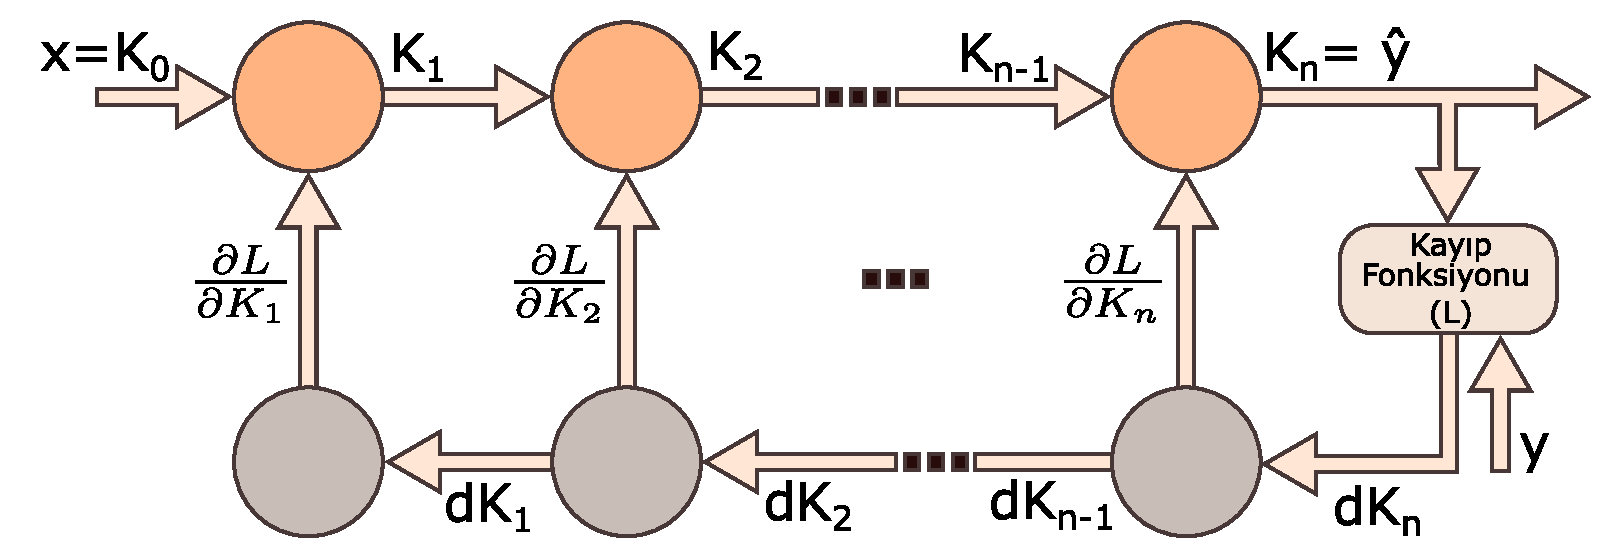
\includegraphics[scale=0.55]{Yapilan-Calismalar/Figures/backpropagation.pdf}
		}
	\end{center}
\end{figure}

Şekil \ref{fig:backpropagation}'te geri yayılım algoritmasında kısmi türevlerin hesaplanarak her katmandaki eğitilebilir parametrelerin güncellenebilmesi için zincir kuralı ile çıkış katmanından giriş katmanına doğru kısmı türev hesabının gerçekleştirilmesi gerektiği görülmektedir. Herhangi bir $m$ inci katmandaki eğitilebilir parametrelerin güncellenmesi için kullanılan kayıp fonksiyonundan elde edilen hataya göre kısmi türev hesabı Eşitlik \ref{eq:chain_rule}'de veridiği gibi hesaplanmaktadır.
\begin{equation}
	\label{eq:chain_rule}
	\frac{\partial L}{\partial  K_{m}} = \frac{\partial L}{\partial  K_{n}}\cdot\frac{\partial K_{n}}{\partial  K_{n-1}}\cdot...\cdot \frac{\partial K_{m+1}}{\partial  K_{m}}
\end{equation}

Her bir katmanda eğitilebilir katman parametrelerinin eğitimini gerçekleştirmek için hataya göre kısmi türevler hesaplanmakta ve hatanın minimize edilmesi için bu kısmi türev bilgisi kullanılmaktadır. Literatürde hatayı minimize edebilmek için kısmi türeve dayalı birçok optimizasyon tekniği mevcuttur. Bu optimizasyon tekniklerine bir sonraki bölümde değinilecektir.

\subsection{Geri Yayılım Algoritması Optimizasyon Teknikleri}
Geri yayılım algoritması kayıp fonksiyonu tarafından üretilen hatanın minimize edilmesini amaçlayan bir algoritmadır. Geri yayılım algoritmasında hatayı minimize etmek için eğitilebilir parametrelerin hataya göre kısmi türevini kullanan akıllı optimizasyon teknikleri derin ağın eğitim sürecini hızlandırabilmektedirler. 

Eğitilebilir tam bağlantılı katmanlardaki $W$, $b$ parametreleri ile konvolüsyon katmanlarındaki $F$ parametrelerinin herbiri için $\theta$ genel ifadesi kullanılmaktadır. Eğitilebilir $\theta$ parametresinin ağın toplam hatasına göre kısmi türevi Eşitlik \ref{eq:thetaderivative}'deki gibi ifade edilmektedir. İlgili $\theta$ parametresinde gerçekleştirilmesi gereken değişim kısmi hataya göre kısmi türev hesaplanılarak gerçekleştirilmektedir.
\begin{equation}
	\label{eq:thetaderivative}
	\frac{\partial}{\partial  \theta}L(\theta) = \nabla_{\theta}L
\end{equation} 

Kısmi türevin hatanın optimize edilmesindeki etkisi Şekil \ref{fig:gradyan}'da gösterilmektedir. Kısmi türev değerinin yönü hatanın minimize edilmesi için $\theta$ parametresinde gerçekleştirilmesi gereken negatif ya da pozitif yöndeki değişimin öngörülebilmesini sağlamaktadır.

\captionsetup[figure]{margin={0.5cm,-1cm}}
\begin{figure}[h!]
	\begin{center}
		\vspace{0.4cm}
		\captionbox{Gradyan bilgisinin hatanın minimize edilmesindeki etkisi.\label{fig:gradyan}}
		{
			\vspace{0.4cm}
			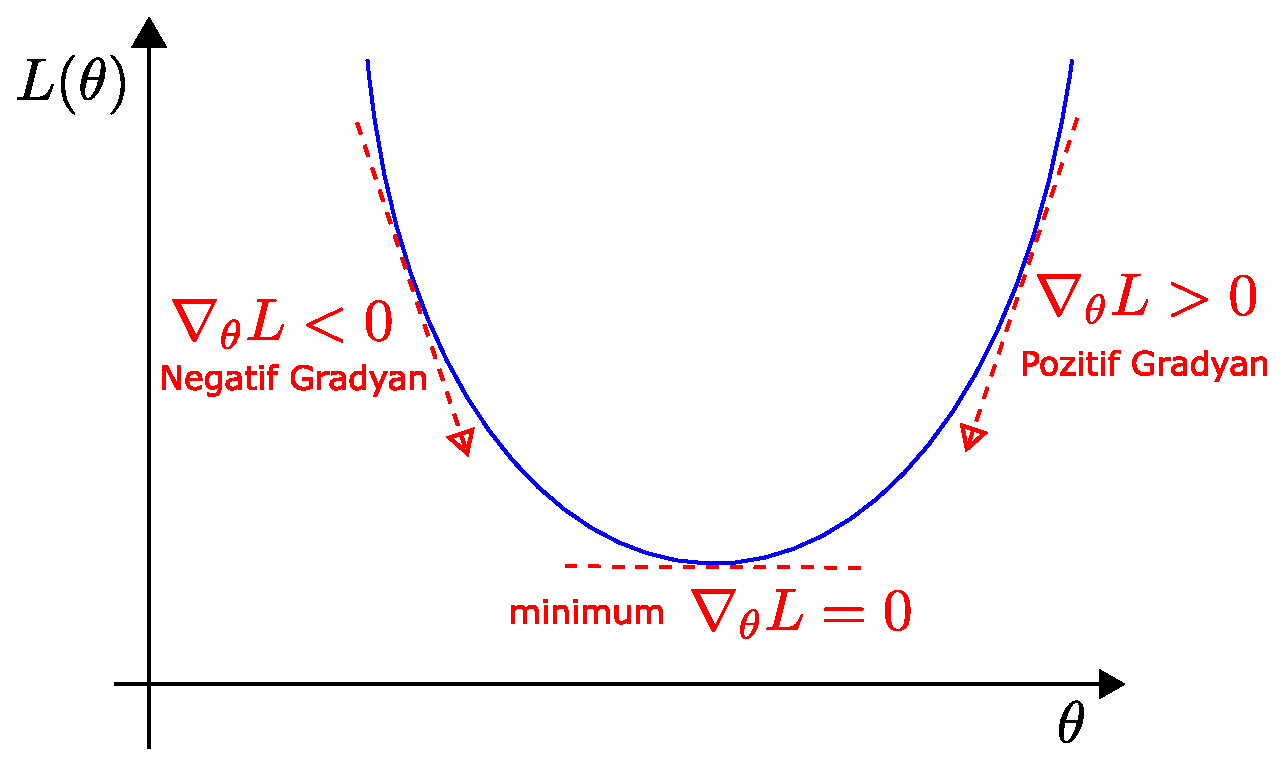
\includegraphics[scale=0.5]{Yapilan-Calismalar/Figures/gradyan.pdf}
		}
	\end{center}
\end{figure}

Çok katmanlı mimarilerde ağın eğitilmesi için genellikle bu gradyan bilgisinden faydalanan yöntemler tercih edilmektedir.

\subsubsection{Paket Gradyan Azalma}
Paket Gradyan Azalma (Batch Gradient Descent - BGD) yöntemi eğitimi tüm eğitim seti ile gerçekleştirmeyi öneren bir yaklaşımdır. BGD yöntemi hatayı minimize etmek için hesaplanan $\nabla_{\theta}L$ kısmi türevini bir $\alpha$ öğrenme katsayısı (learning rate) parametresi ile çarparak Eşitlik \ref{eq:batchgradiantdescent}'de görüldüğü gibi $\theta$ parametresine eklenilmesini önermektedir.
\begin{equation}
	\label{eq:batchgradiantdescent}
	\theta = \theta - \alpha \nabla_{\theta}L(\theta)
\end{equation} 

Öğrenme katsayısı bu yaklaşımda eğitimin başında bir kez atanmakta ve tüm eğitim boyunca aynı öğrenme katsayısıyla eğitim gerçekleştirilmektedir. Büyük veri kümelerinin eğitiminde tüm verinin eğitime tabi tutulmak zorunda olmasından dolayı hesaplama maliyeti oldukça yüksek bir yaklaşımdır.

\subsubsection{Mini-Paket Gradyan Azalma}
Mini-Paket Gradyan Azalma (Mini-Batch Gradient Descent) yöntemi Paket Gradyan Azalma yönteminin aksine tüm verinin değil paket boyutu (batch size) parametresine bağlı olarak verinin alt paketlere bölünerek eğitilmesini önermektedir. Bu sebeple bu yöntem eğitim her alt veri paketi için gerçekleştirilerek eğitim hesaplama maliyetinin düşürülmesi sağlanmaktadır. Tüm veri içinden $n$ adet alt veriyi seçerek Eşitlik \ref{eq:mbatchgradiantdescent}'te gösterildiği gibi hatanın optimize edilmesini hedeflemektedir.
\begin{equation}
	\label{eq:mbatchgradiantdescent}
	\theta = \theta - \alpha \nabla_{\theta}L(\theta;x^{(i:i+n)};y^{(i:i+n)})
\end{equation} 

Eğitimde tüm verinin kullanılmamasının sağladığı hız avantajının yanında eğitilebilir parametrelerin her küçük alt paket sonunda gerçekleştirdiği için eğitimin daha tutarlı olmasını sağlamaktadır.

\subsubsection{Stokastik Gradyan Azalma}
Stokastik Gradyan Azalma (Stochastic Gradient Descent - SGD) yöntemi tüm veri setiyle eğitimi gerçekleştirmek yerine her bir veri ile derin ağı tek tek eğitime tabi tutarak eğitilebilir parametrelerin güncellenmesini sağlamaktadır. Bu sebeple eğitim her örnek için ayrı ayrı gerçekleştirilmektedir. SGD yöntemi ile eğitilebilir parametrelerin eğitimi Eşitlik \ref{eq:sgradiantdescent}'te verildiği gibi gerçekleştirilmektedir.
\begin{equation}
	\label{eq:sgradiantdescent}
	\theta = \theta - \alpha \nabla_{\theta}L(\theta;x^{i};y^{i})
\end{equation} 
Her bir veri ile eğitim tek tek gerçekleştirildiği için hesaplama maliyeti oldukça yüksek bir yöntemdir.

\subsubsection{Momentumlu Stokastik Gradyan Azalma}
Momentumlu Stokastik Gradyan Azalma yöntemi temelinde hatanın gradyanının değişimindeki momentuma göre eğitim gerçekleştirmektedir. Optimizasyonun temel fizik kuramından destek alınarak gerçekleştirildiği bu yaklaşımda hatanın eğimi çok yüksek olduğunda fazla ivme kazandırılarak eğitimin lokal minimumlara takılmasının önüne geçilmektedir. Eğimdeki değişim azaldıkça ivme azaltılarak hatanın optimizasyonu sağlanmaktadır.

Momentumlu Stokastik Gradyan Azalma yöntemi standart SGD optimizasyon yöntemi modifiye edilerek geliştirilmiştir. Eğitilebilir $\theta$ parametrelerinin güncellenmesi Eşitlik \ref{eq:msgradiantdescent}'te görüldüğü gibi gerçekleştirilmektedir. Bu teknikte ivmenin kontrolü $\upsilon$ hız parametresi ile, hızın kontrolü ise $\mu$ sürtünme parametresi (momentum) ile gerçekleştirilerek global minimumu yakalamak hedeflenmektedir.
\begin{equation}
	\label{eq:msgradiantdescent}
	\begin{array}{ r l }
		\upsilon = &  \mu\upsilon - \alpha \nabla_{\theta}L(\theta) \\
		\theta = & \theta + \upsilon
	\end{array}
\end{equation}

Momentumlu Stokastik Gradyan Azalma yönteminde SGD yöntemine göre çok küçük bir değişiklik olmasına rağmen öğrenme hızında SGD yönteminden çok büyük bir artış söz konusudur.

\subsubsection{Adaptif Gradyan Algoritması}
Adaptif Gradyan Algoritması (Adaptive Gradient - AdaGrad) SGD algoritmasının her eğitilebilir parametreye özgü öğrenme katsayısı kullanma mantığı ile geliştirilmiş bir optimizasyon yöntemidir \cite{duchi2011adaptive}. Az karşılaşılan parametrelerin daha önemli bilgiler barındırabileceği mantığını savunan AdaGrad yönteminde öğrenme katsayısı $\alpha$ daha nadir rastlanan parametrelerde artırılırken daha sık rastlanan parametrelerde düşürülmektedir. 

AdaGrad algoritmasında eğitim sürecinde öğrenme katsayısı $\alpha$ kullanılmakta ve $\tau$ inci iterasyondaki hatanın kısmi türevi $g_{\tau}=\nabla L(\theta)$ olmak üzere, $\alpha$ öğrenme katsayısı değeri $G=\sum_{\tau=1}^{t} g_{\tau} g_{\tau}^{\mathrm{T}}$ dış çarpım matrisinin diyagonali olan $\left\{G_{j, j}\right\}$ vektörü ile çarpılmaktadır. $G_{j, j}=\sum_{\tau=1}^{t} g_{\tau, j}^{2}$ vektörü her iterasyonda güncellenmekte ve $\theta$ eğitilebilir parametrelerinin güncellenmesi Eşitlik \ref{eq:adagrad}'da verildiği gibi gerçekleştirilmektedir. Böylece her eğitilebilir $\theta_{i}$ parametresi için bir ölçekleme faktörü belirlenmiş olmaktadır. \begin{equation}
	\label{eq:adagrad}
	\theta_{j} = \theta_{j}-\frac{\alpha}{\sqrt{G_{j, j}}} g_{j}
\end{equation}

\subsubsection{Ortalama Karekök Yayılım Algoritması}
Ortalama Karekök Yayılım algoritması (Root Mean Square Propagation - RMSProp), sinir ağlarının eğitiminde kullanılan gradyan tabanlı optimizasyon tekniklerinden birisidir \cite{tieleman2012lecture}. RMSprop tekniği mini-paket öğrenme için geliştirilmiş bir stokastik tekniktir. RMSprop tekniği gradyanı normalleştirmek için kare gradyanların hareketli ortalamasını kullanarak kaybolan gradyan problemini ortadan kaldırmayı amaçlamaktadır. RMSprop tekniğindeki ana fikir, eğitilebilir bir parametre için öğrenme oranını, o ağırlık için son gradyanların büyüklüklerinin değişen bir ortalamasına bölmektir. Bu nedenle, unutma faktörü $\beta$ olarak temsil edilmek üzere öncelikle gradyanların ortalaması ortalama karekök cinsinden Eşitlik \ref{eq:rmsprop1}'deki gibi hesaplanmaktadır.
\begin{equation}
	\label{eq:rmsprop1}
	v(\theta, t)=\beta v(\theta, t-1)+(1-\beta)\left(\nabla L_{i}(\theta)\right)^{2}
\end{equation}
Daha sonra eğitilebilir parametreler bu değer ile Eşitlik \ref{eq:rmsprop2}'de görüldüğü gibi güncellenmektedir.
\begin{equation}
	\label{eq:rmsprop2}
	\theta=\theta-\frac{\alpha}{\sqrt{v(\theta, t)}} \nabla L_{i}(\theta)
\end{equation}

\subsubsection{Adaptif Moment Tahmini Algoritması}
RMSprop yönteminin geliştirilmiş bir versiyonu olan Adaptif Moment Tahmini algoritması (Adaptive Moment Estimation - Adam) düşük mertebeden momentlerin uyarlanabilir tahminlerine dayanmaktadır. Bu algoritma stokastik amaç fonksiyonlarının birinci mertebeden gradyan tabanlı bir optimizasyon tekniğidir \cite{kingma2014adam}. Adam, günümüzde en çok tercih edilen ve en son teknoloji optimizasyon algoritmalarından biridir. Bu tez çalışmasında da Adam optimizasyon yöntemi tercih edilmiştir. 

Bu optimizasyon algoritmasında hem gradyanların hem de gradyanların ikinci momentlerinin ortalamaları kullanılmaktadır. İkinci moment tarafından normalleştirilen ilk moment güncellemenin yönünü vermektedir. Eğitimde $t$ mevcut eğitim iterasyonu indeksi, $\theta^{(t)}$ eğitilebilir parametreler ve $L^{(t)}$ kayıp fonksiyonu olmak üzere, Adam algoritmasının eğitilebilir parametre güncellemesi Eşitlik \ref{eq:adam5}'te verildiği gibi hesaplanmaktadır.
\begin{equation}
	\label{eq:adam1}
	m_{\theta}^{(t+1)} \leftarrow \beta_{1} m_{\theta}^{(t)}+\left(1-\beta_{1}\right) \nabla_{\theta} L^{(t)}
\end{equation}
\vspace{-1cm}
\begin{equation}
	\label{eq:adam2}
	v_{\theta}^{(t+1)} \leftarrow \beta_{2} v_{\theta}^{(t)}+\left(1-\beta_{2}\right) (\nabla_{\theta} L^{(t)})^{2}
\end{equation}
\vspace{-1cm}
\begin{equation}
	\label{eq:adam3}
	\hat{m}_{\theta}=\frac{m_{\theta}^{(t+1)}}{1-\beta_{1}^{t}}
\end{equation}
\vspace{-1cm}
\begin{equation}
	\label{eq:adam4}
	\hat{v}_{\theta}=\frac{v_{\theta}^{(t+1)}}{1-\beta_{2}^{t}}
\end{equation}
\vspace{-1cm}
\begin{equation}
	\label{eq:adam5}
	\theta^{(t+1)} = \theta^{(t)}-\alpha \frac{\hat{m}_{\theta}}{\sqrt{\hat{v}_{\theta}}+\epsilon}
\end{equation}

Adam optimizasyon tekniği formülizasyonunda $\alpha$ öğrenme katsayısı, $\beta_{1}$, $\beta_{2}$ unutma faktörü parametreleridir. $\epsilon$ ifadesi sıfıra bölünme hatasına yakalanmamak için sıfıra çok yakın küçük bir değer seçilmelidir.

\subsection{Derin Ağlarda Düzenleştirme}
Derin ağlarda modelin eğitiminin yeterli yapılmadığı ya da giriş verilerinin eğitimi gerçekleştirmek istediğimiz veri setini tam ifade edemediği, eksik eğitim verilerinin kullanıldığı gibi durumlarda eksik uyum (underfitting) durumu ortaya çıkmaktadır. Aynı zamanda eğitimin gereğinden fazla sürdürüldüğü durumlarda da model eğitim setindeki her bir örneği eksiksiz öğrenmeye çalışmakta ve problemi eğitim seti için mükemmel öğrenmiş gibi görünse de test setinde büyük hatalar yapılmasına sebebiyet veren aşırı öğrenme (overfitting) durumu ile karşılaşılmaktadır. Eğitimde amaç eğitim seti eğitiminin genelleştirilerek doğru öğrenmenin sağlanmasıdır. Eksik uyum, doğru uyum ve aşırı uyum durumları Şekil \ref{fig:regularization}'de gösterilmektedir.
\captionsetup[figure]{margin={0.5cm,-1cm}}
\begin{figure}[h!]
	\begin{center}
		\vspace{0.4cm}
		\captionbox{Modelin eksik öğrenmesi, doğru öğrenmesi ve aşırı öğrenmesi durumları.\label{fig:regularization}}
		{
			\vspace{0.4cm}
			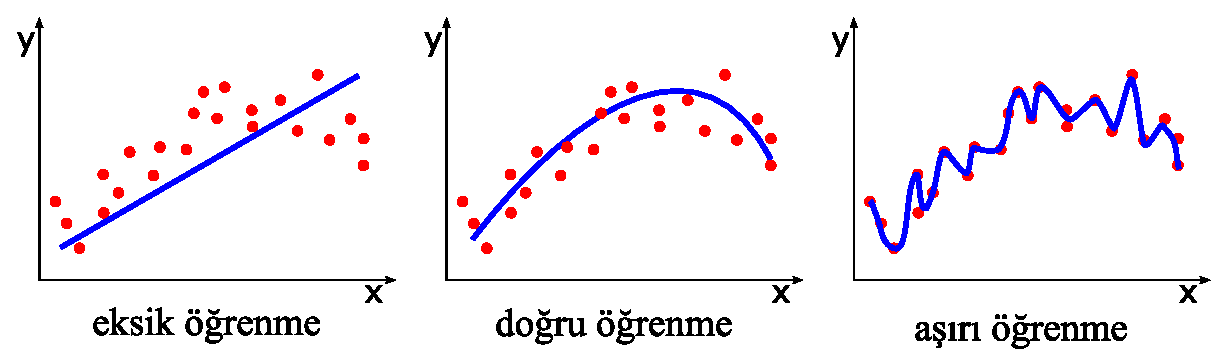
\includegraphics[scale=0.65]{Yapilan-Calismalar/Figures/regularization.pdf}
		}
	\end{center}
\end{figure}

Derin öğrenmede uyum problemlerini ortadan kaldırmak için literatürde birçok yöntem önerilmiştir \cite{girosi1995regularization}. Düzenleştirme işlemini gerçekleştiren katmanlardan olan Seyreltme katmanları ve Paket Normalizasyon katmanları sırasıyla Bölüm \ref{lyr:dropout} ve \ref{lyr:batchnormalization}'da incelenmiştir. Bu yöntemler haricinde literatürde Veri Artırma \cite{shorten2019survey}, L1 ve L2 Düzenleştirme \cite{ng2004feature} işlemleri de kullanılmaktadır.

\subsubsection{Veri Artırma} 
Derin ağlarda giriş verisi üzerinde gerçekleştirilen düzenleme yöntemlerinden birisidir. Derin öğrenmede eğitim verisi üzerinden iyi bir genelleştirme yapabilmek için çok sayıda görüntüye ihtiyaç duyulmaktadır. Veri artırma az sayıdaki giriş veri setini bazı transformasyon işlerine tabi tutarak artırmayı öneren bir yaklaşımdır. Veri artırmada öteleme, yansıtma, döndürme, ölçekleme, gürültü ekleme, kırpma gibi oldukça zengin transformasyon işlemleri kullanılabilmektedir. Şekil \ref{fig:augmentation}'de veri artırma tekniği ile farklı transformasyonlarda eğitim verisinin çoğaltılması gösterilmektedir. Derin ağlarda özellik çıkarma işlemi otomatikleştirildiği için çok sayıda görüntü ile genelleştirme yapmak çok daha güçlü özellik haritaları elde etmemizi sağlamaktadır. 

Veri artırmayı uygularken verinin transformasyon sonrası farklı bir sınıfa benzememesine dikkat etmek gerekmektedir. Örneğin el yazısı rakam sınıflandırmada veri artırma gerçekleştirirken döndürme transformasyonu 6 ve 9 rakamların birbiri ile karışmasına sebep olmaktadır. Ayrıca BT verisi gibi 2B dilimlerden oluşan 3B veri setlerinde kullanılan transformasyon tüm alt dilimler için aynı şekilde uygulanmalıdır. Segmentasyon problemlerinde de yine transformasyon hem giriş verisine hemde eğitim maske verilerine aynı şekilde uygulanmalıdır.

\captionsetup[figure]{margin={0.3cm,-0.5cm}}
\begin{figure}[h!]
	\begin{center}
		\vspace{0.4cm}
		\captionbox{Veri artırma tekniği ile farklı transformasyonlarda eğitim verisinin çoğaltılması.\label{fig:augmentation}}
		{
			\vspace{0.4cm}
			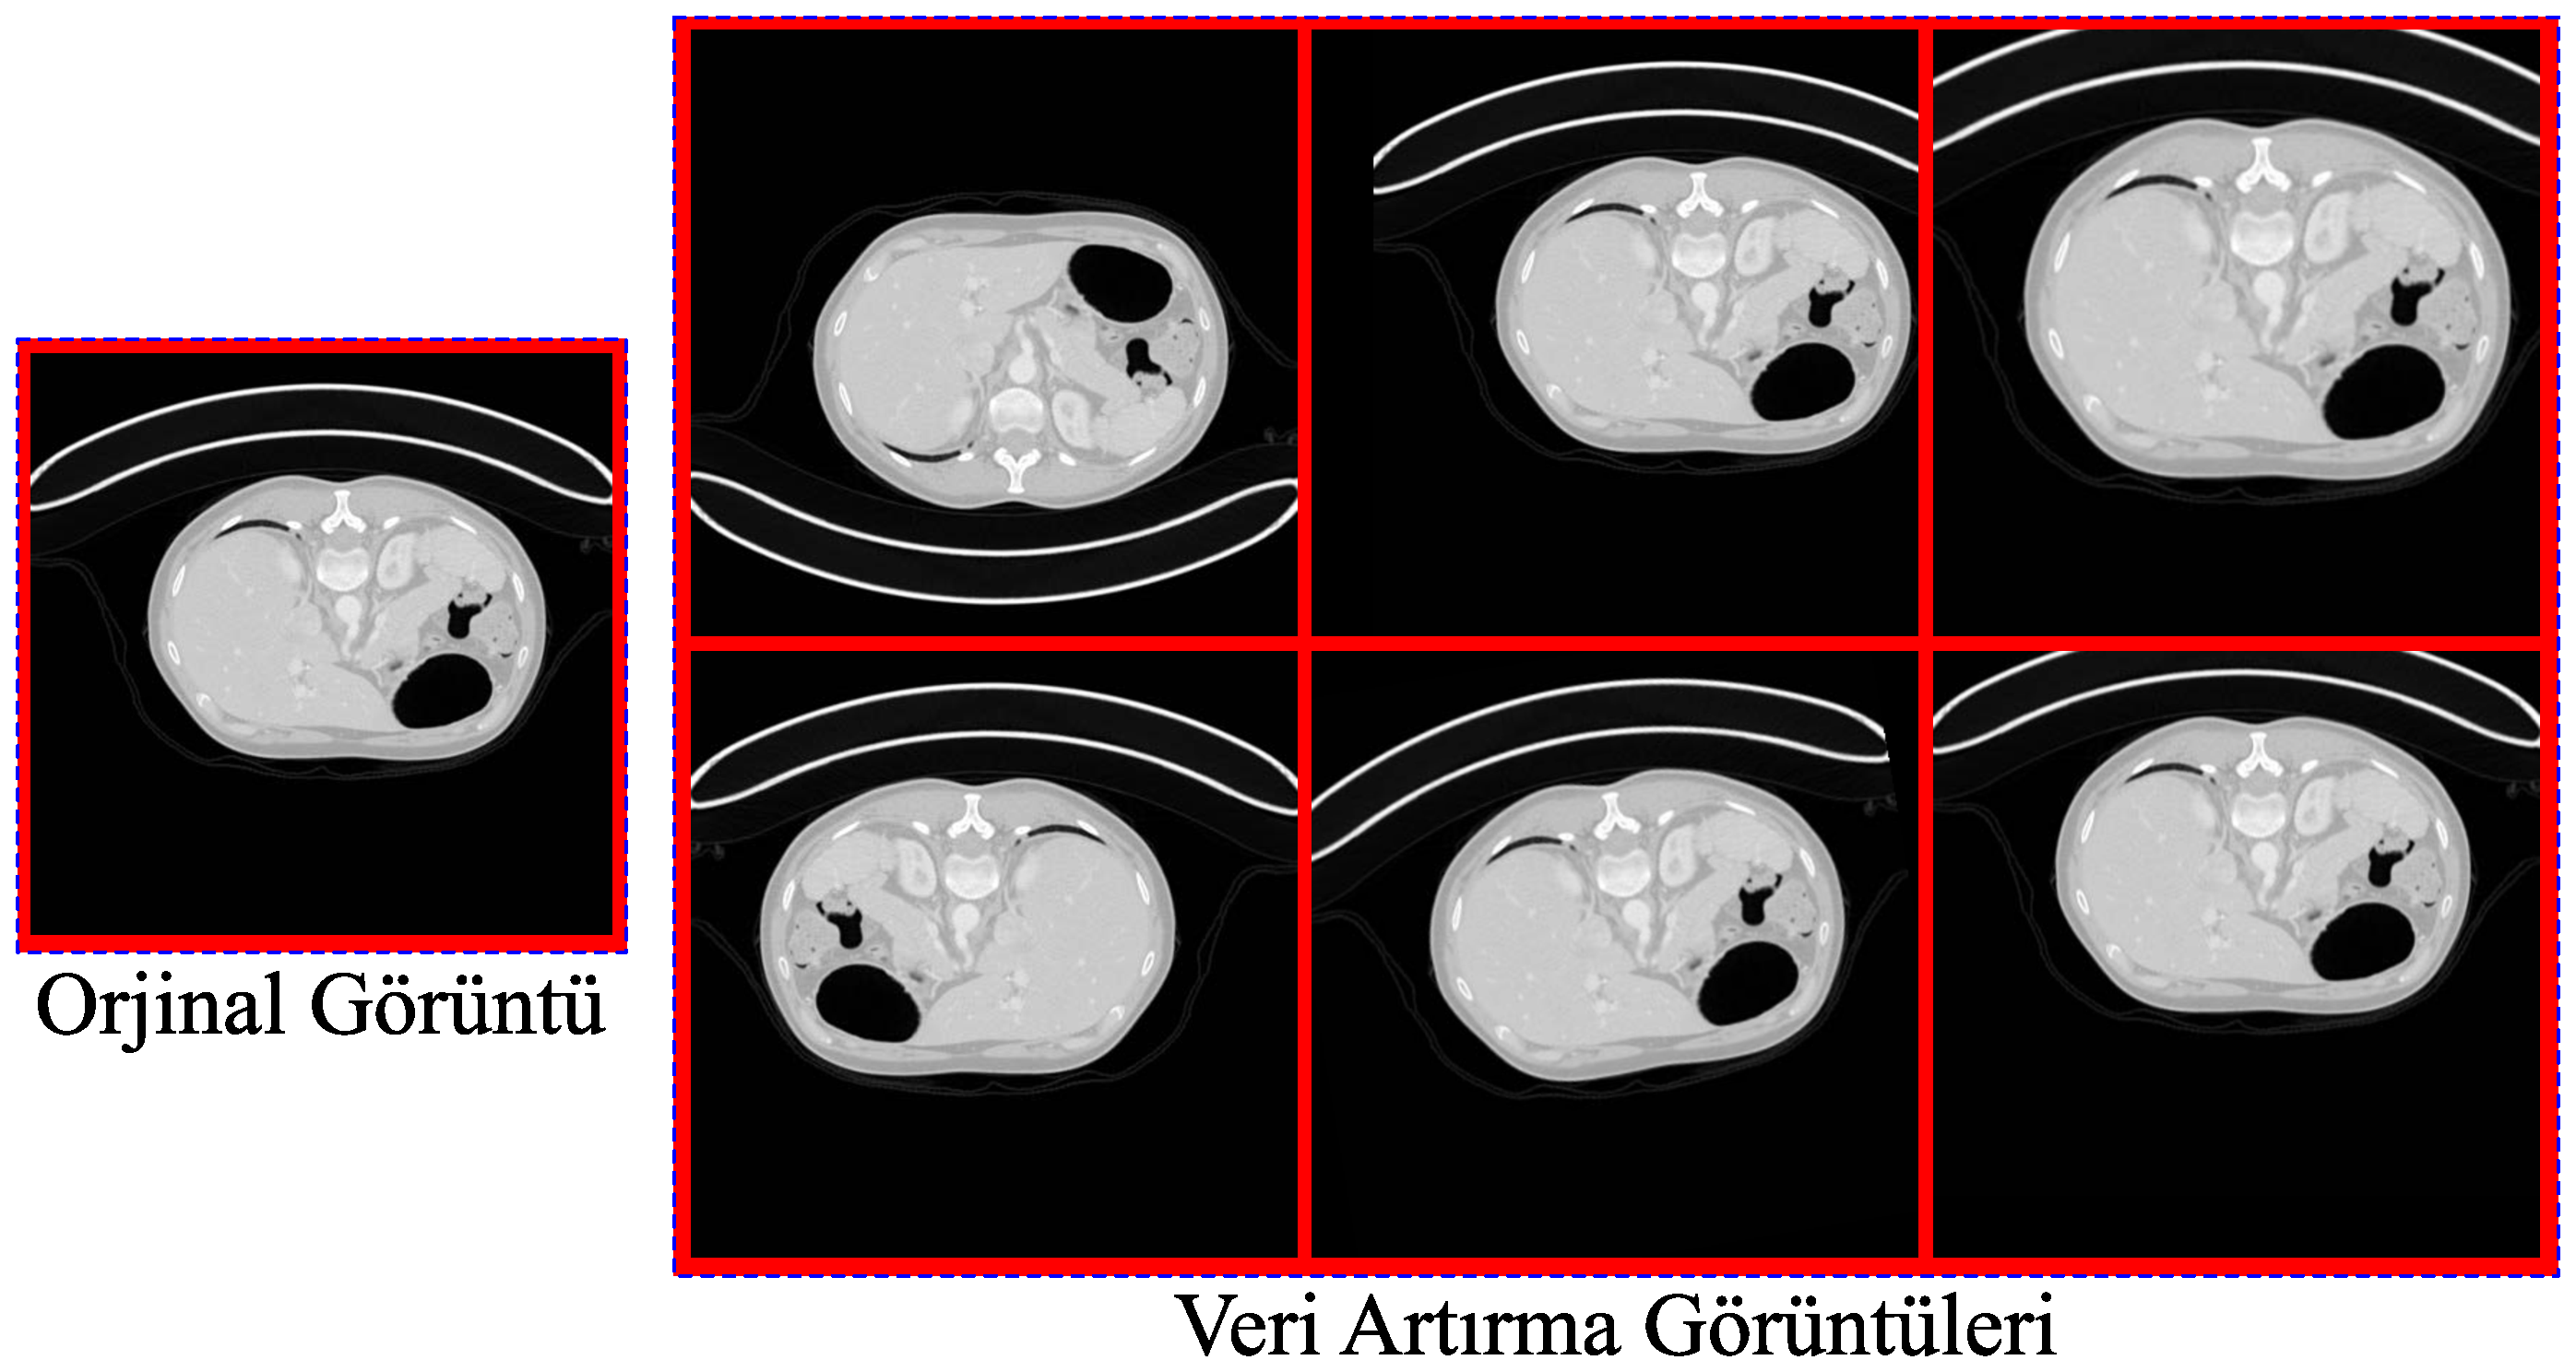
\includegraphics[scale=0.3]{Yapilan-Calismalar/Figures/augmentation.pdf}
		}
	\end{center}
\end{figure}

\subsubsection{L1 ve L2 Düzenleştirme} 
L1 ve L2 düzenleştirmeler aşırı öğrenmenin önüne geçebilmek için tam bağlantılı katmanlardaki eğitilebilir ağırlık $w$ ve yanlılık $b$ parametrelerini $\theta$ genel adıyla tanımlamak üzere sırasıyla Eşitlik \ref{eq:l1reg} ve \ref{eq:l2reg}'te verildiği gibi hesaplanmaktadır.
\begin{equation}
	\label{eq:l1reg}
	L_{1 \theta}=\lambda \sum_{m}\left|\theta_{m}\right|
\end{equation}
\vspace{-1cm}
\begin{equation}
	\label{eq:l2reg}
	L_{2 \theta}=\lambda \sum_{m}\theta_{m}^{2}
\end{equation}
Tam bağlantılı katmandaki eğitilebilir parametreler için tanımlanan cezalandırma katsayısı $\lambda$ ağırlık $w$ ve yanlılık $b$ değerleri için ayrı ayrı tanımlanarak $L_{1w}$, $L_{2w}$, $L_{1b}$ ve $L_{2b}$ değerleri hesaplanabilmektedir. Hesaplanan bu L1 ve L2 cezalar ağın genel hatasına Eşitlik \ref{eq:l1l2reg}'daki gibi eklenerek eğitim gerçekleştirilmektedir. Böylece ağın genel hata değeri ($L$) L1 ve L2 düzenleştirme değerleri ile cezalandırılmaktadır. 
\begin{equation}
	\label{eq:l1l2reg}
	L = L + L_{1w} + L_{2w} + L_{1b} + L_{2b}
\end{equation}

%%%%%%%%%%%%%%%Önerilen Yöntem%%%%%%%%%%%%%%%%%%%%%%
\section{Pankreas İlgi Bölgesinin Belirlenmesi ve İlgi Bölgesinde Pankreas Segmentasyonu \label{sec:pancreas}}

Bu tez çalışmasında BT görüntülerinde bulunan, abdominal bölgede oldukça küçük bir alan kaplayan pankreas organının daha başarılı segmentasyonu hedeflenmektedir. Bu hedef için tez çalışmasında kabadan inceye yöntemi ile pankreas ilgi bölgesinin belirlenmesi ve bu ilgi bölgesinde pankreas segmentasyonunun gerçekleştirilmesine yönelik bir yaklaşım önerilmektedir. Bu yaklaşım Pankreas İlgi Bölgesinin   Belirlenmesi ve İlgi Bölgesinde Pankreas Segmentasyonu olmak üzere Şekil \ref{fig:proposed_aproach}'da gösterildiği gibi iki fazdan oluşmaktadır.

\captionsetup[figure]{margin={0.3cm,-0.3cm}}
\begin{figure}[h!]
	\begin{center}
		\vspace{0.4cm}
		\captionbox{ Pankreas Segmentasyonu için önerilen 2 fazlı (Pankreas İlgi Bölgesinin Belirlenmesi, Belirlenen İlgi Bölgesinde Pankreas Segmentasyonu) yöntemin blok diyagramı.\label{fig:proposed_aproach}}
		{
			\vspace{0.4cm}
			\includegraphics[scale=0.695]{Yapilan-Calismalar/Figures/proposed_aproach.pdf}
		}
	\end{center}
\end{figure}

Yaklaşımın birinci fazında kaba pankreas bölgesinin tespiti için 2B segmentasyon yöntemlerinden olmasına karşın oldukça başarılı segmentasyon sonuçları üretebilen Mask R-CNN yöntemi tercih edilmektedir. Hasta bireylerin abdominal bölgelerinden çekilen ham 3B volümetrik BT verilerinin her bir 2B alt dilimi daha önce eğitim veri seti ile eğitilmiş Mask R-CNN modeline ayrı ayrı verilerek 2B segmentasyon gerçekleştirilmektedir. Segmentasyonu gerçekleştirilen her bir BT diliminin birleştirilmesi ile elde edilen 3B volümetrik veriden pankreas organının ilgi bölgesi kaba hatları ile belirlenmektedir. Kaba pankreas bölgesinde 2B bir yöntem tercih edilerek hesaplama yükünün düşürülmesi sağlanmaktadır.

Yaklaşımın ikinci fazında belirlenen ilgi bölgesi üzerinde 3B U-Net yöntemi ile tekrar segmentasyon gerçekleştirilerek pankreas organının daha hassas segmentasyonu gerçekleştirilmektedir. Hassas segmentasyon aşamasında bölgenin küçülmesinden kaynaklı hesaplama yükünün azalması ile 3B yöntemlerin kullanılabilir olması sağlanmaktadır. Böylece dilimler arasındaki süreklilik bilgisi dikkate alınarak daha hassas segmentasyon işlemi gerçekleştirilebilmektedir.

\subsection{Pankreas İlgi Bölgesinin Belirlenmesi}
Önerilen otomatik pankreas segmentasyon yaklaşımının ilk fazı olan Pankreas İlgi Bölgesinin Belirlenmesi, ($512 \times 512 \times N$) boyutundaki 2B BT dilimlerini giriş olarak almaktadır. Burada $N$, BT taramasındaki dilim sayısını temsil etmektedir. 2B alt BT dilimlerini ($256 \times 256 \times 2N / 3$) çıkış olarak üretmektedir. Pankreas İlgi Bölgesinin Belirlenmesi fazı, pankreas segmentasyonu için işlenen BT dilimlerinin boyutunu azaltmayı amaçlamaktadır. Bu faz Mask R-CNN ile Pankreas İlgi Bölgesinin Belirlenmesi ve Mask R-CNN'den elde edilen bilgi ile Kaba Pankreas Bölgesinin Belirlenmesi olmak üzere iki ana aşamadan oluşmaktadır.
 
\subsubsection{Mask R-CNN Modeli ile İlgi Bölgesinin Belirlenmesi}
Pankreas İlgi Bölgesinin Belirlenmesi aşamasında 2B BT dilimlerindeki ($512 \times 512 \times N$) kaba pankreas bölgelerinin tespit edilmesine odaklanılmıştır. Bu aşamada, Mask R-CNN yöntemi kullanılarak, 2B BT dilimlerinden hem sınırlayıcı kutuları elde edilmekte hem de kaba pankreas bölgelerinin bölümlere ayrılmış alt görüntüleri segmente edilmektedir.

\captionsetup[figure]{margin={0.4cm,-0.5cm}}
\begin{figure}[h!]
	\begin{center}
		\vspace{0.4cm}
		\captionbox{Pankreas İlgi Bölgesinin Belirlenmesi fazının Mask R-CNN modeli kullanan ilk aşamasındaki beş ana adımın şematik gösterimi.\label{fig:maskrcnn}}
		{
			\vspace{0.4cm}
			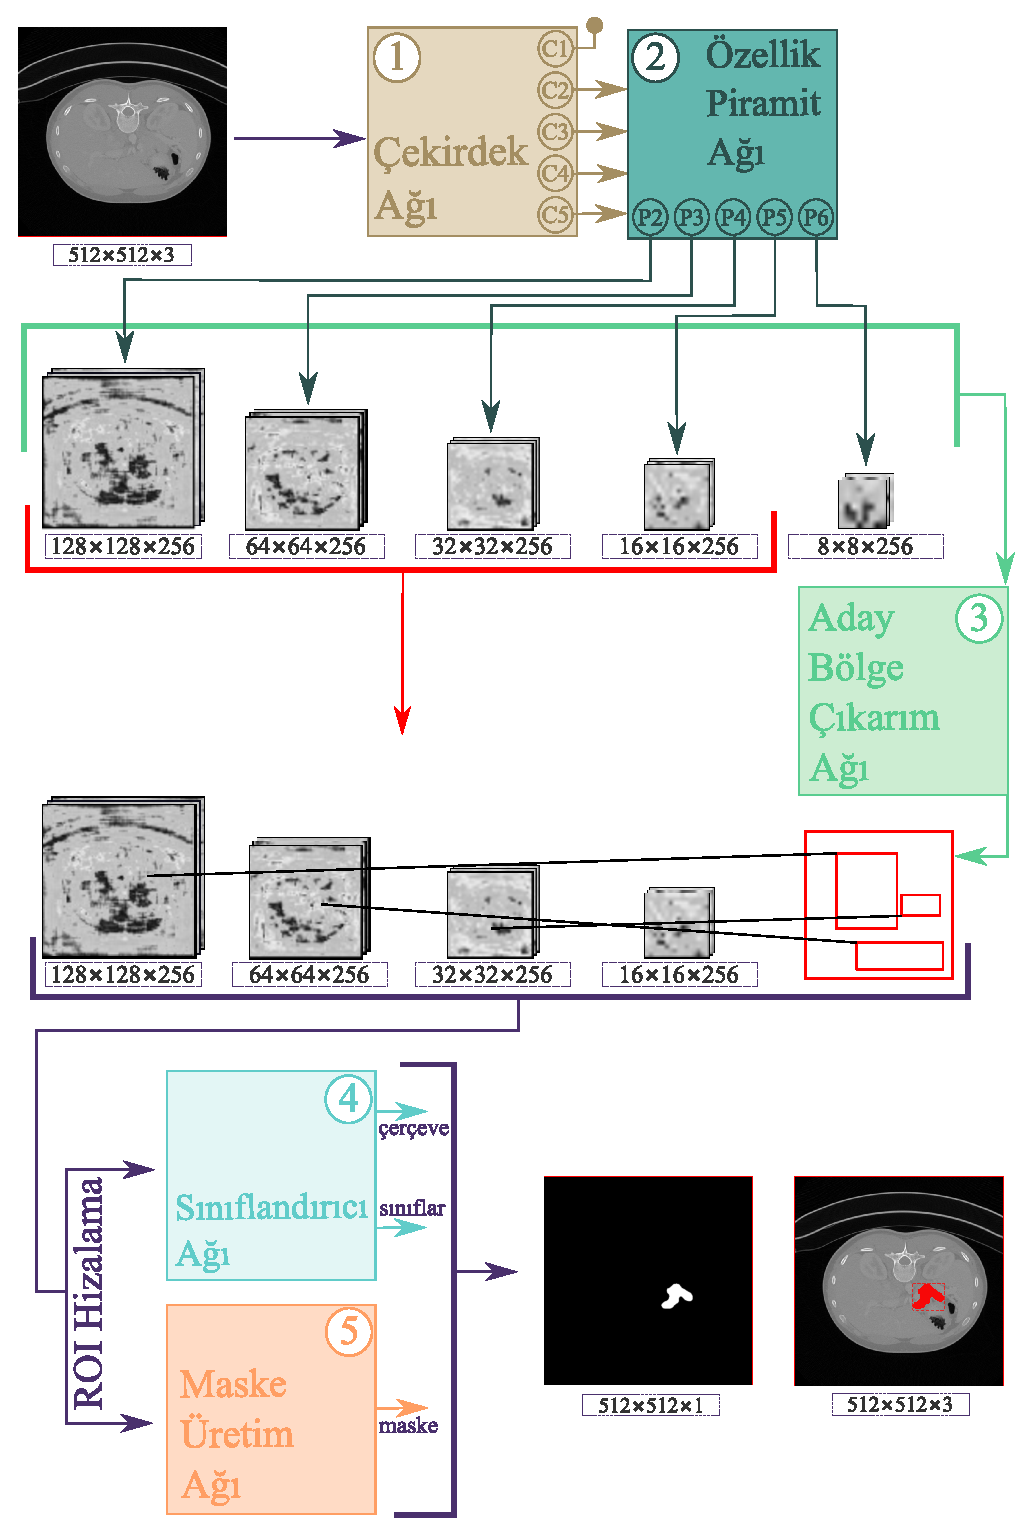
\includegraphics[scale=0.8]{Yapilan-Calismalar/Figures/maskrcnn.pdf}
		}
	\end{center}
\end{figure}

He tarafından 2018 yılında geliştirilen Mask R-CNN modeli \cite{he2017mask}, 2B nesne segmentasyonu için en güçlü yöntemlerden biridir. Bu model çok sınıflı nesne algılama için oldukça yüksek doğruluklu ve gerçek zamanlı performans sağlamaktadır. Bu model Hızlandırılmış Bölge Esaslı Konvolüsyonel Sinir Ağları \cite{ren2015faster} (Faster Region Proposal Convolutional Neural Network - Faster R-CNN) modelinin geliştirilmiş versiyonudur. Mask R-CNN modeli, Faster R-CNN modeline ek olarak maske üretimi ve sınıflandırıcı ağlardan oluşmaktadır. Mask R-CNN modelini diğer segmentasyon yöntemlerinden ayıran en önemli özelliği, görüntüdeki her nesnenin hem sınırlayıcı kutularını hem de segmentasyon sonuçlarını üretebilmesidir. 

Şekil \ref{fig:maskrcnn}’da Pankreas İlgi Bölgesinin Belirlenmesi fazının Mask R-CNN modeli kullanan ilk aşamasındaki beş ana adımın şematik gösterimi verilmektedir. Şekilde görüldüğü gibi Mask R-CNN modeli, Çekirdek Ağı (Head Network), Özellik Piramit Ağı (Feature Pyramid Network), Aday Bölge Çıkarım Ağı (Region Proposal Network), Sınıflandırıcı Ağı (Classifier Network) ve Maske Üretim Ağı (Mask Generation Network) olmak üzere beş ana adımdan oluşmaktadır. Pankreas İlgi Bölgesinin Belirlenmesi fazının Mask R-CNN modelini kullanan ilk aşamasında uygulanan ana adımlar şu şekilde açıklanabilmektedir.

\paragraph{Mask R-CNN Derin Ağ Modelinin Alt Ağlarından Çekirdek Ağı'nın Yapısı}

Kenar, doku ve renk kümesi bilgileri gibi 2B BT dilimlerinin spesifik özelliklerini tanımlamak için bu adımda Çekirdek Ağı (Head Network) oluşturulmaktadır. Bu tez çalışmasında Mask R-CNN Çekirdek Ağı olarak ResNet-101 CNN özellik çıkarıcı modelli ImageNet ağırlıkları ile transfer öğrenme tekniği kullanılarak denenmektedir. Tez çalışmasında kullanılan ResNet-101 modelli için Çekirdek Ağı'nın genel yapısı Şekil \ref{fig:head_network}’de verilmektedir. Bu ağ BT görüntüsünün tümünü $(512 \times 512 \times 3)$ giriş olarak almaktadır. Şekil \ref{fig:head_network}’de görüldüğü gibi giriş görüntüsünden C1, C2, C3, C4 ve C5 olarak adlandırılan beş farklı özellik haritası oluşturmaktadır. Bu özellik haritaları C1 için 128 x 128 x 64, C2 için 128 x 128 x 256, C3 için 64 x 64 x 512, C4 için 32 x 32 x 1024 ve C5 için 16 x 16 x 2048 olmak üzere farklı boyutlara sahiptirler. 

\captionsetup[figure]{margin={0.3cm,-2.5cm}}
\begin{figure}[h!]
	\begin{center}
		\vspace{0.4cm}
		\captionbox{ResNet-101 modeli kullanan Çekirdek Ağı'nın genel yapısı. \label{fig:head_network}}
		{
			\vspace{0.4cm}
			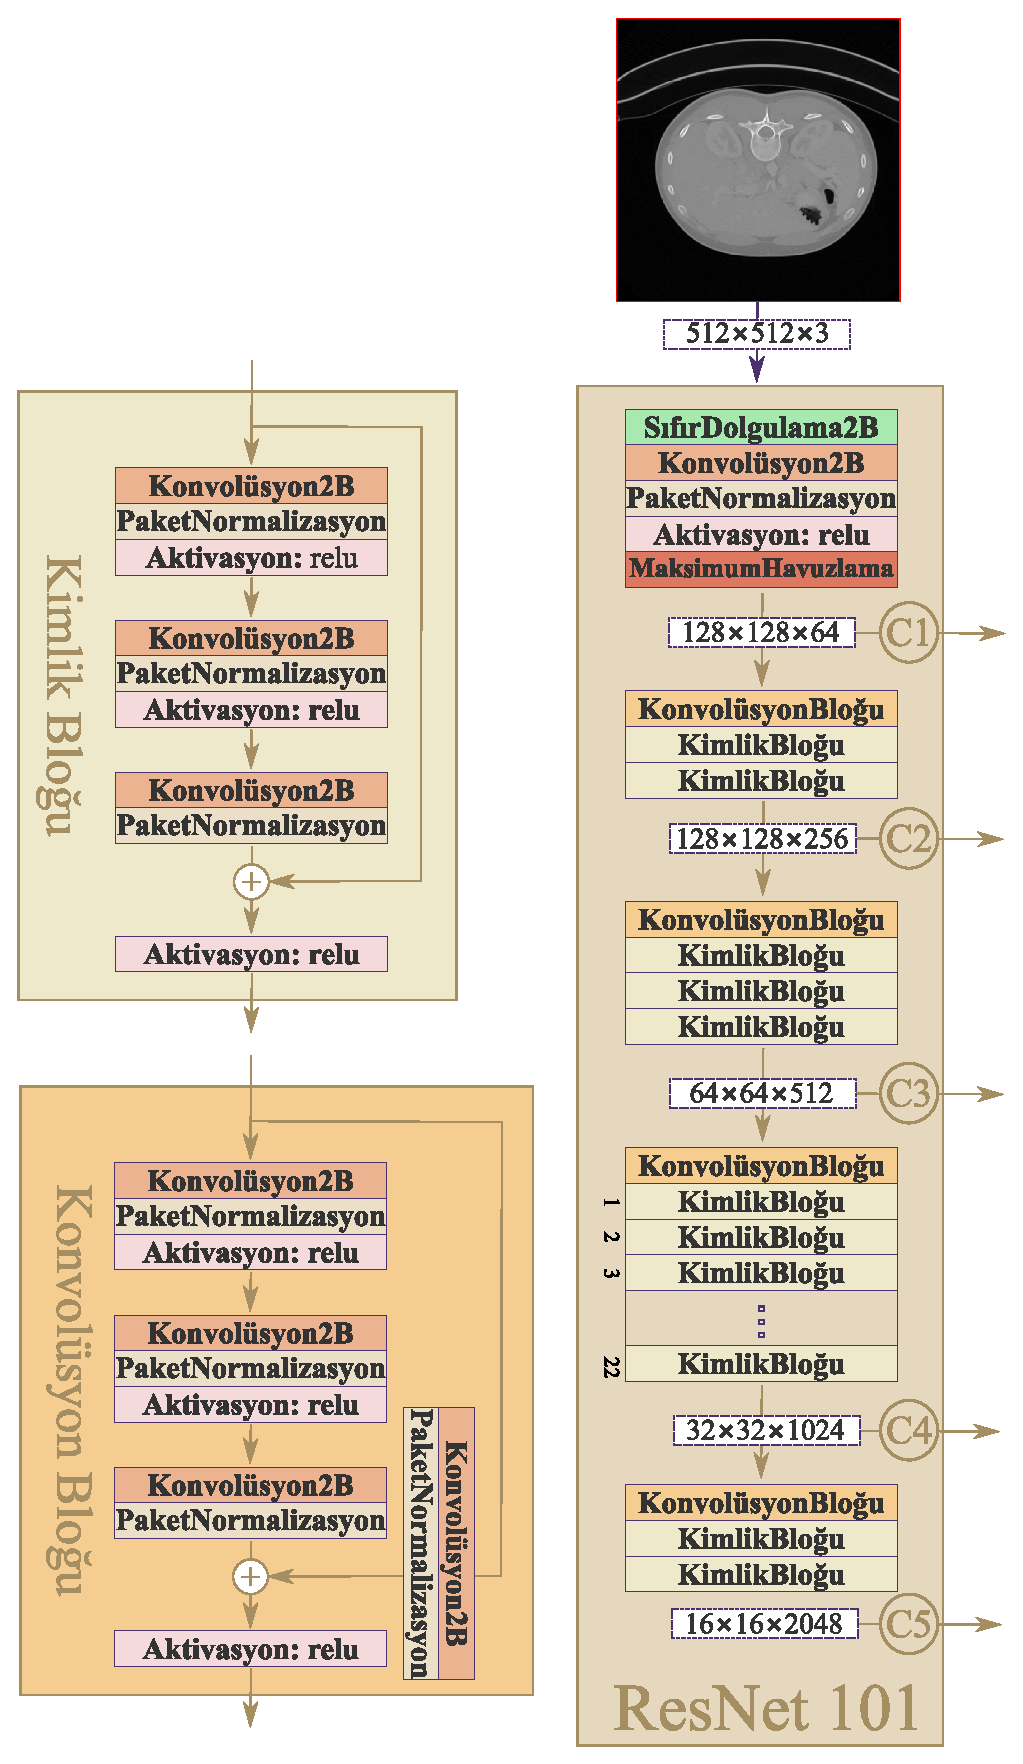
\includegraphics[scale=0.7]{Yapilan-Calismalar/Figures/head_network.pdf}
		}
	\end{center}
\end{figure}

ResNet mimarisi literatürde katman sayısını artırabilmek için artık (residual) bağlantıları kullanma fikri ile ortaya çıkarılmıştır \cite{he2016deep}. Böylece önceki katmanlardan gelen bilgi konvolüsyon işlemi sonrası katmanlarla birleştirilerek konvolüsyon işleminden kaynaklı bilgi kaybının önüne geçilebilmektedir. Eğitim hızını artırmak için Çekirdek Ağı'nda kullanılan ResNet-101 mimarisine transfer öğrenme tekniği kullanılarak ImageNet ağırlıkları ile ön yükleme işlemi gerçekleştirilmektedir. 

Çekirdek Ağı olarak kullanılan ResNet-101 mimarisi Şekil \ref{fig:head_network}’de görüldüğü gibi sıfır dolgulama (zero padding), 2B konvolüsyon (Convolutional), paket normalizasyon (Batch Normalization), doğrultulmuş doğrusal birim (RELU) ve maksimum havuzlama (Max Pooling) olmak üzere beş temel derin öğrenme katmanından oluşmaktadır. Ek olarak, Çekirdek Ağı'nda konvolüsyon (Convolutional) ve kimlik (identity) olmak üzere iki blok bulunmaktadır. Konvolüsyon ve kimlik blokları 2B konvolüsyon, paket normalizasyon ve RELU katmanlarını içermektedirler. Bu bloklar paket normalizasyonu katmanının çıkışına giriş ekleyerek kaybolan gradyan problemini ortadan kaldırmaktadırlar \cite{he2016deep}.

\paragraph{Mask R-CNN Derin Ağ Modelinin Alt Ağlarından Özellik Piramit Ağı'nın Yapısı}

Farklı ölçeklerde nesneleri algılamak nesne ölçeği azaldıkça zorlaşmaktadır. Bu amaçla görüntünün farklı ölçeklerdeki piramiti oluşturularak nesne tespiti farklı ölçeklerde gerçekleştirilebilmektedir. Farklı ölçeklerdeki görüntü piramitlerini işlemek oldukça fazla işlemci zamanı ve bilgisayar belleği tüketilmesine sebep olmaktadır. Bunun yerine görüntünün farklı ölçeklerdeki özellik haritalarında bu işlemi gerçekleştirmek çok daha efektif olmaktadır. Özellik Piramit Ağı (Feature Pyramid Network - FPN) bu amaç için geliştirilmiş derin özellik çıkarım modelidir \cite{lin2017feature}.  

\captionsetup[figure]{margin={0.5cm,-3cm}}
\begin{figure}[h!]
	\begin{center}
		\vspace{0.4cm}
		\captionbox{Özellik Piramit Ağı'nın genel  yapısı.\label{fig:feature_pyramid_network}}
		{
			\vspace{0.4cm}
			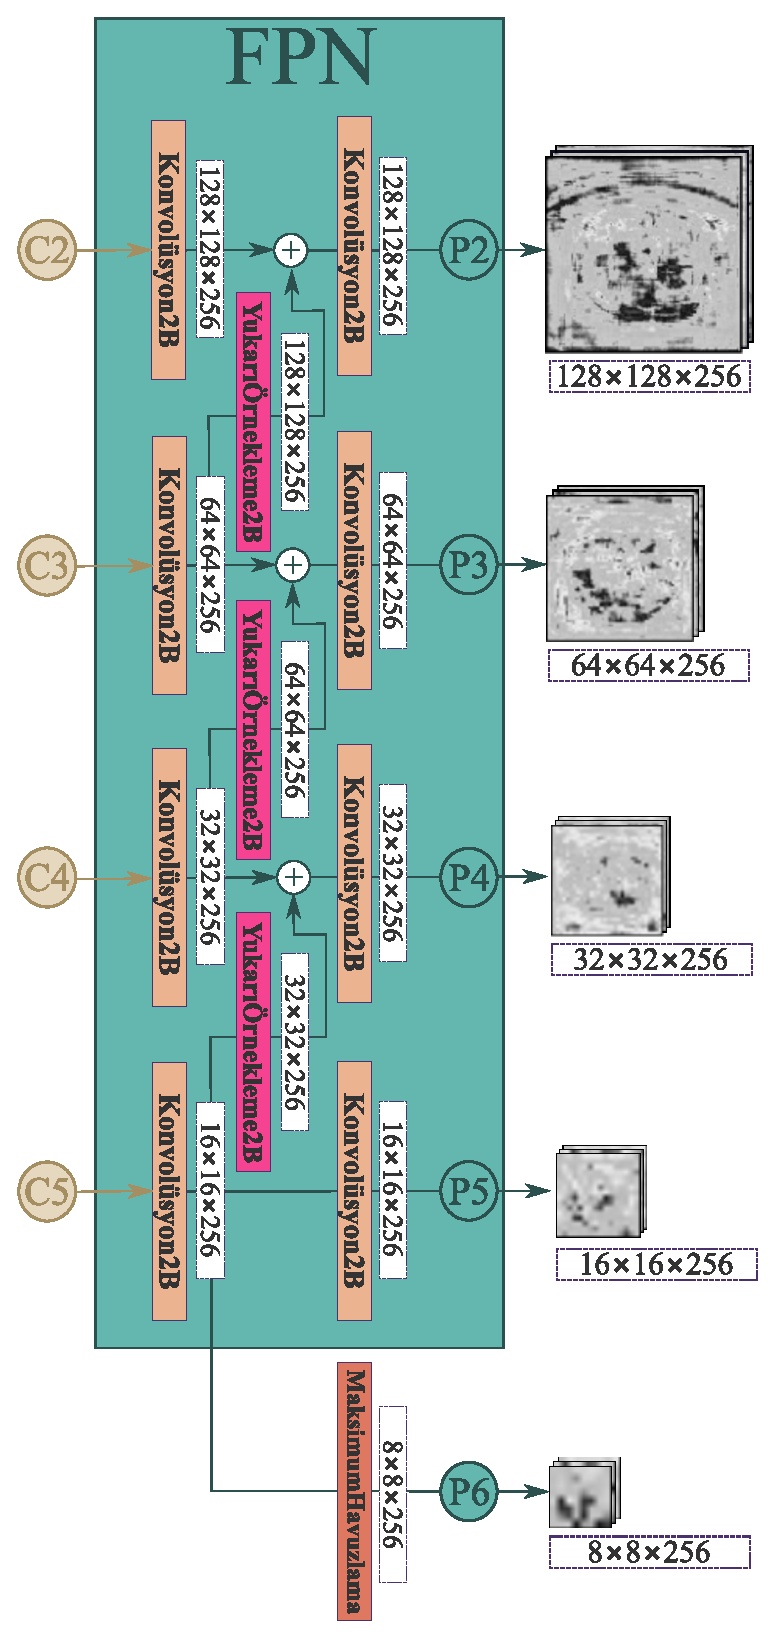
\includegraphics[scale=0.72]{Yapilan-Calismalar/Figures/feature_pyramid_network.pdf}
		}
	\end{center}
\end{figure}

2B BT dilimlerinin daha belirgin özelliklerini çıkarmak için, bu adımda Özellik Piramit Ağı oluşturulmaktadır. Özellik Piramit Ağı'nın genel yapısı Şekil \ref{fig:feature_pyramid_network}’de verilmektedir. Şekil \ref{fig:feature_pyramid_network}’de görüldüğü gibi Özellik Piramit Ağı, Çekirdek Ağı tarafından üretilen ($C2$ - $128 \times 128 \times 256$, $C3$ - $64 \times 64 \times 512$, $C4$ - $32 \times 32 \times 1024$ ve $C5 - 16 \times 16 \times 2048)$ dört farklı özellik haritasını giriş olarak almaktadır. Bu ağ yukarıdan aşağı yol (top-down pathway) adı verilen bir yaklaşım kullanarak beş farklı piramit özellik haritasını ($P2$ - $128 \times 128 \times 256$, $P3$ - $64 \times 64 \times 256$, $P4$ - $32 \times 32 \times 256$, $P5 - 16 \times 16 \times 256$ ve $P6$ - $8 \times 8 \times 256$) çıktı olarak üretmektedir. Yukarıdan aşağı yol yaklaşımında, yukarı ölçekli operasyonlar en küçük ölçekli özellik haritasından ($C5$) başlayarak en büyük ölçekli özellik haritasına doğru uygulanmaktadır. Yukarıdan aşağı yol yaklaşımı Çekirdek Ağı'nın farklı ölçeklerdeki konvolüsyon özellik haritalarını temsil etmektedir. Serideki özellik haritası sayısını $256$’ya düşürmek için Şekil \ref{fig:feature_pyramid_network}’de verildiği gibi ilk olarak Çekirdek Ağı’nda üretilen özellik haritaları ($C2$, $C3$, $C4$ ve $C5$) $1 \times 1$ ölçekli bir filtre ile konvolüsyona tabi tutulmaktadır. Daha sonra, serideki yukarı örneklenmiş özellik haritaları önceki özellik haritalarına eklenmektedir. Nihai özellik haritalarını ($P2$ - $128 \times 128 \times 256$, $P3$ - $64 \times 64 \times 256$, $P4$ - $32 \times 32 \times 256$ ve $P5$ - $16 \times 16 \times 256$) elde etmek için $3 x 3$ boyutundaki konvolüsyon filtresi bir önceki işlemin tüm sonuçlarına  uygulanmaktadır. $P6$ ($8 \times 8 \times 256$) özellik haritası ise maksimum havuzlama işlemi ile $C5$ girişinden üretilmektedir.

\paragraph{Mask R-CNN Derin Ağ Modelinin Alt Ağlarından Aday Bölge Çıkarım Ağı'nın Yapısı}

Aday Bölge Çıkarım Ağı (Region Proposal Network - RPN), nesneler için bölge teklifleri oluşturmaktadır. Aday Bölge Çıkarım Ağı kendi içinde özel ve benzersiz bir mimariye sahiptir. Piramit özellik haritalarından dikdörtgensel nesne önerileri üretmek için Aday Bölge Çıkarım Ağı tasarlanmaktadır. Aday Bölge Çıkarım Ağı'nın genel yapısı Şekil \ref{fig:region_proposal_network}’te verilmektedir. 

\captionsetup[figure]{margin={0.5cm,-3cm}}
\begin{figure}[h!]
	\begin{center}
		\vspace{0.4cm}
		\captionbox{Aday Bölge Çıkarım Ağı'nın genel yapısı.\label{fig:region_proposal_network}}
		{
			\vspace{0.4cm}
			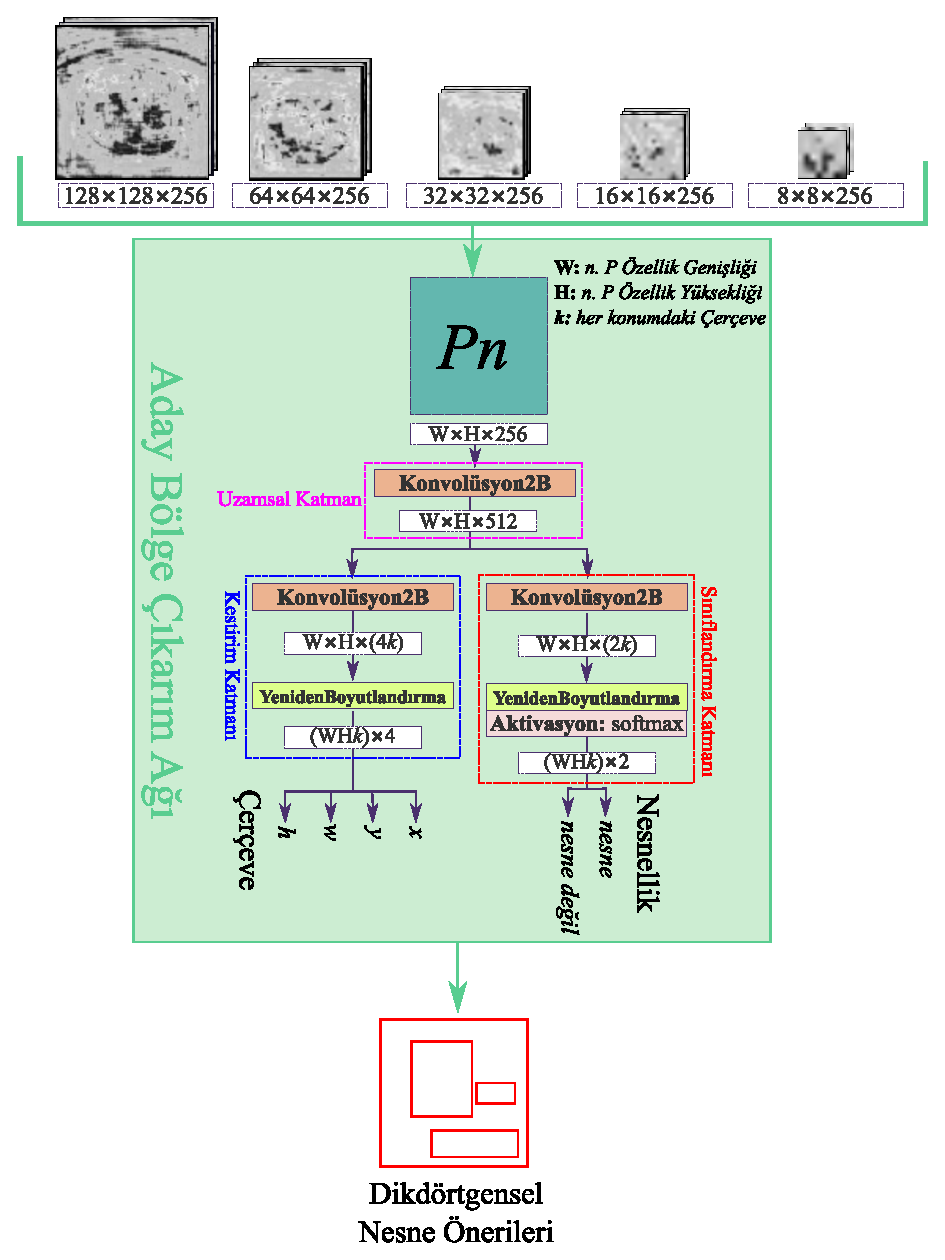
\includegraphics[scale=0.75]{Yapilan-Calismalar/Figures/region_proposal_network.pdf}
		}
	\end{center}
\end{figure}

Aday Bölge Çıkarım Ağı giriş olarak Özellik Piramit Ağı tarafından üretilen beş farklı özellik haritasını ($P2$ - $128 \times 128 \times 256$, $P3$ - $64 \times 64 \times 256$, $P4$ - $32 \times 32 \times 256$ ve $P5$ - $16 \times 16 \times 256$) almaktadır. Aday Bölge Çıkarım Ağı temelde üç farklı ana katmandan oluşmaktadır. Tasarlanan ağın ilk katmanında (Uzamsal katman - Spatial layer) piramit özellik haritaları boyutu $3 \times 3$ olan bir uzamsal filtre ile konvolüsyona tabi tutulmaktadır. Her bir piramit özellik haritası konumunda aynı anda birden çok nesne tahmini öngörülmektedir. Şekil \ref{fig:region_proposal_network}’te görülen k, piramit özellik haritasındaki her bir konum için mümkün olan maksimum öneri sayısını (anchor olarak adlandırılır) belirtmektedir. Uzamsal katmandan sonra, ilk katmanın çıkışlarına $1 \times 1$ filtre boyutuna sahip iki konvolüsyon katmanı uygulanmaktadır. Bu iki konvolüsyon katmanı regresyon ve sınıflandırıcıdır. Regresyon katmanı, k tane çerçevenin (anchor) koordinatlarını temsil eden $(WHk) \times 4$ çıkış değerine sahiptir. Bu değerler bulunan dikdörtgensel bölgenin koordinatlarını temsil etmektedir. Sınıflandırıcı katman bir softmax’ın ardından $(WHk) \times 2$ tane dikdörtgensel bölgenin nesne olup olmadığını göstermektedir.  $W \times H$ boyutuna sahip bir piramit özellik haritası için, Aday Bölge Çıkarım Ağı tarafından üretilen dikdörtgensel bölgelerin sayısı $W \times H \times k$’dır.

\paragraph{Mask R-CNN Derin Ağ Modelinin Alt Ağlarından Sınıflandırıcı Ağı'nın Yapısı}
2B BT dilimindeki pankreas bölgesinin kaba konumunu tespit etmek için bu adımda Sınıflandırıcı Ağı (Classifier Network) tasarlanmaktadır. Sınıflandırıcı Ağı'nın genel yapısı Şekil \ref{fig:classifier_network}’te verilmektedir. Sınıflandırıcı Ağı giriş olarak Aday Bölge Çıkarım Ağı tarafından üretilen dikdörtgensel nesne önerilerini ($P2$, $P3$, $P4$ ve $P5$) almaktadır. İlk olarak Piramit İlgi Bölgesi Hizalama (Pyramid ROI Align) Özellik Piramit Ağı tarafından üretilen piramit özellik haritalarını ($P2$ - $128 \times 128 \times 256$, $P3$ - $64 \times 64 \times 256$, $P4$ - $32 \times 32 \times 256$ ve $P5$ - $16 \times 16 \times 256$) Aday Bölge Çıkarım Ağı tarafından çıkarılan dikdörtgensel bölgeleri sınıflandırmaya tabi tutulabilmek için ($7 \times 7 \times 256$) çözünürlüğüne dönüştürmektedir. Daha sonra, $7 \times 7 \times 256$ çözünürlüklü her bir dikdörtgen nesne aday bölgesine $1$ konvolüsyon, $1$ paket normalizasyonu (batch normalizasyonu - BN) ve $1$ ReLU katmanları içeren blok iki kez uygulanmaktadır.  Her bir dikdörtgen nesne aday bölgesi için sabit boyutlu ($1 \times 1 \times 1024$) özellik vektörleri elde edilmektedir. Sondaki yoğun (dense) katmanlar sıkıştırılmış özellik vektörlerini girdi olarak almaktadırlar. Bu katmanlar her kaba pankreas bölgesi için sınıflandırma sonucu (pankreas ve pankreas olmayan) ve son nesne dikdörtgensel bölgesi koordinatlarını ($x,y,w,h$) gösteren çıktılar üretmektedir.

\captionsetup[figure]{margin={0.5cm,-3cm}}
\begin{figure}[h!]
	\begin{center}
		\vspace{0.4cm}
		\captionbox{Sınıflandırıcı Ağ'ın genel yapısı.\label{fig:classifier_network}}
		{
			\vspace{0.4cm}
			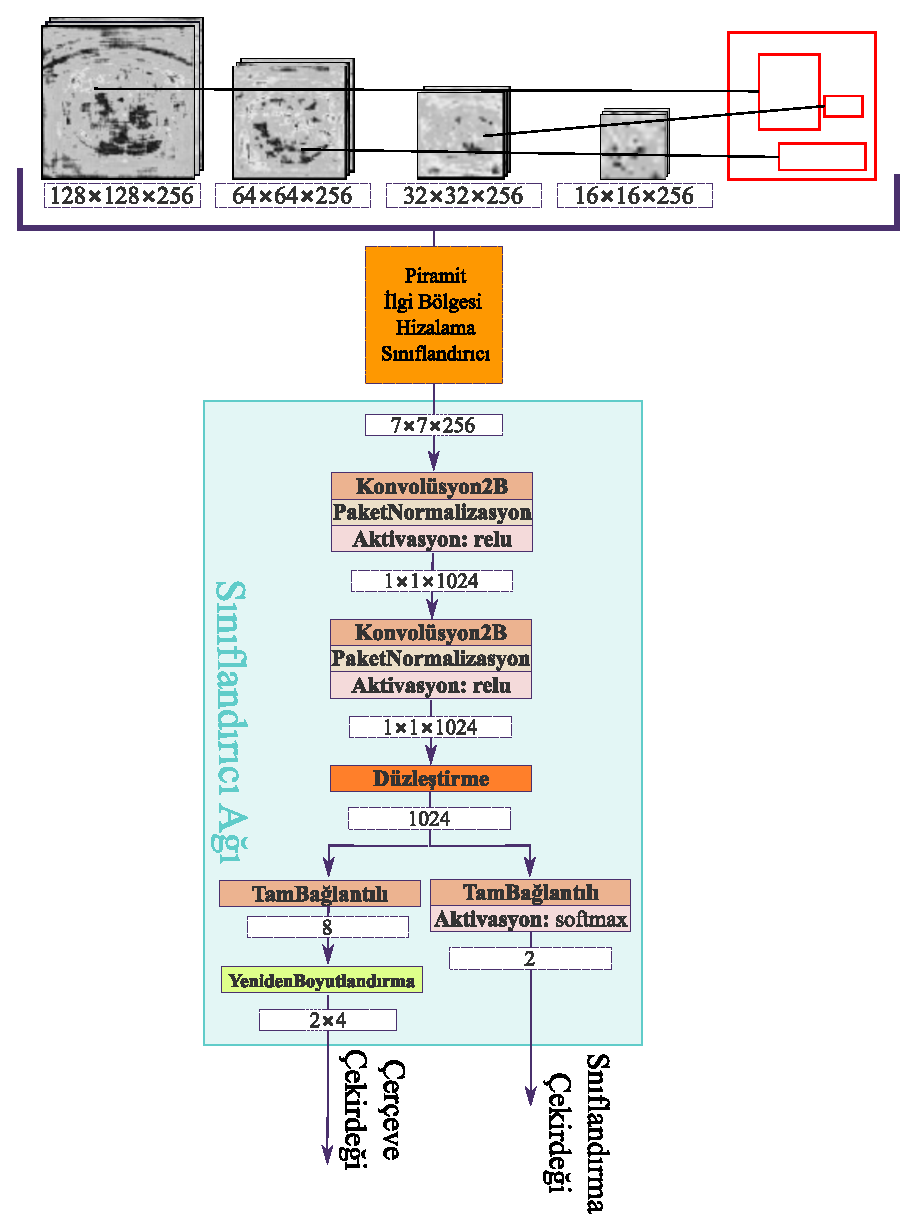
\includegraphics[scale=0.88]{Yapilan-Calismalar/Figures/classifier_network.pdf}
		}
	\end{center}
\end{figure}

\paragraph{Mask R-CNN Derin Ağ Modelinin Alt Ağlarından Maske Üretim Ağı'nın Yapısı}

\captionsetup[figure]{margin={0.5cm,-3cm}}
\begin{figure}[h!]
	\begin{center}
		\vspace{0.4cm}
		\captionbox{Maske Üretim Ağı'nın genel yapısı.\label{fig:mask_generation_network}}
		{
			\vspace{0.4cm}
			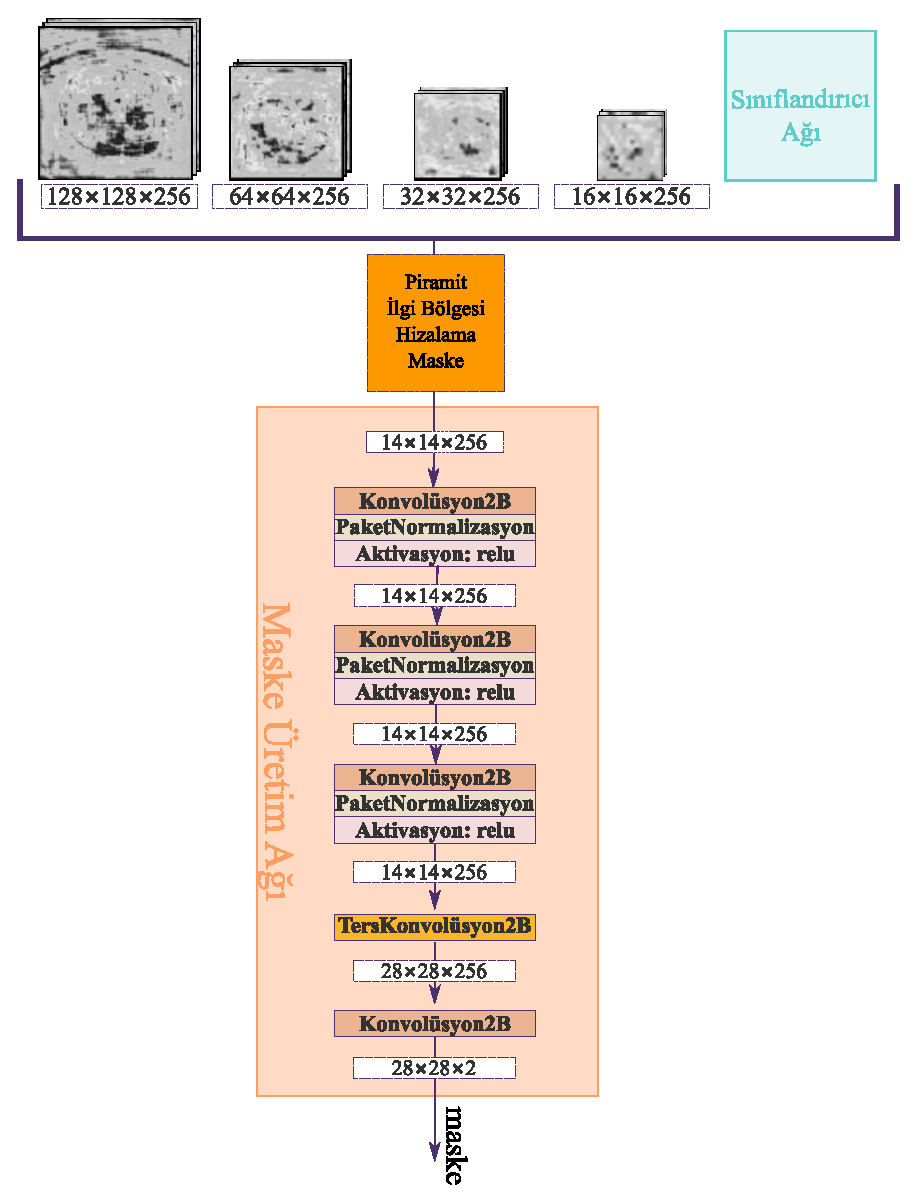
\includegraphics[scale=0.88]{Yapilan-Calismalar/Figures/mask_generation_network.pdf}
		}
	\end{center}
\end{figure}

2B BT diliminde algılanan pankreas bölgesinin sınırlayıcı çerçevesi içinde pankreas bölgesinin (maske) segmentasyonu için Maske Üretim Ağı (Mask Generation Network - MGN) tasarlanmaktadır. Sınıflandırıcı Ağı'ndan gelen pankreas çerçeve bölgeleri üzerinde Özellik Piramit Ağı tarafından üretilen P2, P3, P4, P5 özellik haritaları kullanılarak pankreas bölgesinin kaba sınırları tespiti hedeflenmektedir. Maske Üretim Ağı'nın genel yapısı Şekil \ref{fig:mask_generation_network}’te gösterilmektedir. Maske Üretim Ağı, Özellik Piramit Ağı tarafından üretilen özellik haritalarını ($P2$, $P3$, $P4$ ve $P5$) ve Sınıflandırıcı Ağı tarafından tahmin edilen pankreas dikdörtgensel bölgelerini girdi olarak almaktadır. İlk olarak, Piramit İlgi Bölgesi Hizalama ile girişler aynı çözünürlüğe ($14 \times 14 \times 256$) dönüştürülmektedir. Daha sonra $14 \times 14 \times 256$ çözünürlüklü her özellik haritasına $1$ konvolüsyon, $1$ paket normalizasyonu ve $1$ ReLU katmanlarını içeren blok üç kez uygulanmaktadır. Son konvolüsyon katmanı, transpoze edilen özellik haritalarını girdi olarak almaktadır. Bu katman her pankreas bölgesinin sınırlayıcı kutusunu (maskesini) gösteren bir çıktı oluşturmaktadır.

\subsubsection{Kaba Pankreas Bölgesinin Mask R-CNN'den Elde Edilen Merkez Bilgisi ile Belirlenmesi}

\captionsetup[figure]{margin={0.3cm,-3cm}}
\begin{figure}[h!]
	\begin{center}
		\vspace{0.4cm}
		\captionbox{Kaba Pankreas Bölgesi Çıkarılması aşamasının şematik temsili.\label{fig:center_of_mass}}
		{
			\vspace{0.4cm}
			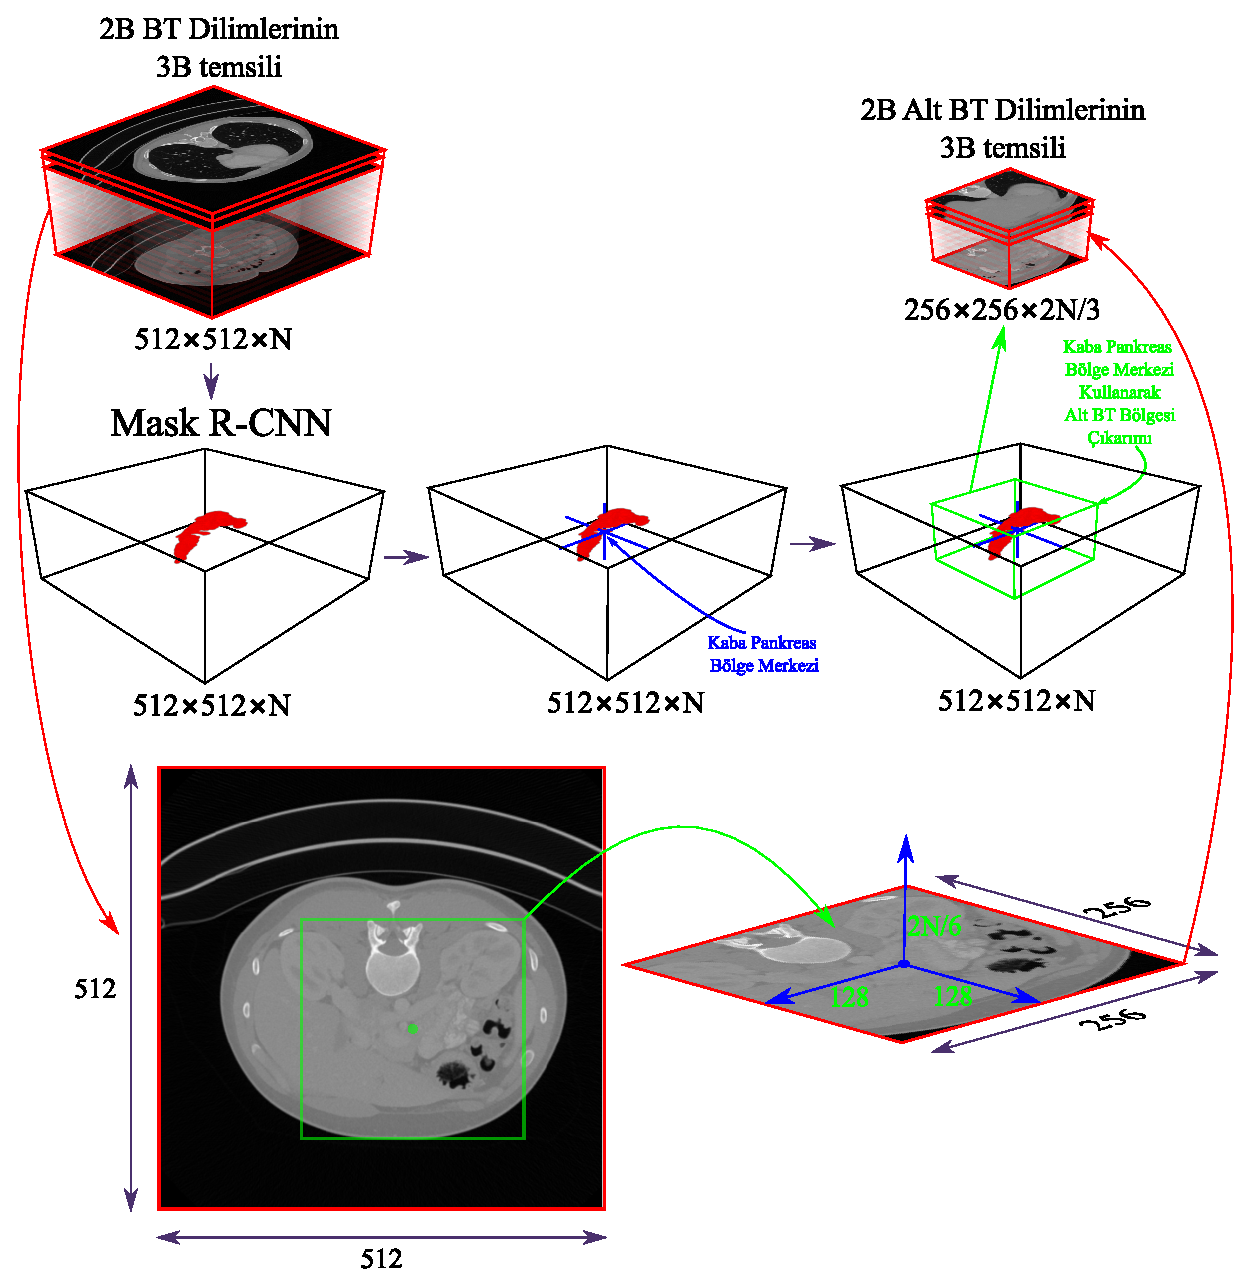
\includegraphics[scale=0.61]{Yapilan-Calismalar/Figures/center_of_mass.pdf}
		}
	\end{center}
\end{figure} 

Pankreas İlgi Bölgesinin Belirlenmesi fazının ikinci aşaması olan Kaba Pankreas Bölgesinin Çıkarılması, Belirlenen İlgi Bölgesinde Pankreas Segmentasyonu fazı için işlenen BT dilimlerinin boyutunu azaltmayı amaçlamaktadır. Kaba Pankreas Bölgesinin Çıkarılması aşaması, ilk aşamada Mask R-CNN modeli ile üretilen kaba pankreas bölgelerini giriş olarak almaktadır. Şekil \ref{fig:center_of_mass}’da Kaba Pankreas Bölgesinin Çıkarılması aşamasının şematik temsili verilmektedir. Şekil \ref{fig:center_of_mass}’da gösterildiği gibi, ilk olarak maskelenmiş 2B BT dilimleri ($512 \times 512 \times N$) üzerindeki pankreas bölgesinin merkezi Eşitlik \ref{eq:centerofmass} ile hesaplanmaktadır.
\begin{equation}
	\label{eq:centerofmass}
	\left(x_{c}, y_{c}, z_{c}\right)=\frac{1}{N} \sum_{i=1}^{N}\left(x_{i}, y_{i}, z_{i}\right)
\end{equation}

Eşitlik \ref{eq:centerofmass}’de $\left(x_{c}, y_{c}, z_{c}\right)$ kaba pankreas bölgesinin merkezini, $\left(x_{i}, y_{i}, z_{i}\right)$ kaba pankreas bölgesindeki noktaların koordinatlarını ve N kaba pankreas bölgesindeki noktaların sayısını temsil etmektedir. Kaba pankreas bölge merkezinin hesaplanmasından sonra, her bir BT dilimindeki ($512 \times 512$) 3B kümeden elde edilen kaba merkezin etrafındaki bölge kırpılarak 2B alt BT dilimleri ($256 \times 256 \times 2N / 3$) çıkarılmaktadır. Bu bölge, x ve y eksenlerinin sol ve sağ yönlerinde 128 piksel ve z ekseninin alt ve üst yönlerinde 2N/6 dilimlerinin hareket ettirilmesiyle oluşturulmaktadır; burada x, y, z, kaba pankreas bölgesinin 3B merkez koordinatlarını, $N$ BT dilimlerinin sayısını göstermektedir.

\subsection{Belirlenen İlgi Bölgesinde Pankreas Segmentasyonu}
Mask R-CNN modeli, nesne kaba hatlarını bulmak için oldukça uygun bir algoritmadır. Fakat hatlarının çok değişken olduğu nesnelerin sınır tespiti için yeterince başarılı olamamaktadır. Bunun en temel sebebi nihai maskeleme aşamasında hesaplama yükünü azaltmak için tüm aday bölgelerin $14 \times 14$ çözünürlüğüne düşürülmesidir. Bu nedenle Mask R-CNN modeli nesnenin kaba hatlarını çıkarmada oldukça başarılı olsa da nesne sınırlarının daha doğru belirlenebilmesi için daha detaylı bir yaklaşım gerekmektedir.

Önerilen çalışmada giriş olarak verilen 2B BT dilimlerinin ($512 \times 512 \times N$) tümünü işlemek yerine, ikinci faz (Belirlenen İlgi Bölgesinde Pankreas Segmentasyonu) aday pankreas bölgesini kapsayan 2B alt BT dilimlerini ($256 \times 256 \times 2N/3$) kullanmaktadır. Bu sayede, daha tatmin edici sonuçlar elde edilmekte, otomatik pankreas segmentasyonu için hesaplama karmaşıklığı ve maliyeti azaltılmaktadır. Bu faz, 3B U-Net modelini kullanarak aday pankreas bölgesini içeren 2B alt BT dilimleri tekrar düzenlemeyi amaçlamaktadır. Tasarlanan modelde, önceki fazda (Pankreas İlgi Bölgesinin Belirlenmesi) üretilen 2B alt BT dilimleri ($256 \times 256 \times 2N/3$) giriş olarak alınmaktadır. Pankreas bölgesinin segmente edilmiş 2B alt BT dilimleri ($256 \times 256 \times 2N/3$) çıkış olarak üretilmektedir. Pankreas Segmentasyon fazı ön işlem (pre - processing), 3B U-Net, son işlem (post-processing) ve geri montajlama (decropping) olmak üzere dört adımdan oluşmaktadır. Şekil \ref{fig:3dunet1} Pankreas Segmentasyon fazında kullanılan 3B U-Net modelinin şematik temsilini göstermektedir. Bu model, kodlayıcı (Şekil \ref{fig:3dunet1}'de aşağı yönlü sol taraf) ve kod çözücü (Şekil \ref{fig:3dunet1}'de yukarı yönlü sağ taraf) olmak üzere iki temel aşamadan oluşmaktadır. Pankreas Segmentasyonu fazında uygulanan bu adımların detayları bundan sonraki alt başlıklarda daha ayrıntılı verilecektir. 

\captionsetup[figure]{margin={0.4cm,-2cm}}
\begin{figure}[h!]
	\begin{center}
		\vspace{0.4cm}
		\captionbox{Pankreas Segmentasyon fazında kullanılan 3B U-Net modelinin şematik temsili. \label{fig:3dunet1}}
		{
			\vspace{0.4cm}
			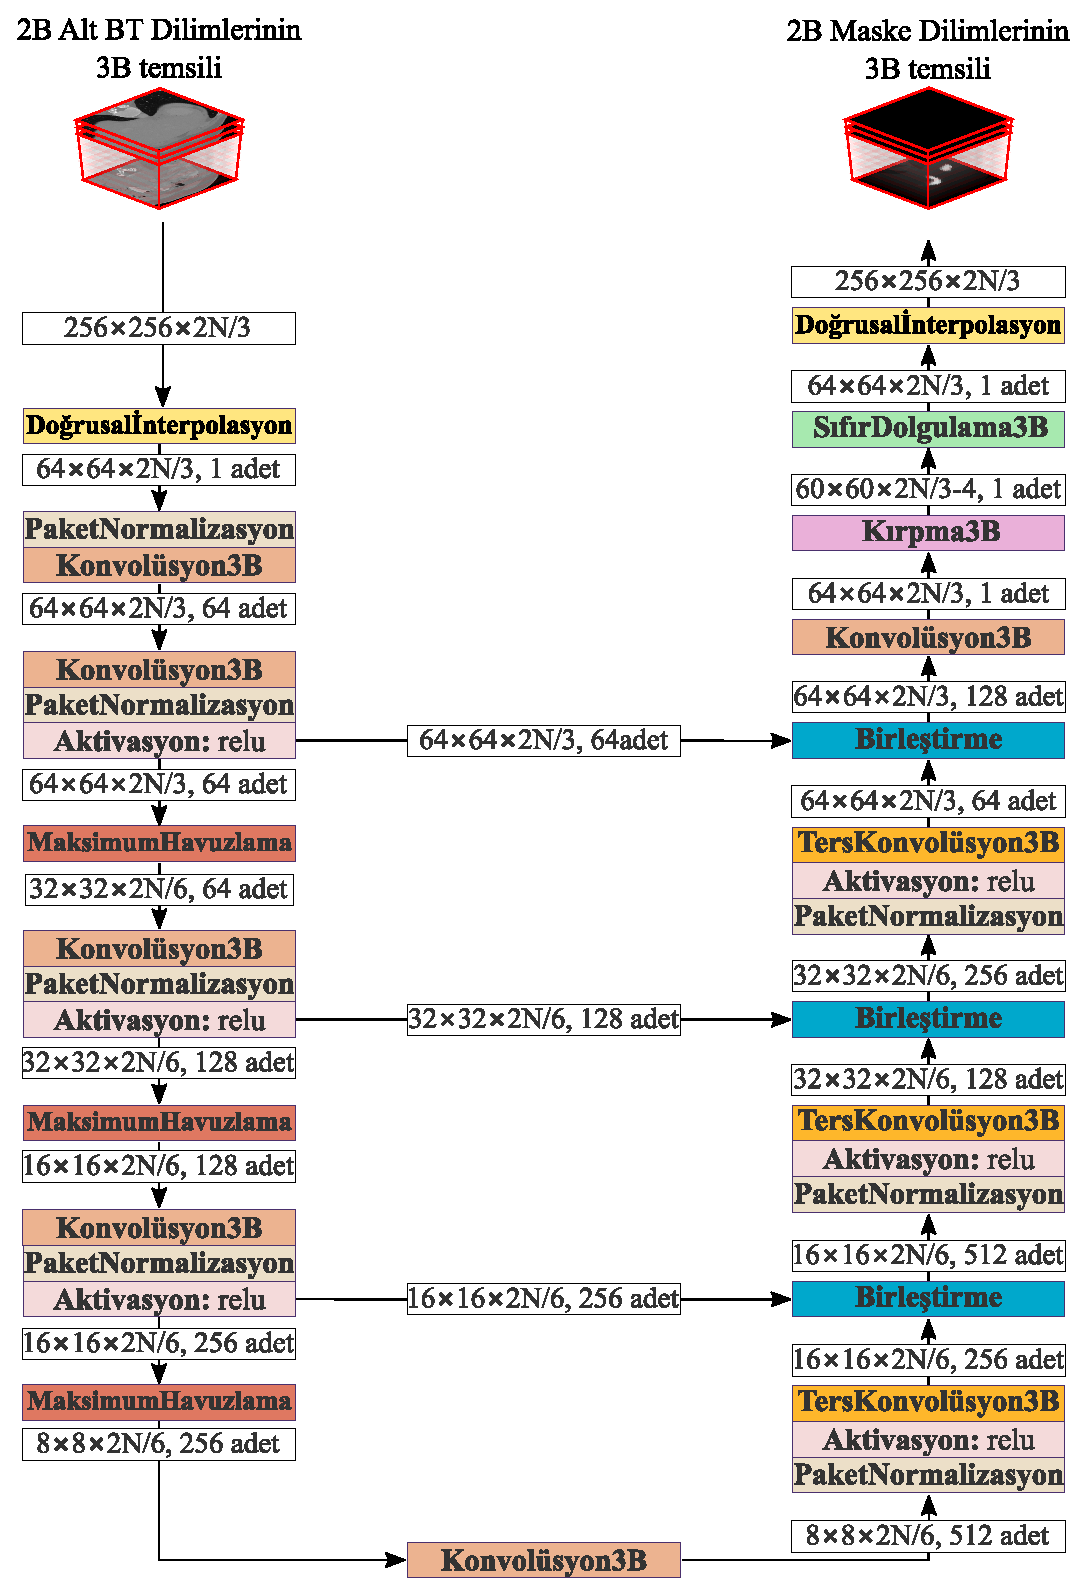
\includegraphics[scale=0.6]{Yapilan-Calismalar/Figures/3dunet.pdf}
		}
	\end{center}
\end{figure} 

\subsubsection{Pankreas Segmentasyonu İçin Ön İşlem}
Belirlenen İlgi Bölgesinde Pankreas Segmentasyonu fazında 3B U-Net modelini uygularken GPU bellek tüketimini azaltmak için önceki fazda (Pankreas İlgi Bölgesinin Belirlenmesi) oluşturulan 2B alt BT dilimlerinin boyutu ($256 \times 256 \times 2N/3$) yerine ($64 \times 64 \times 2N/3$) olarak yeniden boyutlandırılmaktadır.

\subsubsection{Pankreas Segmentasyonunun 3B U-Net Modeli ile Gerçekleştirilmesi}
3B U-Net modeli, kodlayıcı ve kod çözücü olmak üzere iki temel aşamadan oluşmaktadır. Bu iki temel aşama şu şekilde açıklanabilmektedir:

\paragraph{3B U-Net Modeli Kodlayıcı Aşaması}
Kodlayıcı aşamasının temel amacı, aday pankreas bölgesinden küresel karakteristikleri çıkarmaktır. Bu aşama, bir önceki fazda üretilen pankreasın kaba olarak segmente edilmiş 2B alt BT dilimlerinin ($256 \times 256 \times 2N / 3$) işlem yükünü azaltmak için yeniden boyutlandırılmış versiyonu olan 2B alt BT dilimlerini ($64 \times 64 \times 2N / 3$) giriş veri seti olarak almaktadır. Tasarlanan modelde, 1 konvolüsyon, 1 paket normalizasyon, 1 ReLU aktivasyon ve 1 maksimum havuzlama katmanlarını içeren üç bölüm bulunmaktadır. Bu üç bölümden önce, ($64 \times 64 \times 2N / 3$) boyutundaki giriş katmanına ($1, 4, 4$) çekirdek boyutlu 1 konvolüsyon, 1 paket normalizasyonu ve 1 ReLU aktivasyon işlemleri uygulanmaktadır. Literatür çalışmalarında küçük boyutlu konvolüsyon filtrelerinin daha iyi performans sağladığı gösterilmektedir. Bu nedenle, bu modelin tüm bölümlerindeki konvolüsyon katmanlarının 3B filtre büyüklükleri $3 \times 3 \times 3$ olarak alınmaktadır. Konvolüsyon katmanından sonra çıkış değerleri paket normalizasyonu katmanıyla normalleştirilmektedir. Eğitimi hızlandırmak ve eğrilik geri yayılımını sağlamak için katmanlarda ReLU aktivasyonu uygulanmaktadır. Tüm bölümlerin sonunda, maksimum havuzlama katmanı tasarlanan modelin hesaplama ve karmaşıklık maliyetlerini azaltmak için önceki katmanlarda üretilen çıktıları alt örneklemektedir. İlk bloktaki maksimum havuzlama katmanının filtre boyutu ($2 \times 2 \times 2$), diğer bloklardaki maksimum havuzlama katmanlarının filtre boyutundan ($1 \times 2 \times 2$) farklıdır. Buradaki amaç 3B maksimum havuzlama filtresinin ilk elemanının 3B BT görüntüsündeki dilim sayısına etki etmesidir. Bu değerin ilk blokta $2$ olması BT görüntülerinin dilim sayısı ve hesaplama maliyetini düşürmektedir. Fakat diğer bloklarda bu sayı $1$ değerine sabitlenerek 3B uzayda dilim sayısı azaltılmakta ve maskeleme sonucunun bozulmasının önüne geçilmektedir.

\paragraph{3B U-Net Modeli Kod Çözücü Aşaması}
3B U-Net modeli Kod Çözücü aşaması, Kodlayıcı aşamasında öğrenilen özellikleri kullanarak ($64 \times 64 \times 2N / 3$) boyutuna sahip pankreas segmentasyon sonuçlarını oluşturmaktadır. Tasarlanan modelde $1$ paket normalizasyonu, 1 ReLU, 1 ters konvolüsyon ve 1 birleştirme katmanlarını içeren üç bölüm bulunmaktadır. Konvolüsyon katmanının aksine, ters konvolüsyon katmanları küresel karakteristiklerin boyutunu arttırmaktadır. Tüm bölümlerdeki ters konvolüsyon katmanlarının filtre boyutları $3 \times 3 \times 3$ olarak atanmaktadır. Ters konvolüsyon katmanından sonra, atlama bağlantıları ile birleştirme işlemi kodlayıcı aşamasından yüksek çözünürlüklü global özellikler sağlamaktadır. Tüm bölümlerin sonundaki konvolüsyon, kırpma ve sıfır dolgulama katmanları segmente edilmiş pankreas bölgelerini üretmektedirler. Şekil \ref{fig:3dunet1}'de gösterildiği gibi, son konvolüsyon katmanının aktivasyon fonksiyonu olarak Sigmoid aktivasyon fonksiyonu kullanılmaktadır. Sigmoid aktivasyon fonksiyonu 0 ile 1 arasında çıktılar üretmektedir. Ek olarak, ikili çapraz entropi (binary cross-entropy) kayıp fonksiyonu olarak kullanılmaktadır. Bu sayede önerilen model piksel değerleri $0$ ile $1$ arasında değişen $2N/3$ adet $64 \times 64$ görüntü üretmektedir.

\subsubsection{Pankreas Segmentasyonu İçin Son-işlem (Post - processing)}
Önceki adımda 3B U-Net modeli ile oluşturulan $2N/3$ adet $64 \times 64$ boyutuna sahip görüntü, piksel değerleri $0$ ile $1$ arasında olan olasılık haritalarını temsil etmektedir. Bu adımda, olasılık haritalarında pankreas veya pankreas dışı bölgenin belirlenmesi için öncelikle Sert Eşikleme (Hard Thresholding) işlemi uygulanmaktadır. Bu işlem için eşik değeri $0,5$ olarak kabul edilmektedir. Bu nedenle $0,5$'ten büyük piksel değerleri pankreas bölgesini ($1$) belirtirken, diğer değerler pankreas dışı bölgeler ($0$) olarak kabul edilmektedir. Daha sonra pankreas veya pankreas dışı bölgeyi ($64 \times 64 \times 2N/3$) gösteren bu ikili sonuçlar ($256 \times 256 \times 2N/3$) olarak yeniden boyutlandırılmaktadır.

\subsubsection{Belirlenen Kaba İlgi Bölgesinde Gerçekleştirilen Hassas Segmentasyon Sonucunun Geri Montajlanması}
Son işleme adımında oluşturulan 2B alt BT dilimleri ($256 \times 256 \times 2N/3$), ikinci aşamada oluşturulan temel konum bilgisi kullanılarak sıfır doldurulmuş 2B alt BT dilimlerine ($512 \times 512 \times N$) geri montajlanmaktadır.


%********************** Pankreas ve Pankreas Tümörü
\section{Pankreas ve Pankreas Tümörü Segmentasyonu İçin Önerilen İki Fazlı Yöntemin Farklı Derin Öğrenme Teknikleri ile İncelenmesi}

Bu tez çalışmasının ilk kısmında bölüm \ref{sec:pancreas}'de  bahsedilen pankreas segmentasyonu için iki fazlı yöntem önerilmektedir. Önerilen bu yöntemin fazları Pankreas İlgi Bölgesinin Belirlenmesi ve Belirlenen İlgi Bölgesinde Pankreas Segmentasyonu'dur. Bu bölümde önerilen iki fazlı yöntem kullanılarak pankreas, pankreas tümörü ve diğer dokular olmak üzere 3 sınıflı segmentasyon gerçekleştirmektedir. Bu kapsamda öncelikle pankreas kaba bölgesinin belirlenmesi için gerçekleştirilen iyileştirmeler ele alınmakta ve farklı derin öğrenme modelleri ile pankreas kaba bölgesinin belirlenmesine yönelik sonuçlar alınmaktadır. Belirlenen kaba pankreas alt BT bölgesinde pankreasın hassas segmentasyonu için bölüm \ref{sec:pancreas}'de 3B UNet yöntemi kullanılmaktadır. Tez çalışmasının bu kısmında kaba pankreas bölgesinde gerçekleştirilecek iyileştirmeleri irdelemek amacı ile öncelikle standart 3B FCN Oto Kodlayıcı yöntemi kullanılarak hassas segmentasyon gerçekleştirilmekte ve sonuçlar alınmaktadır. Daha sonra 3B UNet modeli 3 sınıflı segmentasyona uygun hale getirilmekte ve ara katmanlarda gerçekleştirilen bazı iyileştirmeler ile sonuçlar incelenmektedir. Son olarak hassas pankreas segmentasyonu aşaması için 3B UNet++ yöntemi  kullanılarak segmentasyon gerçekleştirilmektedir. 

\subsection{İlgi Bölgesinin Belirlenmesi Aşamasında Kullanılan İyileştirme Yöntemleri}

İlgi Bölgesinin Belirlenmesi aşaması 3B verilerin bilgisayar belleğinde fazla yer kaplamasından ve bu verilerden bilgi çıkarımı yapılmak istendiğinde kullanılan yöntemlerin hesaplama maliyetlerinin yüksek olmasından dolayı önemli bir aşama olarak karşımıza çıkmaktadır. Bu çalışmanın ilk kısmında kaba olarak pankreas bölgesini belirlemek için Mask R-CNN yöntemi kullanılmaktadır. Benzer şekilde tez çalışmasının ikinci aşamasında pankreas ve pankreas tümörü dokularının hassas segmentasyonu amacı ile de öncelikle pankreas ilgi bölgesinin tespit edilmesi gerçekleştirilmektedir. İlgi Bölgesinin Belirlenmesi aşamasında Mask R-CNN modeli için farklı özellik çıkarıcılar kullanılmakta ve performans karşılaştırılması yapılmaktadır. 

\captionsetup[figure]{margin={0.4cm,0cm}}
\begin{figure}[h!]
	\begin{center}
		\vspace{0.4cm}
		\captionbox{ResNet 50 ve ResNet 101 özellik çıkarıcıları kullanan Mask R-CNN modelinin şematik temsili. \label{fig:head_network2}}
		{
			\vspace{0.4cm}
			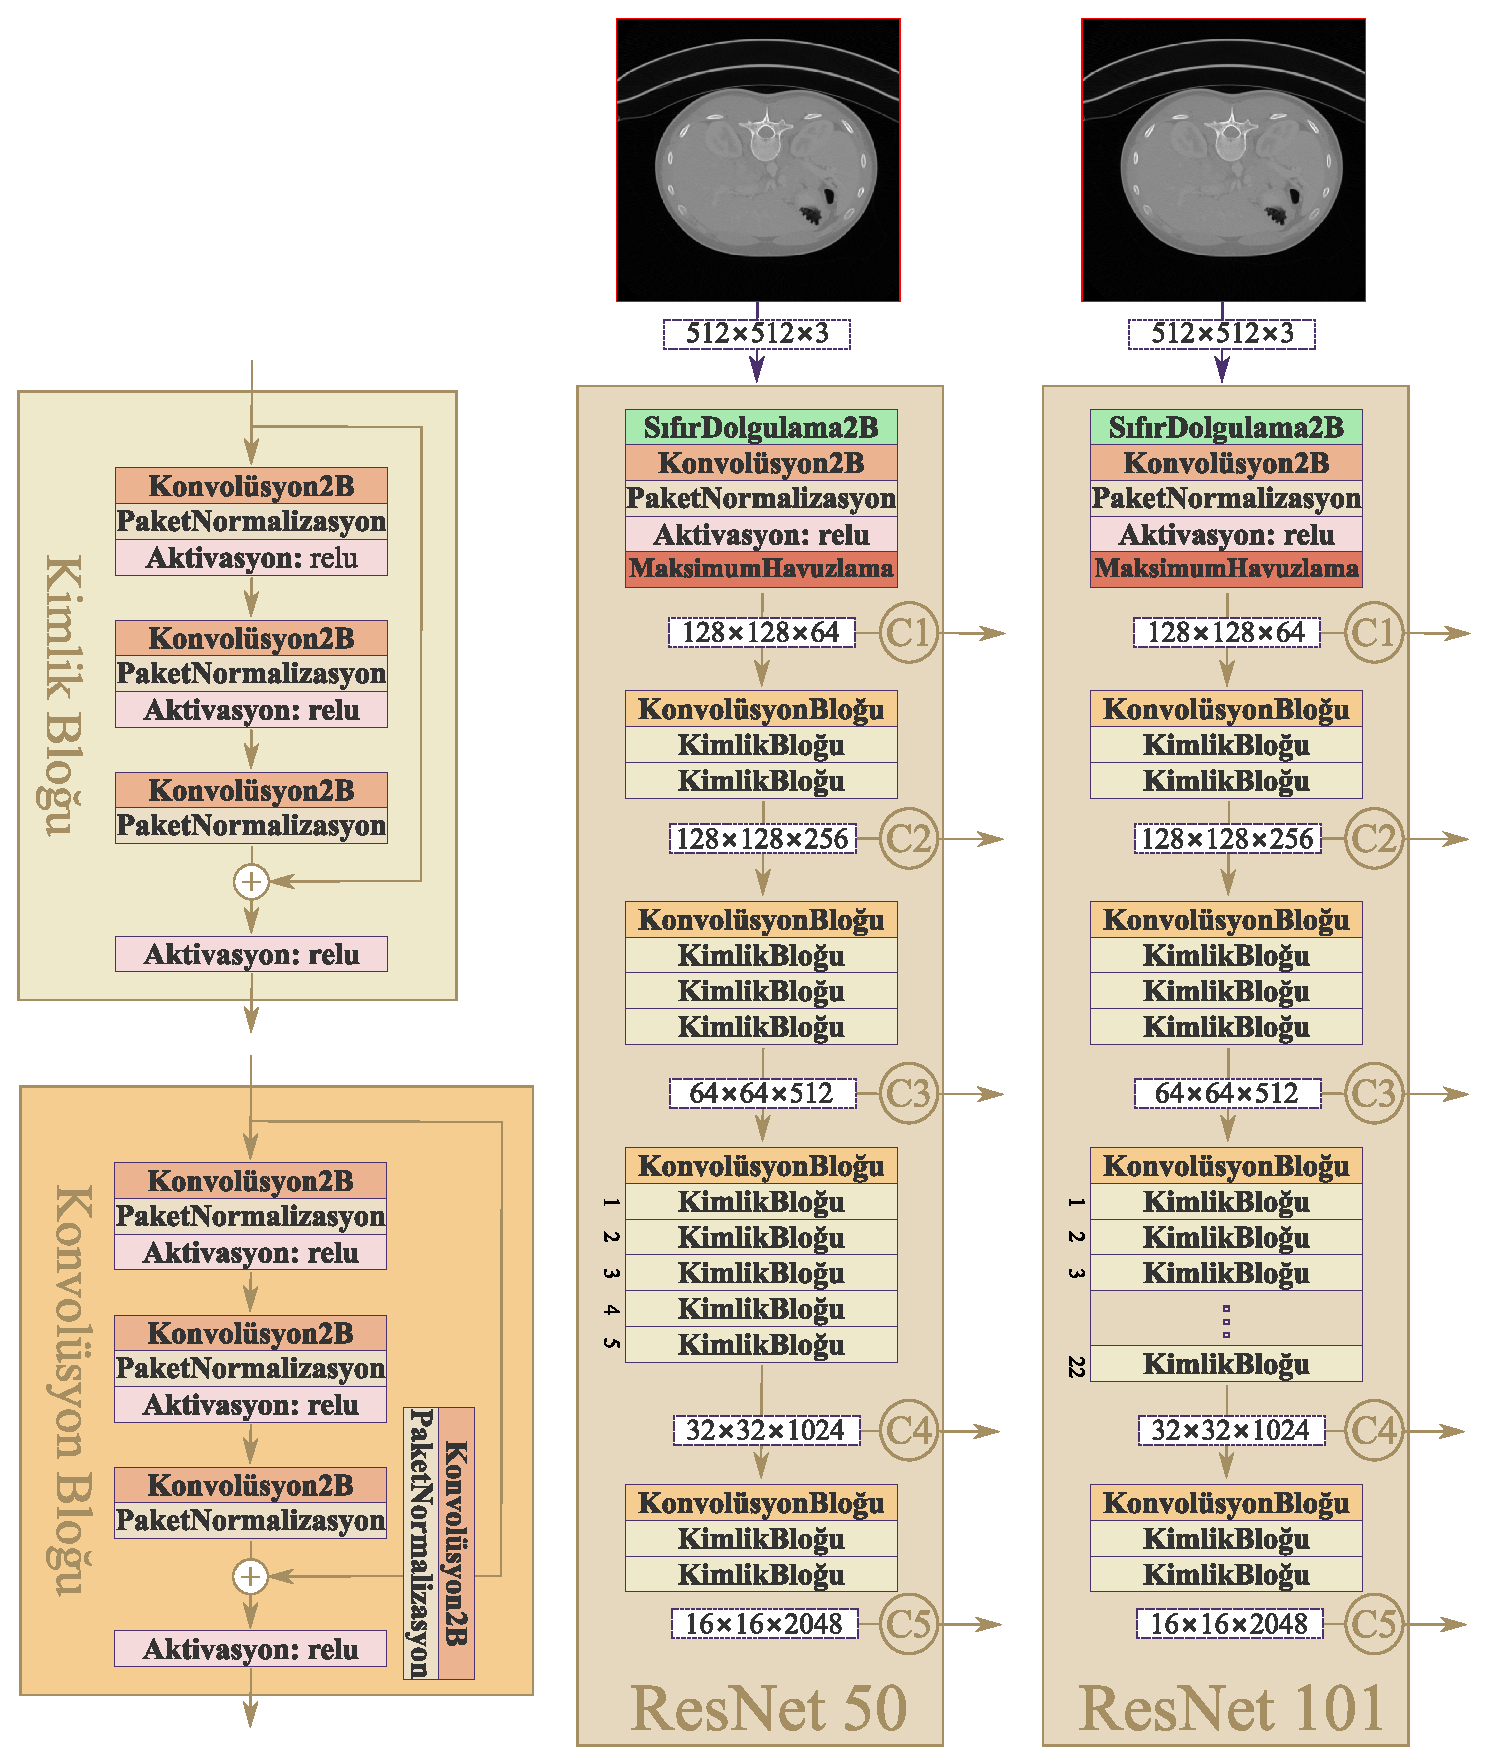
\includegraphics[scale=0.6]{Yapilan-Calismalar/Figures/head_network2.pdf}
		}
	\end{center}
\end{figure} 

Mask R-CNN modeli Şekil \ref{fig:maskrcnn}'da gösterildiği gibi Çekirdek Ağı, Özellik Piramit Ağı, Aday Bölge Çıkarım Ağı, Sınıflandırıcı Ağı ve Maske Üretim Ağı olmak üzere beş ana adımdan oluşmaktadır. Bu alt ağlardan biri olan Çekirdek Ağı kısmında pankreas organı için belirleyici özellik haritalarının üretilmesi gerçekleştirilmektedir. Diğer tüm alt ağlar ise bu özellik haritalarından elde edilen ön bilgi ile çalışmaktadır. Bu sebeple Mask R-CNN modelinin başarısını en fazla etkileyen alt adım olarak Çekirdek Ağı karşımıza çıkmaktadır. Literatürde CNN tabanlı farklı özellik çıkarıcılar kullanılarak Mask R-CNN modelinin performansındaki değişiklikleri incelemek mümkündür.


ResNet 50 ve ResNet 101 özellik çıkarıcıları kullanan Mask R-CNN modelinin şematik temsili Şekil \ref{fig:head_network2}'de verilmektedir. Şekil \ref{fig:head_network2}'de Çekirdek Ağı olarak ResNet-50 ve ResNet-101 CNN özellik çıkarıcıları kullanılması durumunda üretilen C1, C2, C3, C4 ve C5 çıkışları görülmektedir. Bir sonraki Özellik Piramit Ağı adımı üretilen C2, C3, C4 ve C5 çıkışları ile $1 \times 1$ konvolüsyon filtreleri kullanarak derinlikli konvolüsyonlama (depthwise convolution) işlemi gerçekleştirdiği için Çekirdek Ağı adımında üretilen çıkışların C2 ($128 \times 128 \times n$), C3 ($64 \times 64 \times n$), C4 ($32 \times 32 \times n$) ve C5 ($16 \times 16 \times n$) özellik haritalarının sayısını belirten $n$ değeri önemsizleşmektedir. C2, C3, C4 ve C5 çıkışlarından gelen özellik haritaları Özellik Piramit Ağı adımında kullanılarak P2 ($128 \times 128 \times 256$), P3 ($64 \times 64 \times 256$), P4 ($32 \times 32 \times 256$), P5 ($16 \times 16 \times 256$) ve P5 ($8\times 8 \times 256$) çıkışları üretilmektedir. Çekirdek Ağı'nın özellik çıkarıcı CNN modeli olarak $n$ ilgili katmandaki özellik haritası sayısını belirtmek üzere C2 ($128 \times 128 \times n$), C3 ($64 \times 64 \times n$), C4 ($32 \times 32 \times n$) ve C5 ($16 \times 16 \times n$) özellik haritalarını üretebilecek herhangi bir modelin kullanılması Mask R-CNN çalışmasını etkilememektedir. Bu sayede farklı çekirdek ağlar ile Mask R-CNN yönteminin kullanıldığı pankreas kaba bölgesinin tespiti gerçekleştirilebilmektedir.

Bu tez çalışmasında pankreas ve pankreas tümör segmentasyonu için 3 farklı model (3B Standart FCN Oto Kodlayıcı, 3B UNet ve 3B UNet++) performansları ayrı ayrı kullanılmaktadır.
Pankreas ve pankreas tümör segmentasyonu tek başına 2 sınıflı (diğer dokular, pankreas) pankreas segmentasyonundan farklı olarak 3 sınıflı (diğer dokular, pankreas, pankreas tümörü) bir segmentasyon problemidir.

3 sınıflı segmentasyon gerçekleştirilecek verilerde Pankreas İlgi Bölgesinin Belirlenmesi aşaması ile bölgenin küçültülmüş olmasına karşın hala sınıflar arasında dengeli bir voksel dağılımı mevcut değildir. Tümör dokuları bazı hastalarda pankreas ve diğer dokulara nazaran oldukça büyük yer tutmaktadır. Dengelenmemiş veriseti (imbalanced dataset) olarak adlandırılan bu probleme çözüm üretecek şekilde önerilen yöntemin ikinci aşaması olan hassas segmentasyon aşamasının güncellenmesi gerekmektedir. Dengelenmemiş veriseti probleminin önüne geçebilmek için CCE kayıp fonksiyonunun $\alpha$ ve $\gamma$ hiper parametreleri eklenerek özelleştirilmiş bir versiyonu olan FL kayıp fonksiyonu tercih edilmektedir. Ayrıca 3 modelde de (3B Standart FCN Oto Kodlayıcı, 3B UNet ve 3B UNet++) son katmanın aktivasyon fonksiyonu olarak softmax aktivasyon fonksiyonu kullanılmaktadır. CCE kayıp fonksiyonu türevi olan tüm kayıp fonksiyonlarında CCE kayıp fonksiyonunda olduğu gibi son katman aktivasyon fonksiyonu olarak softmax aktivasyon fonksiyonu tercih edilmektedir. Böylece girişten uygulanan herbir hastaya ait volümetrik BT verisinden 3 farklı (diğer dokular, pankreas, pankreas tümörü) sınıfı temsilen volümetrik maske verileri üretilmektedir.

\subsection{Belirlenen İlgi Bölgesinde Pankreas ve Pankreas Tümör Segmentasyonu Gerçekleştirmek Amacıyla Denenen Farklı Derin Ağ Modelleri}

BU tez çalışmasında volumetrik BT görüntülerinde pankreas ve pankreas tümör segmentasyonu gerçekleştirmek için 3 farklı derin ağ segmentasyon modeli kullanılmıştır. BU modeller sırasıyla 3B FCN Oto Kodlayıcı modeli, 3B UNet modeli ve 3B UNet++ modelidir. 

\subsubsection{3B FCN Oto Kodlayıcı Modeli ile Pankreas ve Pankreas Tümör Segmentasyonu}
Oto kodlayıcılar çeşitli amaçlar için kullanılabilmekle birlikte segmentasyon problemlerinde de sıklıkla tercih edilmektedir. Bu tez çalışmasında kullanılan 3B oto kodlayıcı modeli standart oto kodlayıcılara uygun şekilde ele alınmakta ve 3 sınıflı (diğer dokular, pankreas, pankreas tümörü) probleme uygun şekilde yeniden dizayn edilmektedir. Pankreas ve Pankreas Tümörü Segmentasyonunda kullanılan 3B FCN Oto Kodlayıcı'nın şematik temsili Şekil \ref{fig:3dotokod}'da verilmektedir. Standart bir oto kodlayıcı temelde kodlama ve kod çözme aşamasından oluşmaktadır. Girişten uygulanan veri ardışık konvolüsyon katmanları ile kodlanmakta yani manuel olarak işaretlenmiş volümetrik maske verileri kullanılarak volümetrik BT verilerinin özellik haritaları çıkarılmaktadır. Pankreas İlgi Bölgesinin Belirlenmesi aşaması ile $192 \times 256 \times 256$ ölçeklerine indirgenen volümetrik giriş verisi ardışık konvolüsyon işlemine tabi tutularak kodlama aşamasında $3 \times 4 \times 4$ ölçeklerine kadar indirgenerek kodlama işlemi gerçekleştirilmektedir. Daha sonra çıkarılan bu özellik haritalarına ardışık ters konvolüsyon katmanları ile kod çözme işlemi gerçekleştirilmekte yani öğrenilen özellik haritalarından tahmin maskesi volümetrik verileri inşa edilmektedir. Bu aşamada $3 \times 4 \times 4$ ölçeklerine indirgenmiş özellik haritaları ardışık ters konvolüsyon işlemlerinin ardından $96 \times 128 \times 128$ ölçeklerine çıkarılmaktadır. Daha sonra tekrar bir ters konvolüsyon işlemi softmax aktivasyon fonksiyonu ile kullanılarak 3 adet $192 \times 256 \times 256$ ölçeklerinde tahmin maskeleri üretilmektedir.  

\captionsetup[figure]{margin={0.4cm,-1.5cm}}
\begin{figure}[h!]
	\begin{center}
		\vspace{0.4cm}
		\captionbox{Pankreas ve Pankreas Tümörü Segmentasyonunda kullanılan 3B FCN Oto Kodlayıcı'nın şematik temsili.\label{fig:3dotokod}}
		{
			\vspace{0.4cm}
			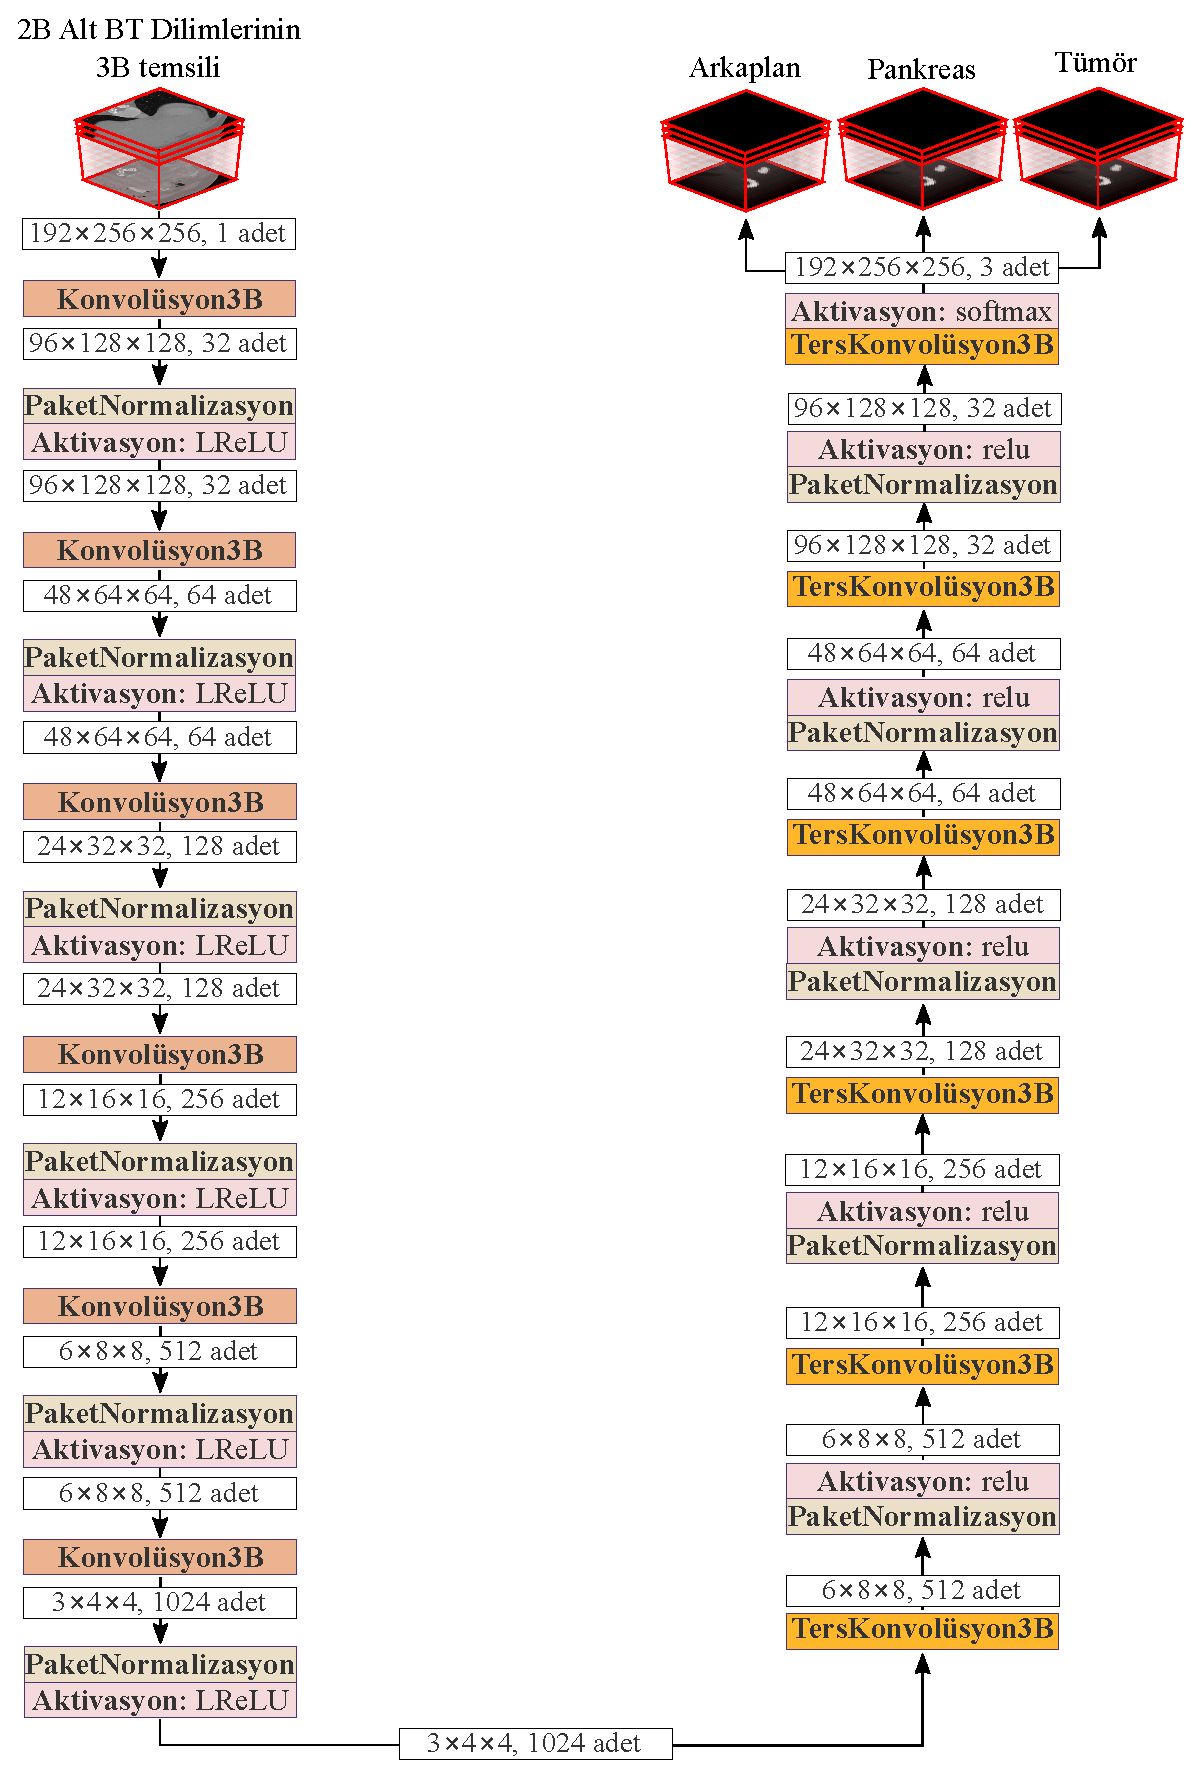
\includegraphics[scale=0.6]{Yapilan-Calismalar/Figures/3dfcn.pdf}
		}
	\end{center}
\end{figure} 

Üretilen tahmin maskeleri sırası ile diğer dokular, pankreas ve pankreas tümörünü temsil eden volümetrik verilerdir. Aslında üretilen bu 3 farklı volümetrik maske verisinde her bir voksel için softmax aktivasyon fonksiyonu ile 3 sınıfı temsilen 3 farklı çıkış üretilmektedir. Yani voksel ölçeğinde bir sınıflandırma işlemi gerçekleştirilerek segmentasyon yapılmaktadır.

Bu tez çalışmasında öncelikle 3B Standart FCN Oto Kodlayıcı modelini tercih etmekteki amaç 3B U-Net yaklaşımındaki atlama bağlantılarının (skip conections) segmentasyona etkilerinin incelenmesidir. Standart FCN Oto Kodlayıcı modellerinin atlama bağlantıları eklenerek özelleştirilmiş versiyonu olan U-Net yaklaşımı ardışık konvolüsyon katmanlarında derinlik arttıkca kaybedilen özelliklerin geri kazanımını hedeflemektedir.

\subsubsection{3B U-Net Modeli ile Pankreas ve Pankreas Tümör Segmentasyonu}
Oto kodlayıcıların atlama bağlantıları (skip connections) eklenerek güçlendirilmiş versiyonu olan U-Net yaklaşımı ardışık konvolüsyon katmanlarında yaşanan bilgi kaybının önüne geçmeyi amaçlamaktadır. Pankreas ve Pankreas Tümörü Segmentasyonunda kullanılan 3B U-Net modelinin şematik temsili Şekil \ref{fig:3dunet2}'da verilmektedir. Oto kodlayıcılarda olduğu gibi 3B U-Net modeli de girişinden girdi olarak aldığı volümetrik verilerde ardışık konvolüsyon işlemi gerçekleştirerek kodlama işlemi gerçekleştirmekte ve daha sonra giriş verisinden elde edilen özellik haritaları üzerinde ters konvolüsyon katmanları ile ters yönde kod çözme işlemi gerçekleştirmektedir.

\captionsetup[figure]{margin={0.4cm,-1.5cm}}
\begin{figure}[h!]
	\begin{center}
		\vspace{0.4cm}
		\captionbox{Pankreas ve Pankreas Tümörü Segmentasyonunda kullanılan 3B U-Net modelinin şematik temsili.\label{fig:3dunet2}}
		{
			\vspace{0.4cm}
			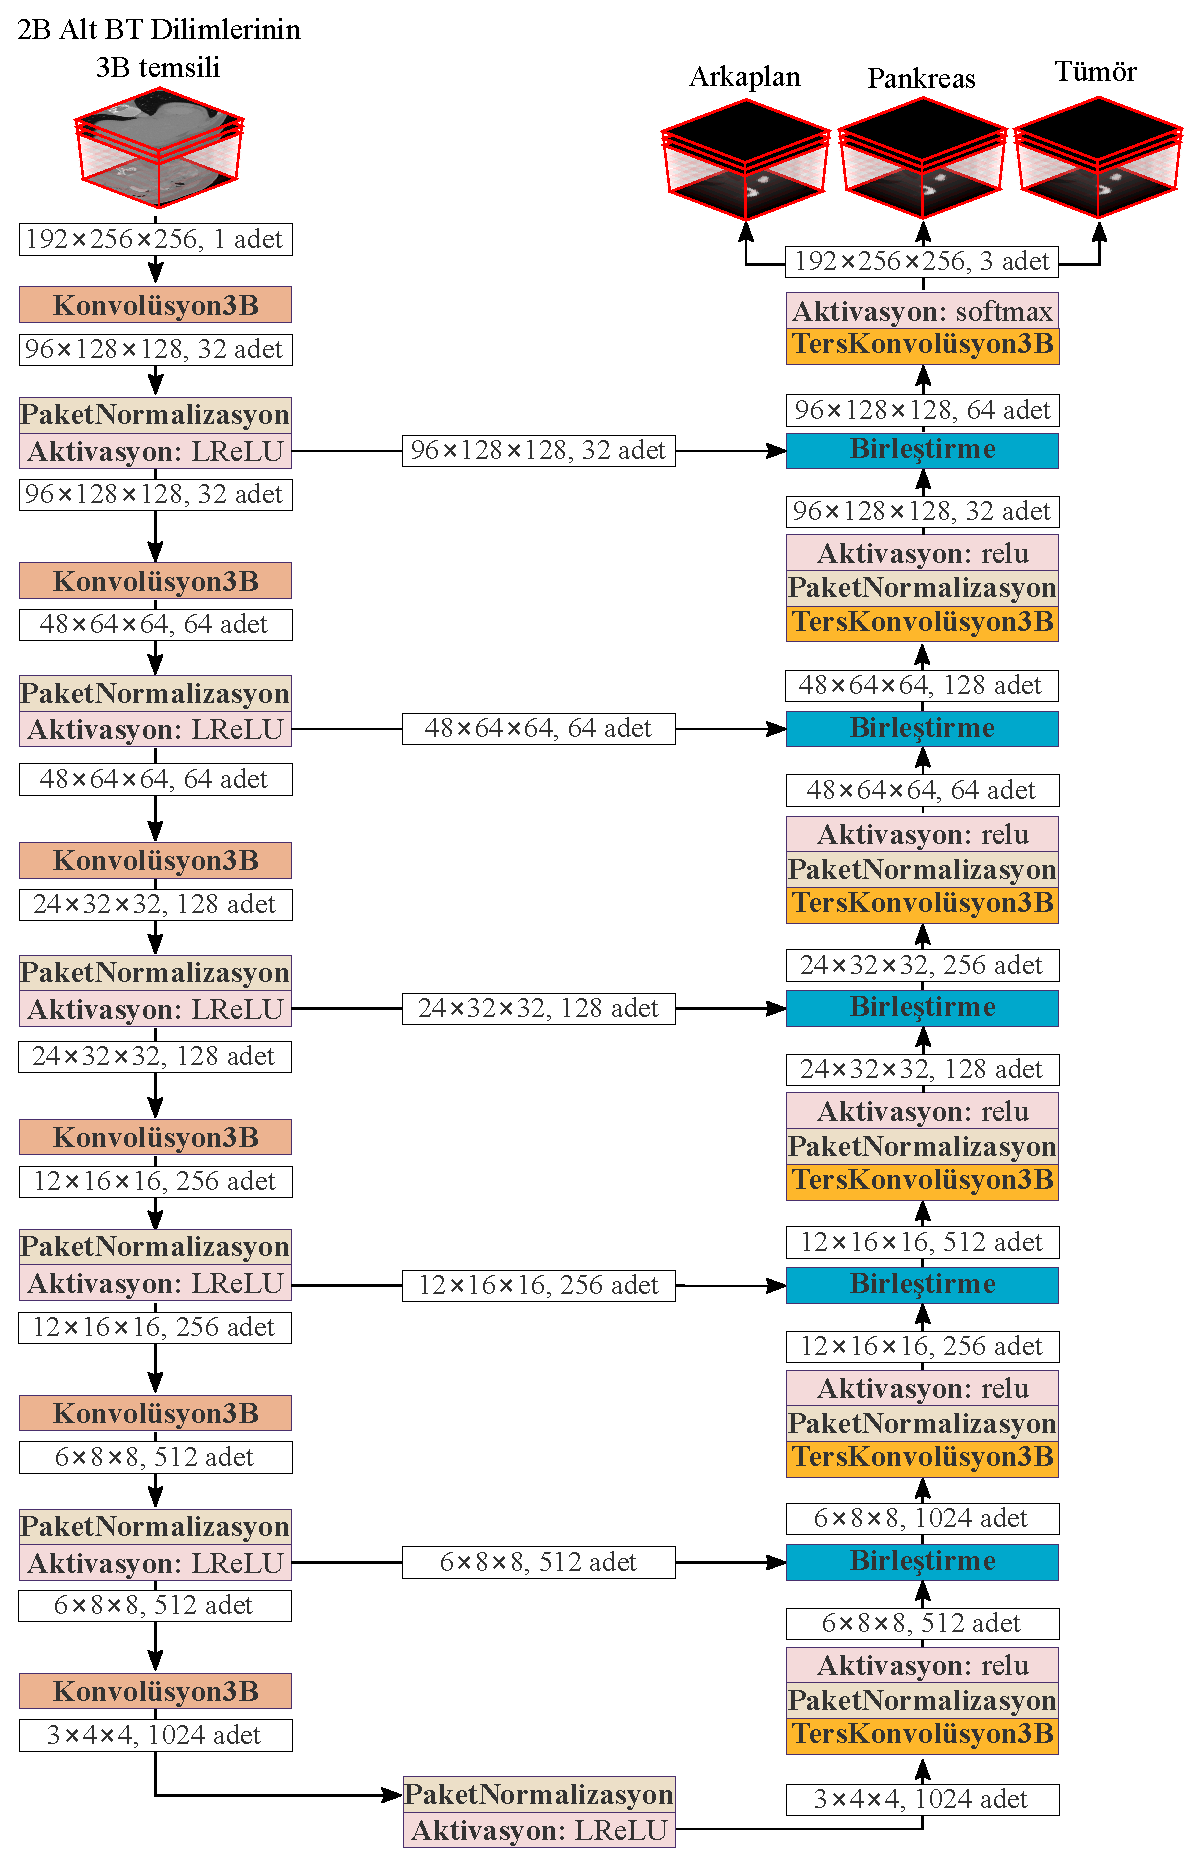
\includegraphics[scale=0.6]{Yapilan-Calismalar/Figures/3dunet2.pdf}
		}
	\end{center}
\end{figure} 

Bu tez çalışmasında pankreas segmentasyonu için önerilen yöntemin segmentasyon aşamasında kullanılan 3B U-Net modelinden farklı olarak pankreas ve pankreas kanser dokularının segmentasyonu için geliştirilen 3B U-Net modelinde üç sınıflı(diğer dokular, pankreas, pankreas tümörü) segmentasyon gerçekleştirebilen bir model üretilmektedir. Böylece standart oto kodlayıcılardan farklı olarak eklenen atlama bağlantılarının segmentasyona etkileri incelenmektedir. Şekil \ref{fig:3dunet2}'da detayları gösterilen 3D U-Net modelinde girişinden Pankreas İlgi Bölgesinin Belirlenmesi aşaması ile küçültülmüş $192 \times 256 \times 256$ ölçeklerinde volümetrik BT alt görüntüleri uygulanmaktadır. Bu veriler ardışık konvolüsyon katmanları ile küçültülerek (kodlama) sırasıyla $96 \times 128 \times 128$, $48 \times 64 \times 64$, $24 \times 32 \times 32$, $12 \times 16 \times 16$, $6 \times 8 \times 8$ ve $3 \times 4 \times 4$ ölçeklerine indirgenmektedir. Bu özellik haritaları ters konvolüsyon işlemleri ile ters yönde ölçek artımına tabi tutulmaktadır. Ters konvolüsyon sonucu ölçeği büyütülen özellik haritaları kodlama aşamasından gelen eşit ölçekli özellik haritaları ile birleştirilmektedir. Ters yönde (kod çözme) $96 \times 128 \times 128$ ölçeğine gelindiğinde son bir ters konvolüsyon işlemi softmax aktivasyon fonksiyonu ile kullanılarak 3 adet $192 \times 256 \times 256$ ölçeklerinde tahmin maskeleri üretilmektedir. Bu tahmin maskeleri sırası ile diğer dokular, pankreas ve pankreas tümörünü temsil eden volümetrik verilerdir. Aslında üretilen bu 3 farklı volümetrik maske verisinde herbir voksel için softmax aktivasyon fonksiyonu ile 3 sınıfı temsilen 3 farklı çıkış üretilmektedir. Yani voksel ölçeğinde bir sınıflandırma işlemi gerçekleştirilerek segmentasyon yapılmaktadır.  


\subsubsection{3B U-Net++ Modeli ile Pankreas ve Pankreas Tümör Segmentasyonu}
3B U-Net modelinde atlama bağlantılarının önemi irdelenirken 3B U-Net++ modelinde daha karmaşık atlama bağlantıları ile bir anlamda iç içe U-Net modellerinin performansa etkileri irdelenmektedir. U-Net++ yaklaşımı atlama bağlantılarının çok daha kompleks kullanıldığı bir model olarak karşımıza çıkmaktadır. Pankreas ve Pankreas Tümörü Segmentasyonunda kullanılan 3B U-Net++  modelinin şematik temsili Şekil \ref{fig:3dunet++}'de verilmektedir. 

\captionsetup[figure]{margin={0.4cm, 0.2cm}}
\begin{figure}[h!]
	\begin{center}
		\vspace{0.4cm}
		\captionbox{Pankreas ve Pankreas Tümörü Segmentasyonunda kullanılan 3B UNet++ modelinin şematik temsili.\label{fig:3dunet++}}
		{
			\vspace{0.4cm}
			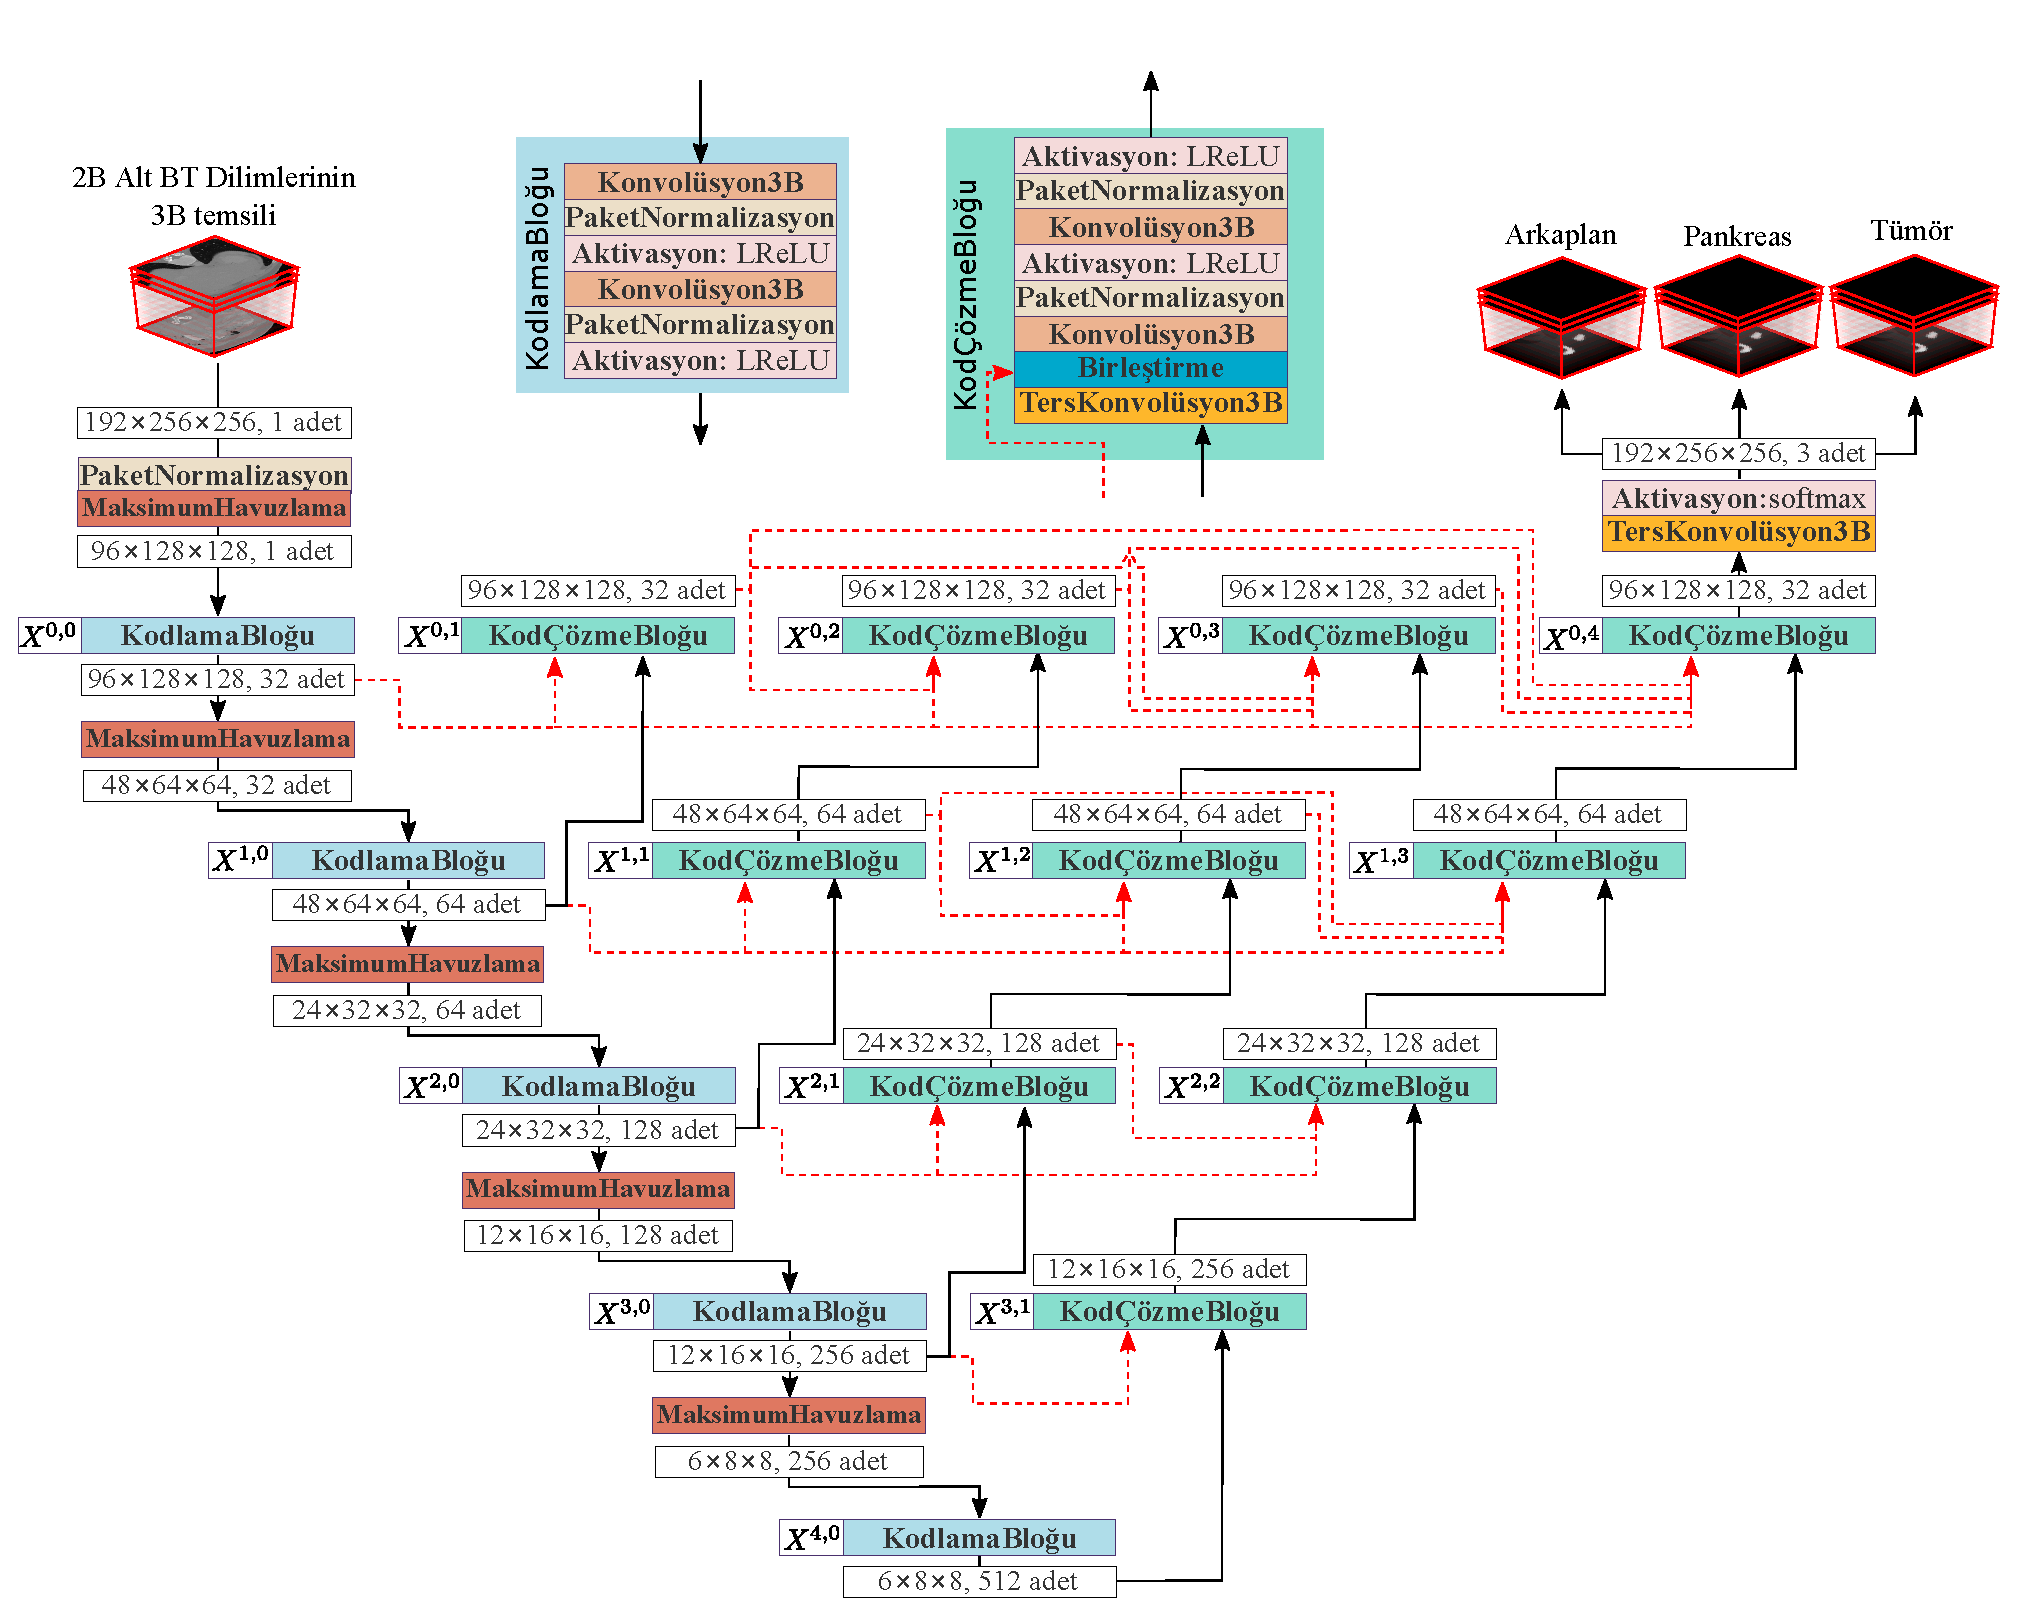
\includegraphics[scale=0.45]{Yapilan-Calismalar/Figures/3dunet++.pdf}
		}
	\end{center}
\end{figure} 

3B U-Net++ yönteminde atlama bağlantılarının çokluğundan kaynaklı hesaplama maliyetini düşürmek adına kodlama aşamasında ölçek azaltma işleminde konvolüsyon katmanları yerine maksimum havuzlama katmanları ile gerçekleştirilmektedir. Konvolüsyon katmanlarında özellik haritalarının ölçekleri dolgulama ile korunmaktadır.

3B U-Net++ modeli temelde iç içe U-Net modellerinden oluşmaktadır. U-Net++ modelinin girişinden Pankreas İlgi Bölgesinin Belirlenmesi aşaması ile küçültülmüş $192 \times 256 \times 256$ ölçeklerinde volümetrik BT alt görüntüleri uygulanmaktadır. Sırası ile $X^{0,0}$,$X^{1,0}$ ve $X^{0,1}$ blokları en küçük U-Net alt ağını temsil etmektedir. İkinci seviyeden U-Net modeli sırasıyla $X^{0,0}$, $X^{1,0}$, $X^{2,0}$, $X^{1,1}$ ve $X^{2,0}$ blokları ile temsil edilmektedir. Üçüncü seviyeden U-Net modeli sırasıyla $X^{0,0}$, $X^{1,0}$, $X^{2,0}$, $X^{3,0}$, $X^{2,1}$, $X^{1,2}$ ve $X^{0,3}$ blokları ile temsil edilmektedir. Son olarak dördüncü U-Net modeli sırasıyla $X^{0,0}$, $X^{1,0}$, $X^{2,0}$, $X^{3,0}$, $X^{4,0}$, $X^{3,1}$, $X^{2,2}$, $X^{1,3}$ ve $X^{0,4}$ blokları ile temsil edilmektedir. Görüldüğü gibi U-Net++ yöntemi iç içe U-Net modellerinden oluşmaktadır. Modelin $X^{4,0}$ blok çıkışı $96 \times 128 \times 128$ ölçeğinde veri üretmekte ve bu veri son bir ters konvolüsyon işlemine tabi tutulmaktadır. Konvolüsyon işleminin çıkışı softmax aktivasyon fonksiyonuna tabi tutularak 3 adet $192 \times 256 \times 256$ ölçeklerinde tahmin maskeleri üretilmektedir. Bu tahmin maskeleri sırası ile diğer dokular, pankreas ve pankreas tümörünü temsil eden volümetrik verilerdir. Aslında üretilen bu 3 farklı volümetrik maske verisinde her bir voksel için softmax aktivasyon fonksiyonu ile 3 sınıfı temsilen 3 farklı çıkış üretilmektedir. Yani voksel ölçeğinde bir sınıflandırma işlemi gerçekleştirilerek segmentasyon yapılmaktadır.